% Template author: Johannes Demel
% Document class provides standardized title page + needed extras.
\documentclass{cel-thesis/cel-thesis}
\thesisTitle{Evaluation of Machine Learning and Deep Neural Networks for Cognitive Radio Interweave Systems}
\thesisType{Master's Thesis}
\thesisAuthor{Nicolas Cuervo-Benavides}
\thesisAdvisor{Dr.-Ing. Holger Jäkel}
\thesisHeadOfInstitute{}
%\thesisHeadOfInstitute{Dr.-Ing. Holger Jäkel}
\thesisSupervisor{M.Sc. Felix Wunsch}
\thesisStartDate{17th May 2017}
\thesisEndDate{6th December 2017}
\thesisSignatureDate{06.12.2017}
\thesisLanguage{english} % english or ngerman
\thesisCC{FALSE}
\thesisPythonWatermark{FALSE}


%%% LANGUAGE SETTINGS %%%%%%%%%%%%%%%%%%%%%%%%%%%%%%%%%%%%%%%%%%%%%%%%%%%%%
% additional Hyphenation rules
\hyphenation{non-para-metric repro-gra-mmable}
% Settings for bibliography
\usepackage{babelbib}
\setlanguage % set correct language as selected above

%%% PACKAGES %%%%%%%%%%%%%%%%%%%%%%%%%%%%%%%%%%%%%%%%%%%%%%%%%%%%%%%%%%%%%%%%%
% Add all the packages you feel like you need them.
% You'll need it.
% automatically expand/abbreviate terms.
\usepackage{caption}
\usepackage{subcaption}
\usepackage{todonotes} % great for draft annotations

% Added additionally to the template
\definecolor{kit-green100}{rgb}{0,.59,.51}
\definecolor{kit-green70}{rgb}{.3,.71,.65}
\definecolor{kit-green50}{rgb}{.50,.79,.75}
\definecolor{kit-green30}{rgb}{.69,.87,.85}
\definecolor{kit-green15}{rgb}{.85,.93,.93}
\usepackage{url}
\def\UrlBreaks{\do\/\do-\do\_}
\usepackage{hyperref}
\usepackage{xcolor}
\usepackage{listings}
\usepackage{amsmath}
\colorlet{cyan}[rgb]{cyan}
\usepackage{standalone} % To add tikz figure as standalone elements
\usepackage{tikz}  % To add tikz figures
\usepackage{array} % To use alignment such as m{} or b{} in tables
\usetikzlibrary{datavisualization}
\usetikzlibrary{positioning}
\usetikzlibrary{arrows,calc,fit}
\usetikzlibrary{shadows}
\usetikzlibrary{mindmap}
\tikzset{line/.style={draw, thick, -latex'}}

\setcounter{tocdepth}{4}
\setcounter{secnumdepth}{4}

%%% DEFINITIONS %%%%%%%%%%%%%%%%%%%%%%%%%%%%%%%%%%%%%%%%%%%%%%%%%%%%%%%%%%%%%%%%%

%% pretty C++ print.
\def\CC{{C\nolinebreak[4]\hspace{-.05em}\raisebox{.4ex}{\tiny\textbf{++}}}}

\begin{document}
\makeatletter
    \setlength\@fptop{0\p@}
\makeatother
\pagenumbering{roman}  % all the preliminaries should be counted roman style
\maketitle
%% preliminaries
  \chapter*{Abstract}

This thesis evaluates different machine learning techniques for effective spectrum awareness on \ac{CR} interweave systems. In the last decades, access to the electromagnetic spectrum has been granted to the highest bidder on \emph{spectrum auctions}. The auction winner is thereafter entitled to use a definite portion of the spectrum in a way which fits the best to the technology or service that he wants to provide. But, with increasing demand for this natural resource, it is imperative to find techniques that allow a more effective use of the spectrum, such as spectrum sharing.\\

Spectrum sharing has been an ongoing topic of research in the last few years for the purpose of being part of the 5G communications systems, as well as for generally mitigating spectrum scarcity. The \ac{CEL} has actively worked on this issue with the use of \ac{SDR} and \ac{CR} devices. \ac{CR} devices have, conceptually, a \emph{learning stage} where they observe signals from the outer world in order to learn how to react accordingly, which consequently serves as a catalyst for the introduction of \ac{ML} to accomplish this purpose. Recently, \ac{CEL} has very successfully taken part in the \ac{DySpan} spectrum challenge competitions which deal specifically with this matter. In these competitions, a communication system with higher priority, also known as a \ac{PU}, is set to make use of a certain central frequency and \ac{BW} (divided into four channels) sending packets in a bursty fashion, randomizing the way it accesses the spectrum over ten different scenarios that vary its channel ocupation, frequency hopping pattern, packet length and inter-packet delay. The objective of these competitions is to implement a communication system with lesser priority, also known as a \ac{SU}, that identifies effectively the scenario that the \ac{PU} is using, and takes advantage of this information to access the spectrum in a way that interferes the least with the ongoing communication. This thesis uses the DySpan Spectrum Challenge 2017 setup as testbed and focuses on evaluating techniques used to identify the way the \ac{PU} is accessing the spectrum by the means of \ac{ML} and \ac{DL}.\\

Within the implementation of the challenge's testbed the specific scenario that the \ac{PU} uses for its transmission can be controlled, and this ability is used to record labeled samples over the specified bandwidth during a certain amount of time in order to generate a composite dataset, from which the scenarios that it uses are learned thenceforth using supervised learning. Additionally, the transmission power of the \ac{PU} is also varied in order to generate samples with different \ac{SNR}, to ensure that the \ac{ML} models learn how to classify under a diversity of signal power conditions. The learning methods are separated into two categories, based on the type of preprocessing that input data undergoes:

\paragraph*{Feature-based learning:} specific information is extracted from the recorded data as so-called \emph{features}, and then is used as an input into \ac{ML} algorithms. Then a benchmark between the K-nearest neighbors, decision trees, and \ac{SVM} is presented demostrating how well these algorithms are able to classify the correct scenario based on the extracted features. This method relies on a energy detection scheme to generate the features, which presents a limitation when the \ac{PU} is transmitting with low SNR.
\paragraph*{Spectrogram-based learning:} data preprocessing here consist of generating spectrograms that are fed into convolutional neural networks for them to be classified using image recognition techniques. Different optimizers, such as the stochastic gradient descent, adamax, and adadelta, are used to achieve an understanding of their convergence speed as well as their accuracy. This method is independent of the \ac{PU} SNR, as the spectrograms are generated directly from the input data regardless of its spectral content.\\

The performance of these methods is analyzed with respect to their accuracy on classification over the test dataset, along with the time they take to classify a data sample. These parameters serve as figures of merit to determine how viable it is to use these algorithms in real-time applications. Lastly, a demonstration of the performance of the regarded classification models is presented using GNU Radio, where the \ac{PU} scenarios are classified in real-time. This work shows that with a relatively little amount of data confident spectrum awareness can be achieved using learning techniques, without the need of pinning down a specific analytical description of the way the spectrum is being utilized by other actors in a communication system.\\

This thesis culminates in a conclusion on the feasibility of using the analyzed \ac{ML} algorithms in real-time scenarios. Based on the results achieved, it can be confidently affirmed that decision trees provide the best trade off between accuracy and prediction time for this specific use case for feature-based classification. On the counterpart, \ac{SVM} do not provide satisfactory results, having a about 10\% less accuracy than the other two analyzed models while taking about 2500 times longer to provide a prediction than decision tree classifiers, and about 50 times longer than K-nearest neighbors classifier prediction, making them unsuitable for this application. Furthermore, it is found that image classification using a convolutional neural network with the adadelta optimizer provides a reliable classifier with as little as 300 iterations of training, which makes the spectrogram-based learning appealing over the feature-based learning as it does not depend on the \ac{PU} signal power to provide a prediction.
		% a MUST, few pages abstract

%% main document
\cleardoublepage
\pagenumbering{arabic} % now old school arabic enumerated pages.
  \tableofcontents 		% a MUST
  \cleardoublepage		% make sure multipage TOCs are numbered correctly.
  \acresetall
\chapter{Introduction}\label{ch:intro}

Back in 1999, Joseph Mitola III coined the term \ac{CR}\cite{Mitola1999} as a way to enhance the \ac{SDR} capabilities by the means of a dynamic model that, based on human intervention, improved the flexibility of devices by making them fully configurable and capable of adapting to the communication system's needs, suitable to react to the changes in the environment. A formal definition for the \ac{CR} concept provided at \cite{Haykin2005} encloses the term nicely by describing it as a wireless system that is \emph{intelligent and aware of its surroundings}, whilst being able to learn, adapt and react to changes in the ambience, by modifying its operation parameters such as the transmission power, the modulation scheme, and its carrier frequency in real-time. Analogously, Jondral \cite{Jondral2005} adopts the short definition for \ac{CR} as "an \ac{SDR} that additionally senses its environment, tracks changes, and possibly reacts upon its findings", becoming an autonomous unit with the potential of using the spectrum efficiently.\\

\ac{CR} systems are intended to be immersed in a network, where it interacts with other systems that could be cognitive or non-cognitive radios. According to \cite{Goldsmith}, \ac{CR} is grouped under three paradigms: underlay, overlay and interweave. The \emph{Underlay Paradigm} allows the \ac{CR} system to operate under acceptable levels of interference, determined by an interference threshold. Here, the \ac{CR} is commonly called a \ac{SU}, providing priority to the other systems in the network which it should not significantly interfere, known also as \ac{PU}. In the \emph{Overlay Paradigm}, the cognitive transmitter knows information about the other transmitters in the network, such as their codebooks and modulation schemes. In addition, this model assumes that message that is being transmitted is known by the \ac{CR} when transmission by a non-cognitive system is initiated. This provides the cognitive system with multiple choices on how to use this information: for instance, it can be used to mitigate or completely cancel a possible interference happening in the network during transmission. Additionally, the cognitive system could also retransmit this message to other non-cognitive systems in the network, acting as a relay and, effectively, assist increasing the \ac{SNR} of the non-cognitive system to a level equivalent to the possible decrease due to the interference caused by \ac{CR} transmissions. The \emph{Interweave Paradigm}, or opportunistic communication, identifies temporary space-time-frequency gaps where it can intelligently allocate its transmission, increasing the available resource utilization and minimizing the interference with other active users. Hybrid schemes are also actively being developed \cite{Wu2007} \cite{Kaushik2015} \cite{Wunsch2017a}, where characteristics from different paradigms are combined in order to achieve an effective use of the available communication's resources.\\

The main characteristic required to apply any of the aforementioned paradigms is awareness, being it in regards to location, spectrum, time, etc. Awareness is achieved by the means of \emph{the cognition cycle} \cite{Mitola1999}, shown in Fig.~\ref{fig:cognition_cycle}, which enfolds the way the \ac{CR} parses the stimuli from the outside world in order to plan accordingly the proper reactions. This cognition cycle revolves around the following concepts:

\begin{figure}[htb]
    \centering
      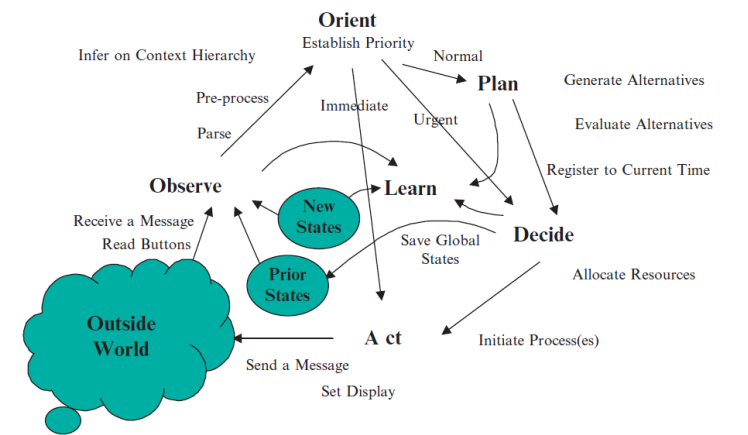
\includegraphics[width=0.8\textwidth]{figures/cognition_cycle.png}
      \caption{The cognition Cycle\cite{Mitola1999}}
      \label{fig:cognition_cycle}
\end{figure}

\begin{itemize}
    \item Observation: the \ac{CR} receives any signals from the external world, which can contain any type of information that the system can use in its favor and the favor of a better use of its resources.
    \item Orientation: The \ac{CR} determines the priority from the received signal as well as the type of reaction based on it.
    \item Planning: results from a normal-level priority, where a plan is generated and the sequence of actions to be taken are established.
    \item Decision: selects among the plan candidates the best proposal and allocates the necessary resources for its carrying-out.
    \item Acting: initiates action based on the previous taken decisions.
    \item Learning: is an integration of observations and decisions, based on past and current states that are compared with expectations. When an expectation is met, the system achieves effectiveness. When not, observations are recorded and kept for further learning.
\end{itemize}

These aspects of \ac{CR} come in handy when trying to solve one of the current major issues of communication systems: spectrum scarcity. The access to radio spectrum is highly regulated by government agencies such as the \ac{Ofcom}, the \ac{FCC} and the \ac{ITU}, and its access has been historically granted to the highest bidder on so-called \emph{spectrum auctions} \cite{Jondral2005} \cite{Staple2004}. Therefore, the seek of new technologies that allow a more efficient access to the spectrum is paramount. In an effort to find effective solutions for this increasing issue, the \ac{IEEE} created a Standards Committee back in 2005 which, in association with the \ac{ComSoc} and the \ac{EMC} dealt with the generation of standards for dynamic spectrum management. This committee was dissolved between 2007 and 2010 and, after organizational restructuring, the functions of standardization and spectrum management was handed to the \ac{SCC} - \ac{DySpan} \cite{IEEEDySPAN2015}. As part of these efforts to motivate state-of-art research in these regards, \ac{DySpan} has organized since 2007 the \emph{IEEE International Symposium on Dynamic Spectrum Access Networks} \cite{Comsoc}. Additionally, \ac{DySpan} has emboldened the healthy competition since 2015 by introducing the \emph{Spectrum Challenge}, which consists on inviting teams from all over the world to solve a problem related with dynamic access to the spectrum and 5G implementations. The participating teams are given a set of requirements and limitations but are encouraged to push these limits with creativity and innovation. The \ac{KIT}, represented by the \ac{CEL}, has taken part in these competitions achieving outstanding results, being awarded the \emph{Subjective Winner} award on 2015 \cite{Kaushik2015} and the \emph{Best Overall Solution} on 2017 \cite{Wunsch2017a}. This thesis utilizes the setup used in the 2017 spectrum challenge as a base testbed. Fig.~\ref{fig:dyspan_setup} shows the main characteristics of this setup.

\begin{figure}[htb]
    \centering
      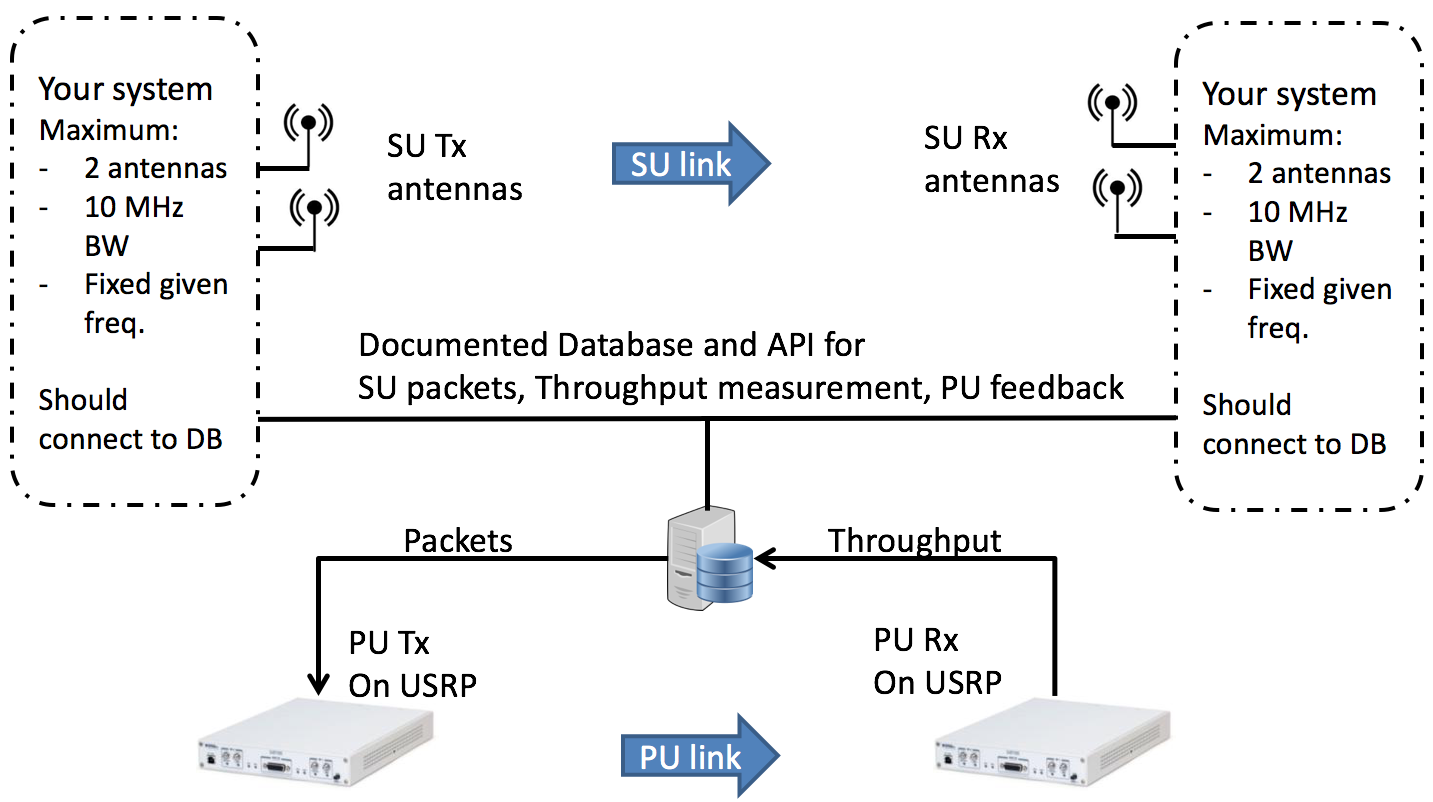
\includegraphics[width=0.8\textwidth]{figures/dyspan_set.png}
      \caption{The DySpan Spectrum Challenge Setup \cite{Dyspanchalle}}
      \label{fig:dyspan_setup}
\end{figure}

By using this configuration and keeping the hardware and overall physical considerations (such as \ac{BW}, number of antennas and central frequency),
the idea of the challenge was to achieve the maximum throughput between the proposed \ac{SU} systems, while interfering as little as possible with the existing \ac{PU}. The competition consisted of two phases: during phase one the situational awareness of the proposed \ac{CR} system is put under test, as it is needed to correctly identify the set of \ac{PU} transmission parameters:

\begin{itemize}
    \item Bandwidth and Carrier Frequency: Along the 10MHz of maximum \ac{BW} divided into four subchannels of 2.5MHz each, it needs to be detected if the \ac{PU} is using one, two or four channels for its transmission. Effectively, it is needed to determine which frequencies are being used (identify the frequency hopping pattern) and when are they being used.
    \item Packet description: The \ac{PU} transmitter sends packets in a bursty fashion to the corresponding receiver using packets of 64B payload.
    \item Inter-arrival time between packets: the time between a packet transmission might vary from a situation to another. These times could be deterministic for some scenarios, as well as stochastic for others following a Poisson distribution. Correctly identifying the interpacket time of the current situation allows for effective opportunistic access to the spectrum.
\end{itemize}

With these characteristics a set of 10 different scenarios is built, whose parameters are depicted in Table~\ref{table:scenarios}.

\begin{table}[h!]
    \centering
    \caption{Scenario description}
    \label{table:scenarios}
    \begin{tabular}{| >{\centering}m{5em}| m{12cm} |}
        \hline
        \textbf{Scenario} & \multicolumn{1}{|c|}{\textbf{Description}} \\
        \hline\hline
        0 & Single random channel, deterministic interpacket delay of 5ms \\\hline
        1 & Single random channel, deterministic interpacket delay of 10ms\\\hline
        2 & Two random channel hopping, deterministic interpacket delay of 5 ms\\\hline
        3 & Four random channel hopping, deterministic interpacket delay of 10 ms\\\hline
        4 & Two random channel hopping, deterministic interpacket delay of 5ms\\\hline
        5 & Four synchronous channels, deterministic interpacket delay of 5ms\\\hline
        6 & Four synchronous channels back-to-back, deterministic interpacket delay of 2ms\\\hline
        7 & Four asynchronous random channels, Poisson distributed interpacket delay with mean of 20ms\\\hline
        8 & Four asynchronous random channels, Poisson distributed interpacket delay with mean of 10ms\\\hline
        9 & Four asynchronous random channels, Poisson distributed interpacket delay with mean of 5ms\\
        \hline
    \end{tabular}
\end{table}

The second phase of the competition regards the benchmark of the performance of the proposed \ac{SU} implementation, where aspects such as innovation of the used waveform, \ac{ML} algorithms used, and opportunistic access to the spectrum were considered. The proposed solutions, including the one proposed by \ac{CEL}, can be found at \cite{Wunsch2017a}, \cite{Papadakis2017}, \cite{Paisana2017} and \cite{Lackpour2017}, where a high level of innovation and state-of-the-art research is compiled.

Being clear that \emph{awareness} has been a primordial characteristic of \ac{CR} since the conception of the concept until now, understanding that this is an area that invites to further research and considering the uprising research in the field of \ac{AI} algorithms, this work focuses on the learning aspect of \ac{CR}, using the setup from Fig.~\ref{fig:dyspan_setup} in order to effectively identify the scenarios described at Table~\ref{table:scenarios}. Previous research on this field covers aspects such as modulation recognition \cite{Oshea2016}\cite{Oshea2016d}, resource allocation \cite{Zappone2016}, autoencoding and optimization of MIMO systems \cite{Oshea2017}, dynamic spectrum management \cite{Haykin2005} and context awareness \cite{Paisana2017}\cite{Wunsch2017}.


The outline of this thesis is as follows: an introduction to \ac{AI}, focused on \ac{ML} and \ac{DL}, alongside the most used algorithms used in academic and industrial fields is presented in chapter~\ref{ch:ml_intro}. General techniques to avoid phenomena such as underfitting and overfitting of the \ac{ML} are, as well, portrayed. Chapter~\ref{ch:implementation} describes the details of the testbed setup, the measurement of the data and the implementation of the \ac{ML} models. The evaluation of the learning models is then presented in chapter~\ref{ch:evaluation} with metrics of performance. The models are put into a live implementation, where the performance of the algorithms is evaluated by classifying the scenarios of Table~\ref{table:scenarios} in real-time - This is presented in chapter~\ref{ch:live}. Lastly, the conclusions and future work are summarized in chapter~\ref{ch:conclusions}.
		% include chapter introduction.tex
  \acresetall
\chapter{Artificial Intelligence}\label{ch:ml_intro}

\section{Overview}
\emph{Intelligence} as a concept has been a topic of exhaustive research in fields such as neurology, philosophy, neuroscience, neurobiology, and data science, among others. The Oxford dictionary defines intelligence as \emph{"the ability to acquire and apply knowledge and skills"} \cite{Oxforda}. The first part of this definition applies to what is known as "learning", which is according to the accepted definition of the term as well \cite{Oxford}, and that supports, from the etymology, the importance of the process of learning on intelligence.\\

Jeff Hawkins, a dedicated neuroscientist and author, has approached the subject from the engineering and medical flanks, analyzing the structure of the brain and having the perspective of the possibilities of replicating artificially the most sophisticated type of intelligence found on Earth: the human. In his book \emph{On Intelligence} \cite{HawkinsJeff2004}, he captures his findings after inspecting the brain cortex and making a parallel between humans and machines. According to Hawkins, \emph{"it is the ability to make predictions about the future that is the crux of intelligence"}, and these predictions are based on the experiences from which the intelligent being has learned, making decisions that lead it to the best possible known result. In order to create artificially a so-called \emph{intelligent agent}, scientist have put extensive efforts first on trying to replicate the known human intelligence \cite{Brooks1991}\cite{Reed2007}\cite{Hawkins}, taking the approach of generating a machine that is human-like and that behaves like one, being able to observe its surroundings, learn from stimulus that comes from the real world, adapt to changes, plan accordingly to foreseeable process (therefore, make predictions), make decisions and act appropriately. These are the characteristics that Mitola \cite{Mitola1999} described in the cognition cycle for \ac{CR}, which can be applied to any intelligent agent and, consequently, motivate the further research of \ac{AI}.\\

\ac{AI}, however, encircles a variety of disciplines that are in themselves a complete course of research, as it can be seen in Fig~\ref{fig:ai}. This work focuses only on the top branch: \ac{ML}. However, given the slight differences regarding implementation, a separate section will be dedicated solely to \ac{DL}.

\begin{figure}[htb]
    \centering
      \includestandalone[width=\textwidth]{figures/ai_tree}
      \caption{Artificial Intelligence}
      \label{fig:ai}
\end{figure}

\section{Machine Learning}
\ac{ML} encloses the process of taking a data set that represents any phenomena and learning from it. Any type of being that is capable of learning from previous experiences is showing a kind of intelligence, as it interiorizes the stimulus/data and reacts accordingly when it presents itself again. The vast majority of living beings have this capacity, being the humans who have the lead on its effectiveness. Identifying objects, speaking languages, and reacting to any sensorial stimulus is a result of a successful learning process. \\

Generally speaking, learning from data is done when there is no analytic solution to an encountered situation, but there is enough data to adapt to it, generating an empirical solution to a problem that cannot be mathematically a-priori described, but that follows a specific pattern\cite{Yaser}. Just as humans do, the idea of \ac{ML} is to generate intelligent agents computationally - teach computers to learn. The idea is as follows: a \ac{ML} algorithm is given a set of data from which it can extract specific information that tells it the specifics about the data. With enough information, the computer is able to make predictions about other data in a different point in time if this data presents the same characteristics.

Although there is no specific mathematical representation of the specific problem to solve, many \ac{ML} algorithms rely heavily on mathematical definitions and optimization theory. Further information regarding \ac{ML} algorithms can be found in section~\ref{ch:ml_algs}. The versatility provided by the fact of not needing to pin down the specific analytic description of the problem is what has allowed this methodology to be applied in several fields of knowledge, being nowadays used to solve problems in areas such as financial forecasting\cite{Bose2001}, medical diagnosis\cite{Kononenko2001}, entertainment\cite{Bennett2007} and communications systems (such as this thesis), among others. Examples of everyday problems that are suitable for \ac{ML} implementation are:

\begin{itemize}
    \item Ranking links and clicks for a better web search engine and advertisements.
    \item Custom user recommendations based on purchases/rents/views.
    \item Prediction of markets and stock exchange.
    \item Dating sites with a reevaluation of algorithms based on successful matches.
    \item Financial fraud detection.
    \item Supply chain optimization
    \item Biotechnology research acceleration by sequencing and screening of DNA and protein/compound structures.
    \item National security based on enormous surveillance data.
\end{itemize}

\subsection{The learning problem}
Learning from data is definitely a hot topic, which can be seen from the increasing amount of research and application that has been handed over this theory and methodology. Additionally, it is noticeable how the term has been capturing the mainstream interest and is somewhat heard-of, as it can be seen in the Fig.~\ref{fig:ml_trend}, where this trend over the past few years is clear. At this point, it is preeminent to clarify what is the purpose of \ac{ML}, and when it plays an important role. Although \ac{ML} has shown to perform outstandingly into solving many problems, it is not intended to move aside the many and well-designed analytic solutions for many of the scientific existing problems, but to come in handy when that analytic solution does not describe completely the problem, or does not exist. In his book \cite{Yaser}, Prof. Yaser nicely states that although many problems can be solved effectively using a learning approach or an analytic approach, the point of learning is not to compare itself and overcome the performance over the mathematical description of existing problems, but to be a complementary tool for scientist in their eagerness to solve complex problems without being stuck when facing the lack of a complete description of it.

\begin{figure}[htb]
    \centering
      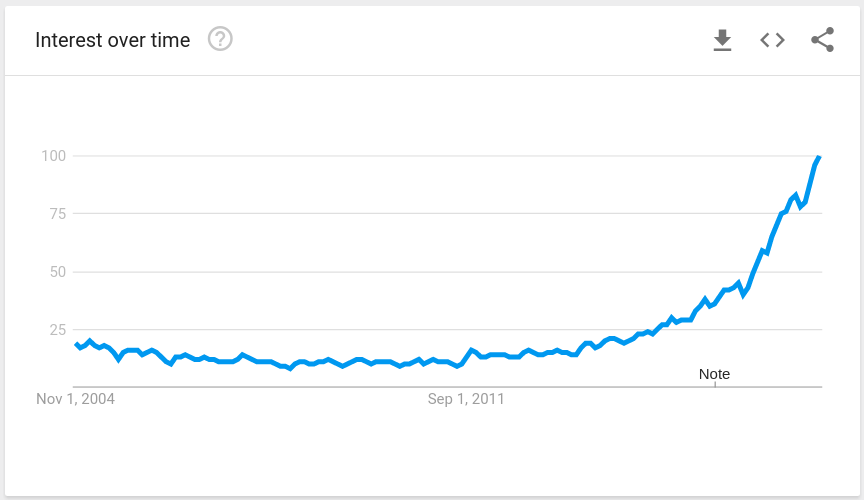
\includegraphics[width=0.6\textwidth]{figures/ml_trend.png}
      \caption{'Machine learning' Google search trend \cite{GoogleInc.2017}}
      \label{fig:ml_trend}
\end{figure}

The learning problem is summarized in Fig~\ref{fig:learning_problem} and follows the theoretical description provided at \cite{Yaser}. The learning algorithm \( \mathcal{A} \) receives data of any form, and its sole purpose is to identify mechanisms that describe that dataset \( \mathcal{D} \) closely. This dataset is defined as input-output samples for the supervised learning, input-weights samples for reinforcement learning and only inputs for the unsupervised learning. Further information regarding supervised, reinforcement and unsupervised learning can be found in section~\ref{ch:learning_types}. For the sake of the explanation, let us take the supervised learning case, where the dataset  \( \mathcal{D} \) includes samples of the form \((\mathbf{x}_1, y_1),\cdots , (\mathbf{x}_N, y_N) \), where \(x\) is the input that belongs to the input space \( \mathcal{X} \), \(y\) is the corresponding output such that \(y_n = f(x_n)\), and belongs to the output space \( \mathcal{Y}\). Now, the learning algorithm \( \mathcal{A} \) needs to find that function \(f(x)\). For this, it employs a hypothesis set \( \mathcal{H} \), which are the mathematical representations that the algorithm uses as tools to accomplish its purpose. From \( \mathcal{H} \) the algorithm takes one hypothesis \( g:\mathcal{ X \rightarrow Y} \) that approximates \(f\). After a \(g\) has been selected, the process estimates how alike the outputs from \(g(x)\) are to \(f(x)\), and feedbacks an error measure \(E(g,f)\). This process is repeated iteratively until a hypothesis produces an acceptable minimum error. \\

\begin{figure}[htb]
    \centering
      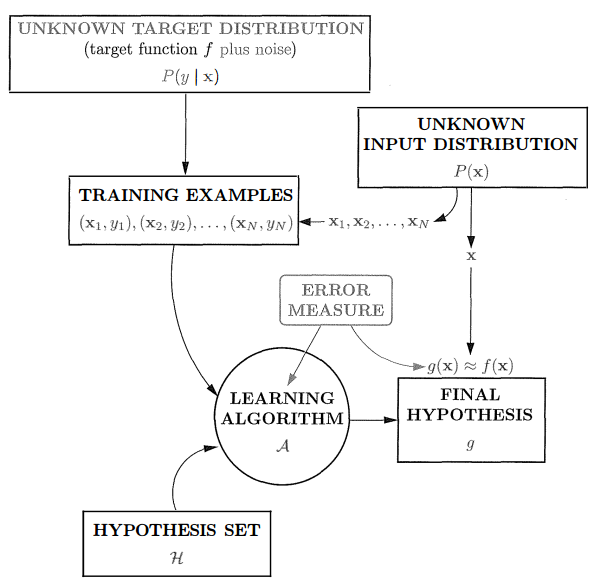
\includegraphics[width=0.6\textwidth]{figures/learning_problem.png}
      \caption{The learning problem \cite{Yaser}}
      \label{fig:learning_problem}
\end{figure}

Now, it is imperative to determine quantitatively what exactly \emph{acceptable} means. Different applications can have different tolerances to error, and this affects directly the hypothesis \( g \) that is chosen at the end of the learning process. This means that this is an end-user parameter that has to be set as a requirement for the whole system.

After taking different samples from \( \mathcal{X} \), and reducing the error, we should take into account the samples that \emph{we did not take}, meaning the samples that are not in our input set, and that probably behave similarly to the \( \mathcal{X} \) set - i.e. we should be able to identify similar samples in order to be able to predict. Therefore, a probability distribution is added to both the input samples and the final hypothesis in order to infer from \( \mathcal{D} \) the behavior of samples that are not in \( \mathcal{D} \). Let us assume a binary classification problem, where \( \mathcal{D} \) contains two classes, A and B, in a possibly infinite number. From a random sample pick the probability that the input sample is of the A type will be denoted as \(\mu\) and, consequently, the probability that the input sample is of the B type is 1 - \(\mu\). The value of \(\mu\) is unknown and will continue to be unknown in the process. From a random pick of N samples from \( \mathcal{D} \), there is a proportion of \(\nu\) samples of the A-type, and we intend to determine how \(\nu\) relates to \(\mu\). In statistical jargon, we want to determine how our sample relates to the whole population. \\

From any point of view, the larger the sample that contributes to \(\nu\), the closer the relation it has with \(\mu\), but this relationship can be quantified using the \emph{Hoeffding Inequality} \cite{Hoeffding1963}, which states that for any sample size \(N\),

\begin{equation}
  \mathbb{P}[|\nu -\mu|>\epsilon ]\leq 2e^{-2\epsilon^{2}N} \quad \text{for any}\quad \epsilon>0
\end{equation}

Where \(\mathbb{P}[\cdot]\) denotes the probability with respect to the chosen sample, and \(\epsilon\) can be any positive value chosen by the data scientist, and represents the tolerance of error. This inequality says, simply put, that as the sample size \(N\) grows, it is \emph{exponentially unlikely} that the realization \(\nu\) deviates from \(\mu\) by more than the tolerance \(\epsilon\). It can be clearly seen that only the size of the sample \(N\) affects this bound. Consequently, to achieve a small tolerance \(\epsilon\), a large \(N\) has to be used.\\

Additionally, it is important to take into account the intrinsic noise of the systems, which can come from the nature of the input samples, i.e the samples are not product of a deterministic system, or are immersed into some stochastic variation that can be modeled by noise, and that implies that by having the same input into the system \emph{it is probable} to get a different output. This entails a change in the labels of the model. That is, instead of having \(y = f(x)\), we take \(y\) as a random variable resulting from a probability distribution \(P(y|x)\). Accordingly, the input data points are therefore generated by the joint distribution \(P(x,y) = P(x)P(y|x)\). With this description of the model, our target function (what \(\mathcal{A}\) wants to learn) becomes \(P(y|x)\), while \(P(x)\) quantifies the importance of the input \(x\) in our learning accuracy.

\subsection{Types of learning}\label{ch:learning_types}

There are three types of learning: supervised-, unsupervised-, and reinforcement learning. Each of them has specific characteristics, which are explained in the following subsections.

\subsubsection{Supervised learning}
Is the type of learning where, in addition to the input dataset, the explicit correct outputs for those given inputs are given to the \ac{ML} algorithm for training. There are two types of supervised learning:
\begin{itemize}
    \item \textbf{Classification:} consists in predicting a \emph{class label} from a determined set of choices. If the number of choices is two, the model corresponds to a \emph{binary classification}. As it has only two options, it is suitable for the problems whose expected answer is of the form "yes/no", "present/not present", "valid/invalid". For a greater number of classes, the model corresponds to a \emph{multiclass classification}. \cite{Andreas} Provides a simple list of examples of classification:
        \begin{itemize}
            \item Determining whether an email is spam or not constitutes a binary classification problem.
            \item Identifying the zipcode from handwritten digits on an envelope is a multiclass classification problem.
            \item Determine whether a tumor is benign based on size and shape data constitutes a binary classification problem
        \end{itemize}
    \item \textbf{Regression:} consists in predicting a continuous behavior, such as a trend, or a floating-number, and it is this continuity what sets it apart from the classification models. Examples of regression \cite{Andreas} are:
        \begin{itemize}
            \item Predict the value of the stock market
            \item Determine the expected amount of crops yield from a plantation based on data such as previous yields, weather history, etc.
        \end{itemize}
\end{itemize}

\subsubsection{Unsupervised learning}
Unlike supervised learning, in unsupervised learning the algorithms are feed with data but not with the expected outputs, which make this type of learning suitable for solving problems to which the output is unknown. The model is then in charge of extracting knowledge from the input data all by itself, without no further instructions. There are mainly two types of unsupervised learning that can be found in the literature \cite{Andreas}, which are the \emph{unsupervised transformations} and \emph{clustering}.

\begin{itemize}
    \item \textbf{Unsupervised transformations:} consists in creating new representations of the input data, so that it becomes easier to understand and/or to use than the original data. This functionality is used, for example, to reduce the dimensionality of data that consists of several features. In such a situation, the model transforms the data into a representation that summarizes the input with fewer features. Another important use of this type of models is finding the overall representation of the input data, such as the topic of a full text, or the sentiment in a short comment.
    \item \textbf{Clustering:} this kind of models collects the data into determinate groups that share similar characteristics. This is used, for example, to generate suggestions based on previous purchases/views, or to group pictures from a directory with several images to the ones that contain certain people (and suggest tagging the names on them).
\end{itemize}

As the models do not know beforehand what type of information they are intended to learn, one of the tasks of the data scientist is to assess that the model is indeed learning something useful. This creates the opportunity for this sort of models to be used for the same data scientist to help them identify certain characteristics of the data that were not obvious for the \emph{human-eye}, and certainly get a different perspective of the data from the \ac{ML} model point-of-view.

\subsubsection{Reinforcement learning}
This type of learning has a different approach to the previous two descriptions. Just like unsupervised learning, the model does not receive the expected outputs for the inputs it is given but, in contrast, it receives some \emph{possible} output along with a weight that states how good of an output it is. The idea behind this is that the model is then penalized when it provides a solution that is not according to the possible output and is rewarded when it is. Then, the model uses these penalizations and rewards to adjust the type of outputs it generates, and so it eventually learns the correct behavior for the situations it has been immersed into. This type of learning is similar to the way humans learn, in ways such as being penalized with pain when taking a sip of very hot coffee, or rewarded when winning a game of chess.\\

In that same manner, reinforcement learning comes in handy in teaching an intelligent agent how to play a game, where it is presented to a plethora of options (which makes it difficult to be modeled as a supervised learning problem) and has to choose the one that brings it near to victory. The most recent example is AlphaGo \cite{Fu2017}, an intelligent agent capable of winning against the World Champion in a Go game. A similar approach has been followed by IBM with the Deep Blue chess-playing machine \cite{Hsu1999}.

\subsection{Training \& testing Models}
Training and testing are concepts that, when applied to learning algorithms, are not far away from the definitions that are used in common language when applied to humans. In general, \emph{training} a learning model consists of supplying it with enough data from which it can extract information and create generalizations, and testing consists of providing similar data to the model and identify if the generalizations apply. "Generalization" in this context means inferences, decisions or choices that the model makes on data it has never seen before based solely on the data it has learned from, and clearly, the goal of \ac{ML} is to have models that are able to generalize as accurately as possible. However, all learning scenarios depend on data, and this data, being as extensive as it can be, does not contain all the information that describes its surroundings completely. Therefore, the question arises: how can it be determined if the model can indeed learn to generalize from data?\\

The way to tackle this problem is separating the data into two: A portion of it to be used for training, and the rest of it to be used for validation/testing. Being the training set and testing set generated from the same whole dataset, it is expected that they share enough characteristics for the model to perform well at generalizing. However, there are cases when the model is too complex, and instead of learning to generalize it \emph{memorizes} the training set, and then performs poorly on the training set and on any unknown data. This phenomenon is known as \emph{overfitting} because the model is fit intimately to the training set as is not able to generalize on new data. That being said, one might think that creating the simplest learning model will never end up in overfitting, which is absolutely true. However, in such cases, the model might not be able to even capture the descriptive characteristics of the data, and ends up being incapable of learning from it. This phenomenon is known as \emph{underfitting}. Fig~\ref{fig:model_complexity} relates the complexity of the model with its capability of generalizing from new data.

\begin{figure}[!htb]
    \centering
      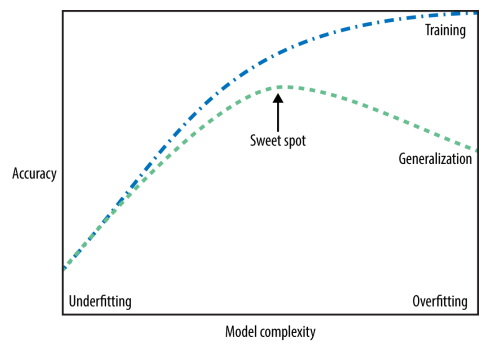
\includegraphics[width=0.6\textwidth]{figures/model_complexity}
      \caption{Model complexity vs. Training and test accuracy \cite{Andreas}}
      \label{fig:model_complexity}
\end{figure}

Therefore, it is clear that the objective model is not too simple or too complex, but somewhere in between; what \cite{Andreas} legitimately calls "the sweet spot", where the model has learnt as much as it can from the provided data, and is still able to create accurate inferences from unknown samples, ergo make predictions.


\subsection{Influence of dataset size in the learning process}\label{ch:size}
It has been constantly repeated that having data is paramount, but "how much data is required?" is a question that will always be asked, and that, unfortunately, has no concrete answer. The logic answer to it is "use as much data as possible", which also follows the Hoeffding inequality presented earlier in this chapter. Data is limited and generally comes along with the description of the problem itself. What this means is that, in data science, it is common for the learning problem to be stated as "The problem to solve is X, and the data available for it is Y" \cite{Yaser}. Asking for more data is, in most cases, impossible, and the data scientist has to work with what it has. However, the way the scientist extracts information from the data could be the lever that turns a failing model into a successful one.

Moreover, the model complexity is tied to the amount of information that the dataset holds; i.e. if the dataset has considerable variety within, the model can allow itself to grow in complexity without overfitting. This variety usually comes intrinsically with larger datasets, but the clarification has to be made: it is not the size of the dataset what directly yields to variety, meaning that duplicating samples won't help, as repeated data provides no increase on entropy.

\subsection{Data preprocessing}
Possibly the data that is measured or handed over to solve a problem does not provide much information \emph{as is}. However, after some careful treatment, that data might be transformed in the specific characteristics that allow an accurate generalization. The process of extracting specific \emph{features} that describe the information contained in the \emph{raw} dataset is called \emph{feature extraction}. It has been said earlier that unsupervised learning can be used for this purpose, using techniques such as \emph{Principal Component Analyzis (PCA)}, which retrives uncorrelated data and transforms the dataset component-wise in order to determine the information contribution of this component to the whole dataset. Other uses for unsupervised learning in data preprocessing are multiclass visualization, dimensionality reduction and generally finding a representation of the data that is more informative for later processing.\\

Additionally, feature extraction can be done manually, where the data scientist analyzes the data and produces a new dataset with a more representative description of it. This \emph{manual} method is also called \emph{feature engineering}, and was used by the \ac{CEL} in the DySpan spectrum challenge. Those extracted features are used in this work. A description of the implemented feature extraction process can be found in section~\ref{ch:features}.

Other type of preprocessing the data is \emph{scaling}, which comes in handy when samples of different orders of magnitude, belonging to different classes, are compared. This can be done, for example, by removing the mean of all the samples and scaling them to unit variance. Another way of scaling is setting a minimum and a maximum value, and fit all the features inside that range.

\subsection{Model Evaluation}
There are multiple ways to evaluate the performance of \ac{ML} algorithms, and they are helpful to determine if the model is generalizing from data satisfactorily. In this work, we focus on multiclass classification, and one of the most thorough tools for model evaluation is the confusion matrix. When a confusion matrix is calculated for a multiclass classification problem, a square matrix with dimensions equal to the number of classes is generated. Fig~\ref{fig:conf_matrix} shows the confusion matrix configuration for a binary classification, where the classes are "positive" and "negative". Each cell of the matrix contains the number of samples from the testing set that was classified to that specific class. This means that the diagonal of the matrix states the number of correctly classified elements.

\begin{figure}[htb]
    \centering
      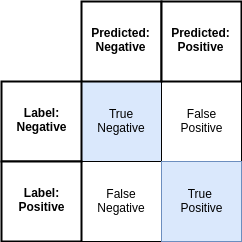
\includegraphics[width=0.4\textwidth]{figures/cm}
      \caption{Confusion Matrix}
      \label{fig:conf_matrix}
\end{figure}

Some applications have to regard specifically the type of misclassification that could happen in order to focus efforts into mitigating it. Prof. Yaser \cite{Yaser} exemplifies this with a fraudulent credit card transaction. If a fraudulent transaction is not happening, meaning that the rightful owner of the credit card is make use of the services he/she is entitled to, but the transaction is labeled as fraudulent, this has little negative consequences when compared with the situation in which a fraudulent transaction is indeed happening but is labeled as an honest one.

In this work, misclassification affects equaly the final output regardless of its type.
\subsection{\ac{ML} algorithms}\label{ch:ml_algs}
\subsubsection{K-nearest Neighbors}
This is one of the simplest \ac{ML} algorithms, and consists solely of making decisions based on the characteristics of the points that surround the point under test, i.e. the "nearest neighbors". It can be used for both supervised and unsupervised classification as well as for regression. The distance with which the "nearest" point is determined can be any metric measure such as:
\begin{itemize}
    \item Euclidian distance between any two points \( \sqrt{\sum (x - y)^2} \)
    \item Manhattan distance \( \sum {|x - y|} \)
    \item Chebyshev distance \( max(|x - y|) \)
    \item Minkowski distance \( \sum(|x - y|^p)^{1/p} \)
\end{itemize}
among others.

This algorithm is commonly called \emph{non-generalizing} because it remembers the location of its training data points and checks the proximity of its points to every other new data to predict. However, even though this procedure seems as "memorizing", this algorithm is not prone to overfitting and can lead to satisfactory results in datasets of various sizes, and because of its easiness to understand and apply, it is a good choice as a starting point for tackling a learning problem before applying more elaborated models. On very large datasets, or on datasets of very high dimensionality (several hundreds of classes) the amount of distances calculations escalates, which might lead to long prediction times.

\subsubsection{Decision trees}
This model is based on simple boolean-like bifurcations (if-then) that build a hierarchy tree that eventually leads to a decision, which makes it an uncomplicated model easy applicable in classification and regression. The concept can be easily explained with an example: assume that we have four common elements that can be found in a lab, such as an external monitor/screen, a laptop, an office chair and a USB stick. The classification of such can be as simple as it is shown in Fig~\ref{fig:dt_example}. In this example, the features are "has a screen?", "has wheels?" and "has a keyboard?". Clearly, this example model can be extended for further classification of lab elements.

\begin{figure}[!htb]
    \centering
      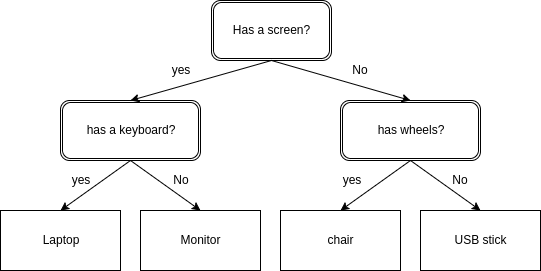
\includegraphics[width=0.7\textwidth]{figures/dt_example}
      \caption{Decision tree for classification of four lab elements}
      \label{fig:dt_example}
\end{figure}

The complexity of the model is given by the number of questions that have to be asked before reaching a final decision, i.e. the depth of the tree. With a long depth, the questions become more specific, and only a few samples are able to fit the tree, which leads to overfitting. In \ac{ML}, the tree is generated automatically, so a good way to avoid overfitting is stopping the tree from growing more than it should, in a process called \emph{pre-pruning}, or removing branches that provide little to no information after the tree has been created, which is called \emph{post-pruning}.

Given the nature of the decision tree, preprocessing the data (with methods such as scaling) does not influence its performance in terms of accuracy, because each feature is processed completely independent of the others. Because of this reason, this model is recommended when the features do not fall into a common range or have completely different characteristics (such as a mixture of discontinuous and continuous features).

\subsubsection{Support Vector Machines}
Support vector machines (SVM) are an extension of the linear models that serve as a base for classification systems, such as the perceptron, which is explained more in detail in section~\ref{ch:neural}. Basic linear models are not regarded in this work because they are not explicitly used in the implementation described in following chapters, and the specifics of the mathematic description for the linear models and \ac{SVM} models is extensive and out of the scope of this thesis. Prof. Yaser provides an extensive explanation of perceptrons and on its use for the learning process \cite{Yaser}. In summary, a linear model sets a classification boundary that separates different classes. \ac{SVM} extends this functionality by introducing the concept of \emph{hyperplanes}, which ensures an improved classification by maximizing the separation of points of different classes by the means of the hyperplanes. This classification boundaries are shown in Fig~\ref{fig:svm} for two different classes.

\begin{figure}[!htb]
    \centering
      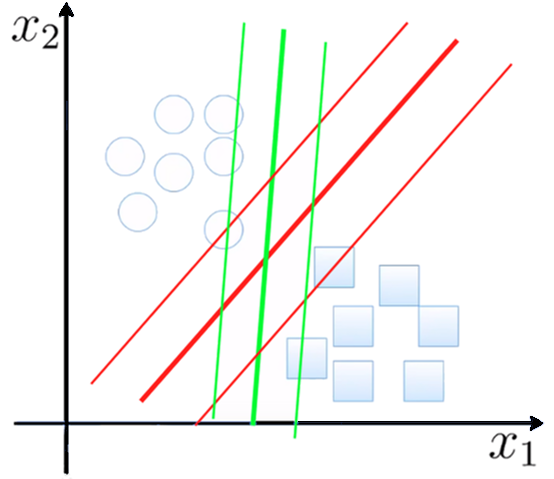
\includegraphics[width=0.5\textwidth]{figures/svm}
      \caption{\ac{SVM} - Hyperplanes separating two classes. Functional margin in red.}
      \label{fig:svm}
\end{figure}
The hyperplanes that generate the largest separation between training data points of different classes form a so-called \emph{functional margin}, which provides the smallest generalization error for the classifier. These models are said to have exceptionally good performance in high dimensional spaces, even when the number of classes is greater than the number of available samples \cite{SKLEARN}.

\section{Deep Learning}
Additionally, to the approach of learning from extracted features, deep learning is an approach based on learning data representations. This is a subgroup of \ac{ML} and was developed on top of a technique called Neural Networks, which is described briefly below. The term "Deep learning" was coined in 1986 by Rina Dechter \cite{Dechter}, in a proposed work to overcome a way to learn the maximum amount of information from techniques using backpropagation, making a parallel of learning and recording, and so when a so-called \emph{dead end} is encountered, the recorded information could guide iteratively to make new decisions.

\subsection{Neural Networks}\label{ch:neural}
Before getting deeper into the specifics of neural networks, it is precise to first define one small unit that is used to build the networks: the perceptron. A perceptron is a node that implements a very simple binomial linear classification. It maps the output based on an activation function applied to the input:

\begin{equation}
    f(x) =
    \begin{cases}
        1 \text{ if } w*x + b > 0\\
        0 \text{ otherwise}
    \end{cases}
\end{equation}

It can clearly be seen that the output of the perceptron is based on a linear equation of the form \(y=mx+b\), where \(w\) is a vector of weights, \(x\) is the input of the perceptron, and \(b\) is the bias. The weights set certain restrictions to the input data, and the bias determinates the decision threshold for a binary classification. Assuming that values higher than the threshold are set to a positive decision, and below the threshold to a negative decision, the mathematic representation is set as:

\begin{equation}
    \text{positive decision if } \sum_{i=1}^{d} w_i\cdot x_i > \text{bias}
\end{equation}
\begin{equation}
    \text{negative decision if } \sum_{i=1}^{d} w_i\cdot x_i < \text{bias}
\end{equation}

which can be represented in the following simplified form:
\begin{equation}
    \text{decision } h(x) = \text{sign}\left(  \left( \sum_{i=1}^{d} w_i\cdot x_i \right )+ b \right )
\end{equation}

A basic representation of a perceptron is shown in Fig~\ref{fig:perceptron}.

\begin{figure}[!htb]
    \centering
      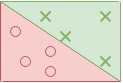
\includegraphics[width=0.4\textwidth]{figures/perceptron}
      \caption{Interconnection of perceptrons generating a simple neural network. \cite{Yaser}}
      \label{fig:perceptron}
\end{figure}

Perceptrons are also called \emph{neurons}, which are activated to specific types of input data. When more neurons are interconnected, each one with a different activation function (based on the weights and the bias), a neural network is created, which can then classify input data of higher complexity. An arbitrary amount of neurons can be added increasing as well the complexity of the network, but each of them classifies the data independently. Historically, the name \emph{neural network} is given because of the similarity of this behavior to the synapses of the neurons in a biological neural system. The book of professor Yaser \cite{Yaser} explains in further detail the perceptrons and the learning process using these units.

\begin{figure}[!htb]
    \centering
      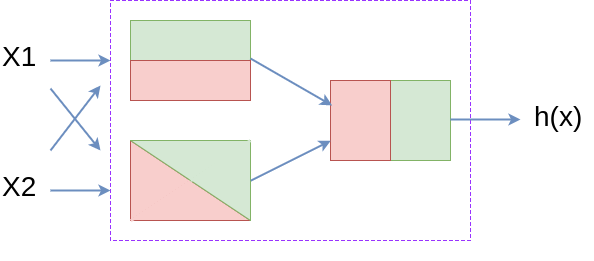
\includegraphics[width=0.8\textwidth]{figures/neuralnetwork}
      \caption{Basic structure of a neural network.}
      \label{fig:neuralnetwork}
\end{figure}

\subsection{Convolutional Neural Networks}

\ac{ConvNet} are a special type of neural networks that share their parameters across space, making them suitable for image classification. The main idea is as follows: assume we have an image depicted in blue in Fig~\ref{fig:convolutionalnetwork} as the input of this system, whose dimensions are (height, width, and depth). The height and width are the numbers of pixels that determine the size of the picture, and the depth is 3 for color pictures (RGB) and 1 for grayscale. When this picture is inserted into the \ac{ConvNet}, only a portion of it is regarded as a so called patch, shown in red.

\begin{figure}[t!]
    \centering
      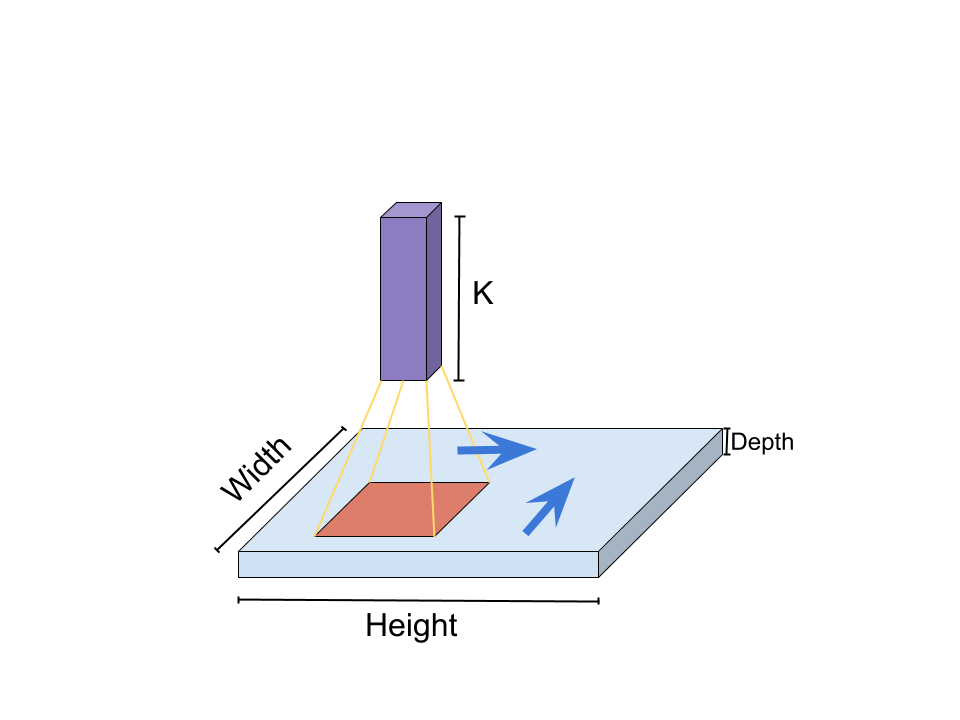
\includegraphics[width=\textwidth]{figures/convolutionalnetwork}
      \caption{Convolutional Network}
      \label{fig:convolutionalnetwork}
\end{figure}

This patch, also called kernel, is then swept along the picture with a given arbitrary stepsize, applying a neural network operation over it. As it is a smaller patch, each operation regards many fewer weights in comparison with the whole input, which is shared across space with the slide operation. As a result, a stack of convolutions is generated, representing a picture-like output, having not only a reduced height and width but an increased depth K that represents the non-linearities that describe the input, as if it increased the number of color channels that describe the input picture.\\

Generally, these convolutional layers are stacked together generating a pyramid, in a so-called sequential model, reducing the spatial dimensions of an input image (h,w), but increasing its depth. As a result, the depth corresponds to the \emph{semantic complexity} of the image representation, mapping the illustrative content of it. Inside of each layer, there is a number K of filters, in charge of picking different characteristics from the image, such as a specific shape or a determinate intensity value. The characteristic that the filter notices is not programmed, but learned by itself. This means that the network learns on its own what type of feature representation is going to learn and, consequently, which shape is going to activate it.



  \acresetall
\chapter{Testbed Implementation}\label{chapter:implementation}\label{ch:implementation}
This chapter depicts the tools and procedures used in the setup and data preparation prior to the application of \ac{ML} algorithms. First, an overview of the software and hardware tools is given. Afterwards, a short explanation on the available \ac{ML} libraries and frameworks is presented, along with the reasoning behind their choice for this work. Lastly, the process of recording the data and preprocessing it is explained in detail, for the data to be ready to be applied to the learning models.
\section{Development Tools}\label{ch:tools}
As stated in the introduction of this thesis, \ac{SDR} and \ac{CR} play an important role in modern communication systems and is the framework used for most projects at the \ac{CEL}, not only being used as a tool but also being actively contributed to with research results, but also acting as an active agent on open-source improvements. The software and hardware frameworks used are the following:
\subsection{GNU Radio}
\begin{figure}[htb]
    \centering
      
\includegraphics[width=0.8\textwidth]{figures/gnuradio_logo}
      \caption{GNU Radio logo}
      \label{fig:gnuradio}
\end{figure}
GNU Radio \cite{GNURadio2016} is a free and open-source toolkit that provides a large library of signal processing blocks that can be used for several software-defined radio applications. Its functionality does not require a physical device in the loop, which allows the users to simulate complete communications systems only on a computer. This includes signal sources, modulators and demodulators (such as \ac{PSK} and even \ac{OFDM}), dynamic channel simulators (and virtually any digital filter implementation), math operators, and a plethora of other digital signal processing implementations that have served purposes in the academy, research, amateur radio hobbyist and even some government entities. Additionally, thanks to the support for several \ac{SDR} devices \cite{gnuradiohw}, GNU Radio grants the capability of transmitting a generated signal (given the user has a rightful license for this purpose) and/or receiving real signals and decode them.\\

The usual usage of this software is as follows: the user has a problem or an idea that requires digital signal processing, such as decoding a radio signal or implementing a novel communications' protocol. As said, GNU Radio includes several algorithms that serve this purpose, and they are enclosed in so-called blocks. These blocks can then be connected to one another, generating a flow that the signal follows, in a so-called flowgraph, where each block takes a determinate amount of inputs, each input also taking a determinate amount of samples, that undergo the signal processing that the block describes, and then the block presents its outputs to the next block downstream. If the library provided by GNU Radio does not contain implementations that suffice the user needs, new implementations are easily added by the means of a so-called \emph{\ac{OOT}} module, where the user can provide additional applications and characteristics that make the scalability of GNU Radio a transparent procedure. Lastly, if the user believes that custom implementation can serve a common purpose and other users, the \ac{OOT} can be made public following the open source standards, and this way other users can benefit from the same implementation and probably even contribute to it. An extensive collection of \ac{OOT} that have followed this open source mentality can be found at \ac{CGRAN} \cite{CGRAN}.\\

Regardless of the number of inputs and outputs on a block, the amount of items required for the algorithm within determines its type:

\begin{itemize}
    \item If for each output produced the block requires only one input item (1:1), then it is a \emph{sync} block.
    \item If the block requires N input items in order to generate 1 output item (N:1), the block is a \emph{decimation} block.
    \item If the block generates M output items for each 1 input item (1:M), the block is an \emph{interpolation} block.
    \item If the block requires extended flexibility, requiring N input items for each M output items produced (N:M), the block is a \emph{general} block.
\end{itemize}

Most of the blocks are written in a parametrizable fashion, serving multiple purposes with the same implementation by allowing the user to set different settings which can go from the general point of view, such as the vector length of the signal and its data type, to very specific and detailed parameters such as the taps of a filter or the description of a preamble. \\

The library of algorithms is organized in modules that have a common purpose, and within these modules, you find blocks that help achieve that purpose. Examples of such modules are the “gr-qt” module contains the blocks that are intended to be used for visualization purposes using Qt \cite{Qt} and, within this module, blocks such as a “Time sink” and a “Frequency Sink” are found, which are written using Qt and serve as a scope and as a spectrum analyzer, respectively. Another example, more specific, is the gr-channels module, where the user can find different implementations for parametrizable channel simulators, such as fading, frequency selective, and dynamic channel models, among others. Most of these blocks are written in C++ and python, where each block is, in end effect, a class. In the same programming jargon, the module is a namespace. Therefore, the end user is expected to feel comfortable understanding (and, optimally, using-/writing-) these programming languages in order to be able to use these blocks to the fullest. The interconnection of the blocks, i.e. the flowgraph, is written using Python. For the C++ blocks to be available in the Python interface of the flowgraph, this C++ implementation is translated into Python domain by making use of the \emph{\ac{SWIG}}. In addition, multiple blocks can be grouped into a single block that serves a specific purpose, and this is called a hierarchical block.\\

Although coding to the base of the modules and blocks gives the user total control of the details, it is not the only way of getting things done while using GNU Radio. The software comes with a \ac{GUI} called \ac{GRC}, which allows the user to drag-and-drop blocks into a canvas and connect them directly with the ease of a click. Even experienced users grab a hold on this \ac{GUI} as it provides ease and versatility along with a visible flowgraph that is easy to understand not only for the user but also to other users whose interest has been drawn to a specific application.\\

Additionally, GNU Radio features the \ac{VOLK}\cite{VOLK}, a free library of hand-written SIMD mathematical operations used to handle vectorization efficiently. This library is used in this work to optimize operations in the spectrogram generation process, described in section~\ref{ch:spectrogram}.\\

In order to use GNU Radio, the recommended installation is done by the means of \ac{PyBOMBS} \cite{PyBOMBS}, which also allows installation of the modules listed in \ac{CGRAN}.

\subsection{Universal Software Radio Peripheral}
\begin{figure}[htb]
    \centering
      
\includegraphics[width=0.5\textwidth]{figures/ettus_logo}
      \caption{Ettus Research's logo}
      \label{fig:ettus}
\end{figure}

One of the \ac{SDR} devices that are supported by GNU Radio is the \ac{USRP}, which is developed and produced by the company \emph{Ettus Research\texttrademark} \cite{Ettus}. This company has been one of the most representative suppliers of \ac{SDR} devices around the globe, and these devices are renowned by its outstanding performance and versatility.\\

During the complete \ac{DySpan} spectrum challenge competition, three different \ac{USRP} devices where used for both \ac{PU} and \ac{SU}. The \ac{PU} used for the transmitter and the receiver the \ac{USRP} X310, which can be seen in Fig.~\ref{fig:x300} \cite{X300}. This device has two wide-\ac{BW} \ac{RF} daughterboard slots and a large customizable Xilinx Kintex-7 FPGA. Additionally, it has the capability of using high-speed interfaces such as 10gigE and PCIe, with which a maximum of 200MS/s full duplex can be travel through the transport link. This \ac{USRP} covers from 10MHz until 6GHz, but based on the daughterboard selected, which serves as \ac{RF} frontend, the frequency of operation of the device can vary.\\

As for the \ac{SU} that was presented by the \ac{KIT} \ac{CEL} group, the transmitter used a \ac{USRP} N210, depicted in Fig~\ref{fig:n210} \cite{N210}. The N210 has a Xilinx Spartan 3A-DSP 3400 FPGA and supports up to 100MS/s through a 1gigE link that connects it to a host machine.  This device also requires an \ac{RF} daughterboard as a frontend, for which in the \ac{SU} implementation the UBX-40, shown in Fig~\ref{fig:UBX} \cite{UBX}, was used. This daughterboard can operate from 10MHz to 6GHz, providing an instantaneous \ac{BW} of 40MHz. As for the receiver, a B210, shown in Fig~\ref{fig:b210} \cite{B210}, was used. This \ac{USRP} is a fully integrated, two-channel device that operates from 70MHz to 6GHz without the need of additional \ac{RF} frontend configuration. It provides full duplex, MIMO (2 Tx - 2Rx) operation up to 56 MHz of instantaneous \ac{BW}. Furthermore, it counts with a convenient USB 3.0 connection that also serves as the power feed.\\

Although these devices provide high-end performance and its versatility is outstanding, \ac{USRP} such as the B210 has still a very competitive price for the quality of its elements. Additionally, Ettus Research\texttrademark is committed to the Open Source community by making its source code available for developers that want to either have a look at it, modify it to add specific functionalities to the \ac{USRP} devices or contribute to it.

The interface between the devices and the host machine is performed by the \emph{\ac{UHD}}, an open-source software driver provided by Ettus Research\texttrademark that furnish support for all \ac{USRP} devices. This driver supplies API for usage of \ac{USRP} devices as stand-alone, and also provides support for GNU Radio via the gr-uhd \ac{OOT}.

\begin{figure}[htb]
    \centering
    \begin{subfigure}[htb]{0.45\textwidth}
        \centering
        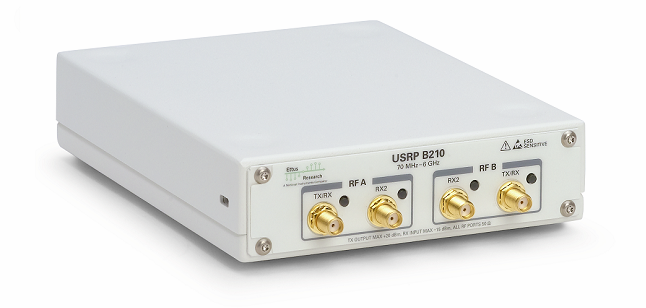
\includegraphics[width=0.7\linewidth]{figures/b210}
        \caption{USRP B210\cite{B210}}
        \label{fig:b210}
    \end{subfigure}
    \begin{subfigure}[htb]{0.45\textwidth}
        \centering
        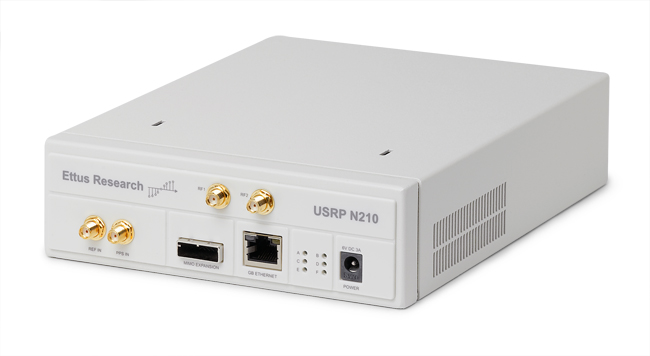
\includegraphics[width=0.7\linewidth]{figures/n210}
        \caption{USRP N210\cite{N210}}
        \label{fig:n210}
    \end{subfigure}
    \begin{subfigure}[htb]{0.5\textwidth}
        \centering
        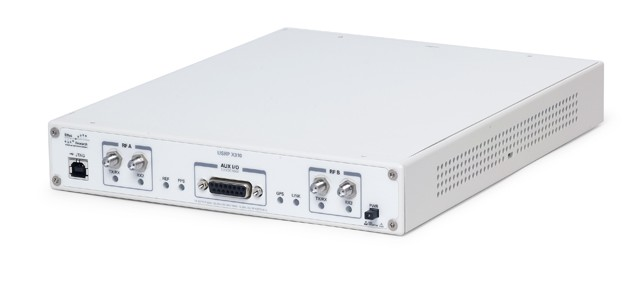
\includegraphics[width=0.7\linewidth]{figures/x310}
        \caption{USRP X300\cite{X300}}
        \label{fig:x300}
    \end{subfigure}
    \begin{subfigure}[htb]{0.4\textwidth}
        \centering
        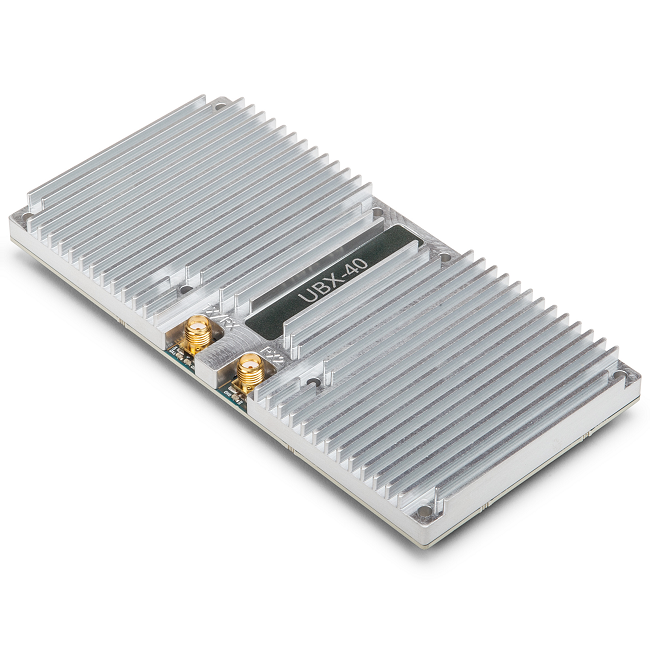
\includegraphics[width=0.6\linewidth]{figures/UBX40}
        \caption{UBX-40 daughterboard\cite{UBX}}
        \label{fig:UBX}
    \end{subfigure}
    \caption{\ac{USRP} Devices used in the complete DySpan challenge setup}
    \label{fig:ettus}
\end{figure}

For this thesis, the \ac{SU} implementation is reproduced, for which the N210 as transmitter and the B210 as receiver are used.

\section{\ac{ML} models in Python and Jupyter}
\begin{figure}[!h]
    \centering
    \begin{subfigure}[htb]{0.45\textwidth}
        \centering
        
\includegraphics[width=\linewidth]{figures/python_logo}
        \label{fig:python}
    \end{subfigure}
    \begin{subfigure}[htb]{0.45\textwidth}
        \centering
        
\includegraphics[width=\linewidth]{figures/jupyter_logo}
        \label{fig:jupyter}
    \end{subfigure}
    \caption{Python and Jupyter logos}
    \label{fig:python_jupyter}
\end{figure}
For the \ac{ML} part of this work, the focus on the implementation was given to a couple of popular Python libraries that have been effective when dealing with \ac{ML} problems: scikit-learn \cite{SKLEARN} and keras \cite{KERAS}. These libraries were chosen because of the simplicity of their prototyping as well as their effectiveness when providing an implementation that suits the \ac{ML} needs by returning fully trained models with exceptional prediction accuracy, and are described in more detail in the following sections. Additionally, the fact that these libraries are written in Python raises interest because this means that they interface optimally with GNU Radio, making the inclusion of these libraries transparent, and having the perks of Python such as easy debugging and extensibility.\\

As for model testing and visualization, Jupyter notebooks \cite{Jupyter} have been used and are presented as part of the code repository of this thesis. What Jupyter provides is an open-source web application in which a number of interpreters for languages such as Python, R, Julia and Scala are embedded, allowing the creation and sharing of an interactive register that contains code lines and execution output along with visualization fields for plots and graphs and documentation in markdown, in what is called \emph{literate programming}. These notebooks can be shared in multiple formats, such as the native notebook format (for further modification of its contents), as well as HTML, \LaTeX{} and PDF (generated with \LaTeX). Moreover, it is nicely integrated with GitHub, so that the notebook can be visualized in the webpage of a remote repository without the need of conversion.\\

Jupyter is the continuation of a long effort for supporting interactive Python interpreters - the IPython Project \cite{IPython}. It has had a massive adoption in the last few years, such that even complete books have been written only using Jupyter as their interface for text editing and code examples. One of the main sources used for this work \cite{Andreas} is an example of such.

\subsection{Scikit-learn}
\begin{figure}[!ht]
    \centering
    
\includegraphics[width=0.4\linewidth]{figures/sklearn_logo}
    \caption{Scikit-learn logo}
    \label{fig:sklearn_logo}
\end{figure}
Scikit-learn, formerly scikits.learn and also known as sklearn, is \ac{ML} library that features an abundance of algorithms for supervised and unsupervised algorithms, including the ones described in section~\ref{ch:ml_algs}. This library came as a result of a \emph{Google Summer of Code} project as a third party extension to SciPy, from where it gets its name. This library was used in this thesis for all the learning based on the extracted features listed in section~\ref{ch:features}.

\subsection{Keras}
\begin{figure}[!ht]
    \centering
    
\includegraphics[width=0.5\linewidth]{figures/keras_logo}
    \caption{Keras logo}
    \label{fig:keras_logo}
\end{figure}
Keras is a high-level neural networks API written in Python that uses TensorFlow \cite{TensorFlow}, CNTK \cite{CNTK} or Theano \cite{Theano} as a backend. The way it is written allows data scientist to prototype and experiment fast. As per its documentation \cite{KERAS}:\emph{"being able to go from idea to result with the least possible delay is key to doing good research"}, and Keras certainly intends to keep the coding part as simple as possible for the designer to focus on the idea and not the programming of it. For this, it presents and API that is:

\begin{itemize}
    \item User-friendly: with ease of writing, reading, and understanding.
    \item Modular: models have a clear begin and end, and they can be easily connected with other models with low to no restrictions.
    \item Extensible: new functionalities and features are easily added to the mainstream, and the existing codebase is well-documented and exemplified.
\end{itemize}

For this project, Keras is used for the convolutional neural networks implementation, using Tensorflow (with GPU support) as a backend.

\section{Setting up the development environment}
This thesis was completely done using Linux-based operating systems, and the steps depicted below have been tested on Fedora 25 as well as on Ubuntu 16.04LTS. Installation in other Linux distributions have small to no difference from these steps. For the setup on a machine using Microsoft Windows\texttrademark, please refer to the documentation of each of the tools listed in section~\ref{ch:tools}.\\

For GNU Radio and \ac{UHD}, \ac{PyBOMBS} was used because of the ease it provides on installation, as well as the capability of installing the software in a self-contained environment that does not pollute the system domain. However, installation by source can also be performed, and a very detailed sequence of steps can be found in the following for Linux \cite{Linux}, MacOS \cite{OSX} or Windows \cite{Windows}. First of all, \ac{PyBOMBS} needs to be installed, and the recommended way to do so is by using \ac{pip} which, as well, is the recommended way to install Python packages.  Installation is simply done by running the following command, which will download the latest release:

\begin{lstlisting}
    $ [sudo] pip install PyBOMBS
\end{lstlisting}

In order to install the latest version from the git repository, the following slight modification to that command is needed:

\textbf{NOTE:} along this work, only Python2 was used because of compatibility with the current master branch of GNU Radio. Future work includes porting this work onto the Py3k improvements of GNU Radio, along with newer versions of the following installed libraries.

\begin{lstlisting}[breaklines=true]
    $ [sudo] pip install [--upgrade] git+https://github.com/gnuradio/pybombs.git
\end{lstlisting}

Now, there is an option for \ac{PyBOMBS} to parse the best possible configuration specific to the development machine (such as amount of threads used for package installing and a git-cache that speeds up repeatable git clones). This configuration is set up as follows:

\begin{lstlisting}[breaklines=true]
    $ pybombs auto-config
\end{lstlisting}

\ac{PyBOMBS} uses so-called recipes that contain the software description as well as its dependencies. This makes possible to automatically generate dependency trees, that will be automatically installed when a package requires them. The recipes are downloaded and installed as follows:

\begin{lstlisting}[breaklines=true]
    $ pybombs recipes add-defaults
\end{lstlisting}

Up to this point, \ac{PyBOMBS} has the references necessary to install GNU Radio and \ac{UHD}, and it is only needed to specify where in the development machine this software is to be located. For it, we generate a self-contained prefix, which allows us to keep the software all in one place without polluting the system domain. The next command creates a folder called "workarea" in the home directory: {\raise.17ex\hbox{$\scriptstyle\sim$}}\textbackslash workarea, gives it the alias "workarea" (which will help \ac{PyBOMBS} identify this prefix uniquely) and will start the GNU Radio installation after installing all its dependencies, \ac{UHD} included:

\begin{lstlisting}[breaklines=true]
    $ pybombs prefix init ~/workarea -a workarea -R gnuradio-default
\end{lstlisting}


In order to install the \ac{ML} libraries, there are multiple options as well. The libraries can be installed using pip with the following command:

\begin{lstlisting}[breaklines=true]
    $ [sudo] pip install numpy scipy pandas graphviz jupyter scikit-learn tensorflow keras
\end{lstlisting}

Numpy and Scipy should have been installed during the GNU Radio installation, but are listed in the command for completeness' sake. It is also recommended installing this tools in a dedicated Python Environment, such as Conda or Virtualenv. Procedures on how to generate these virtual environments, and already saved environments that can be pulled and installed (included the versions used in this work) are included in the GitHub repository of this thesis \cite{repo:cognitive_radio_ml}.

\textbf{NOTE:} For training using Keras/Tensorflow, and given that the development machine has a compatible graphics card, it is recommended to install Tensorflow with GPU support. By doing so, the training times are reduced drastically. This work was developed and written using a Lenovo Thinkpad W541, which has an NVIDIA Quadro K2100M Graphic card, compatible with CUDA. For this dedicated installation, a combined procedure from \cite{Yadak} and \cite{Andrews} was used.

\section{Dataset Generation}
This part of the work regards the steps taken in order to have the data ready for the \ac{ML} algorithms to learn from it. It covers the testbed setup, the raw data (I/Q samples) measurement, and the data preprocessing.
\subsection{Measurement Campaign}\label{ch:measure}
The first step taken was to set up the \ac{PU} communication link over the air, and recording the raw samples just as the \ac{SU} would be able to "hear" them. The measurement setup is shown in Fig~\ref{fig:measurement}, where two parts are labeled separately.

\begin{figure}[!htb]
    \centering
    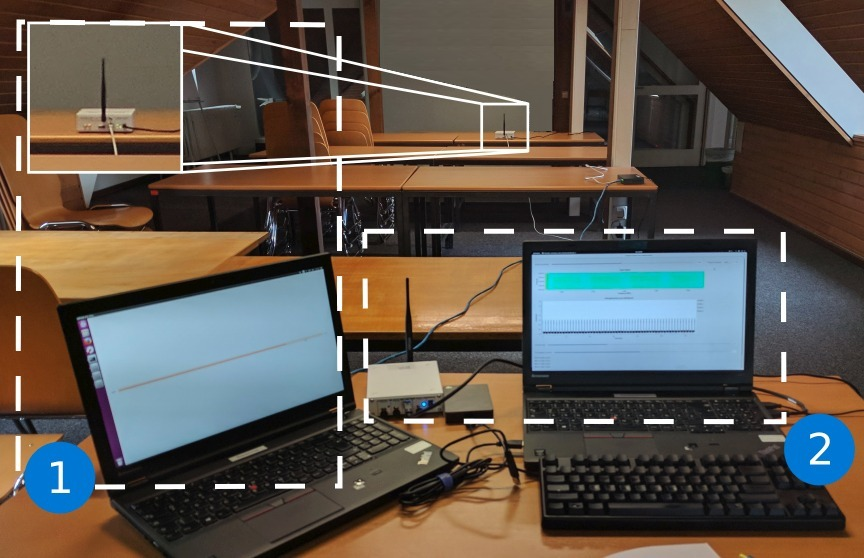
\includegraphics[width=0.5\linewidth]{figures/mod}
    \caption{Measurement Setup}
    \label{fig:measurement}
\end{figure}

The part labeled with \raisebox{.5pt}{\textcircled{\raisebox{-0.9pt} {1}}} regards the transmission part, which is sending frames over the air in ten different fashions, described in Table~\ref{table:scenarios}.  The host machine in this part has the connection to the database, from where the information frames are extracted and put as the payload of the transmitted frames. Additionally, the GNU Radio flowgraph that generates the signal, which can be seen in Fig~\ref{fig:PU_flowgraph}, is also hosted and run on this computer. A summary of the path that a frame travels from the database until the transmitter is as follows: in Fig.~\ref{fig:PU_flowgraph} it can be seen that a connection to the database is done in the "Cmd pktgen" block, which is in charge of retrieving the information frames from the database, in form of \ac{PDU}, and feeding them into the signal processing blocks. After converting the \ac{PDU} into a byte tagged stream (a stream of data that has metadata attached to it in form of tags), the stream flows into the \ac{OFDM} transmitter block, which is a hierarchical block that allocates the carriers for an \ac{OFDM} transmission, applies a \ac{FFT} to them, and appends a cyclic prefix.

Right after, the output, which is a complex I/Q tagged stream, is then converted again into \ac{PDU} and feed into the packet controller block. This block is in charge of generating the different scenarios that are set to be identified in this thesis by the means of learning techniques. The parameters of this block are not modified along this work, except one: the "scenarios list". By setting the scenario list to a specific value from 0 to 9, a determinate behavior can be set and recorded, and when this samples (after the feature extraction of section~\ref{ch:features}) are paired to the selected scenario, they have the form (input, output), suitable for supervised learning techniques. The rest of the flowgraph, consistent of resampling and multiplying with a sine signal, corresponds to a traditional mixing to the specific channels between the 10MHz \ac{BW} centered at 3.195GHz. As for the \ac{RF} frontend, an N210 \ac{USRP} was used, which in the flowgraph is represented as the "UHD:USRP sink" block.

\begin{figure}[!htb]
    \centering
    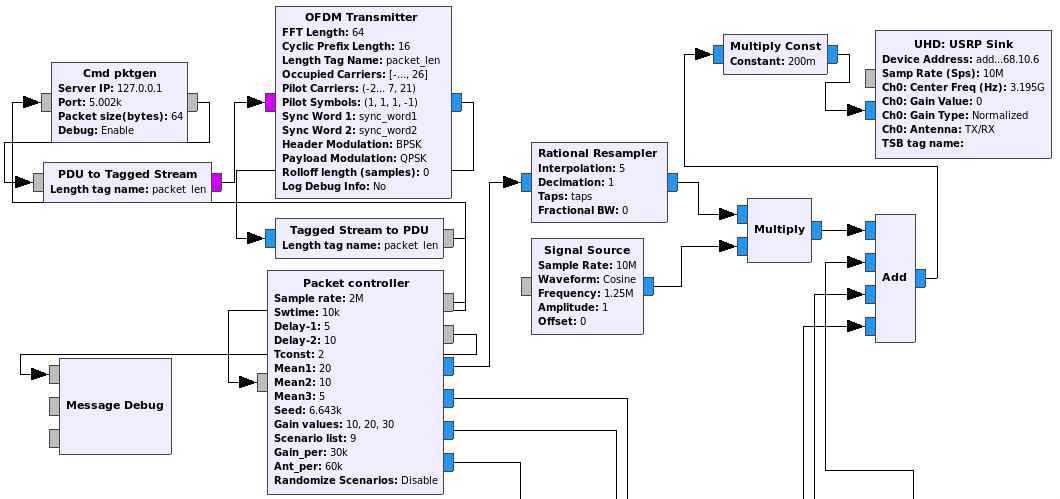
\includegraphics[width=\textwidth]{figures/PU_flowgraph}
    \caption{Portion of the \ac{PU} GNU Radio flowgraph}
    \label{fig:PU_flowgraph}
\end{figure}

The part of Fig~\ref{fig:measurement} labeled with \raisebox{.5pt}{\textcircled{\raisebox{-0.9pt} {2}}} corresponds to the recording system. In this machine, a very simple flowgraph has been implemented and is shown in Fig~\ref{fig:recording_flowgraph}. A "UHD: USRP source" block, which in real life is an \ac{USRP} B210, is connected directly to a couple of scopes: A Waterfall sink and a Time Sink. These scopes, however, are only used for supervision of the presence of energy over the air and have no effect whatsoever on the recorded signal. The main path is then the "File sink", which directly saves the data presented at its input into a file and the "Head block" which serves as a gauge to limit the amount of data that is saved to disk. Taking disk space into consideration, it was decided to record 1 minute of raw samples per scenario: 30 seconds with the presence of DC offset in the transmitter, 30 seconds without it. The DC offset is taken into consideration because the assumption is made that there is no strict control on how the \ac{PU} transmission is made apart from the specs given, so this is an attempt to cover every possible situation. The reason behind this time limitation is the amount of data that has to be taken into consideration. The math behind it is as follows:
\begin{equation}
    \frac{\SI{10}{\mega S}}{\SI{1}{s}} \cdot \SI{60}{s} \cdot \frac{\SI{8}{\byte}}{\SI{1}{S}} = \SI{4.8}{\giga\byte}
\end{equation}

\begin{figure}[!htb]
    \centering
    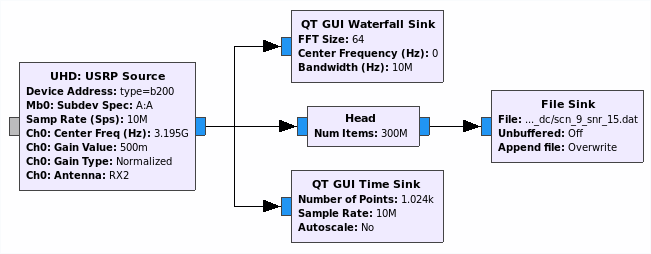
\includegraphics[width=\textwidth]{figures/recording_flowgraph}
    \caption{Flowgraph used to record over-the-air samples}
    \label{fig:recording_flowgraph}
\end{figure}

Each sample is complex valued of 64 bits, having 32-bit for the real part and 32-bit for the imaginary part, totaling \SI{8}{\byte} per sample. At a rate of 10MSps used at the DySpan Spectrum Challenge, a minute of measurement corresponds to \SI{4.8}{\giga\byte} of data. Now, it is of interest to have measurements of different \ac{PU} signal power, in order to determine the performance of the learning algorithms facing low \ac{SNR}. It was determined that measurements for \ac{SNR} values equal to \SI{-5}{\decibel}, \SI{-2.5}{\decibel}, \SI{0}{\decibel}, \SI{2.5}{\decibel}, \SI{5}{\decibel}, \SI{10}{\decibel}, \SI{15}{\decibel} would represent the overall performance of the algorithm facing bad \ac{SNR} as well as "good-enough" \ac{SNR}. This means that the measurement was repeated 7 times per scenario.

\begin{equation}
    \SI{4.8}{\giga\byte} \cdot 7 \text{ SNR levels} \cdot 10 \text{ scenarios} = \SI{336}{\giga\byte}
\end{equation}

This clearly represents a limitation for the host machine of the lab, that has shared resources with other users and, regardless and in total, has only a total of \SI{500}{GB} of hard disk; however, this is done this way as an attempt to reproduce the challenge setup closely. Clearly, other methodologies could have been followed, and a short argument regarding this detail is given in chapter~\ref{ch:conclusions}.

The \ac{SNR} was calculated as follows: First, a calibration procedure was made on the \ac{PU} transmitter using a handheld spectrum analyzer. Starting with the maximum gain on the transmission chain on the N210, it was double-checked that by reducing an specific value (in dB) on the gain, an equivalent decrease on the power measurement was also seen. An example for this is shown in Fig~\ref{fig:snr_spec}, where a variation of 5dB gain is applied at the transmitter. Additionally, the average received power was also plotted at the receiver side, along with SNR calculations shown in the GUI as labels, as seen in Fig~\ref{fig:snr_receiv}.

\begin{figure}[!htb]
    \centering
    \begin{subfigure}[htb]{0.45\textwidth}
        \centering
        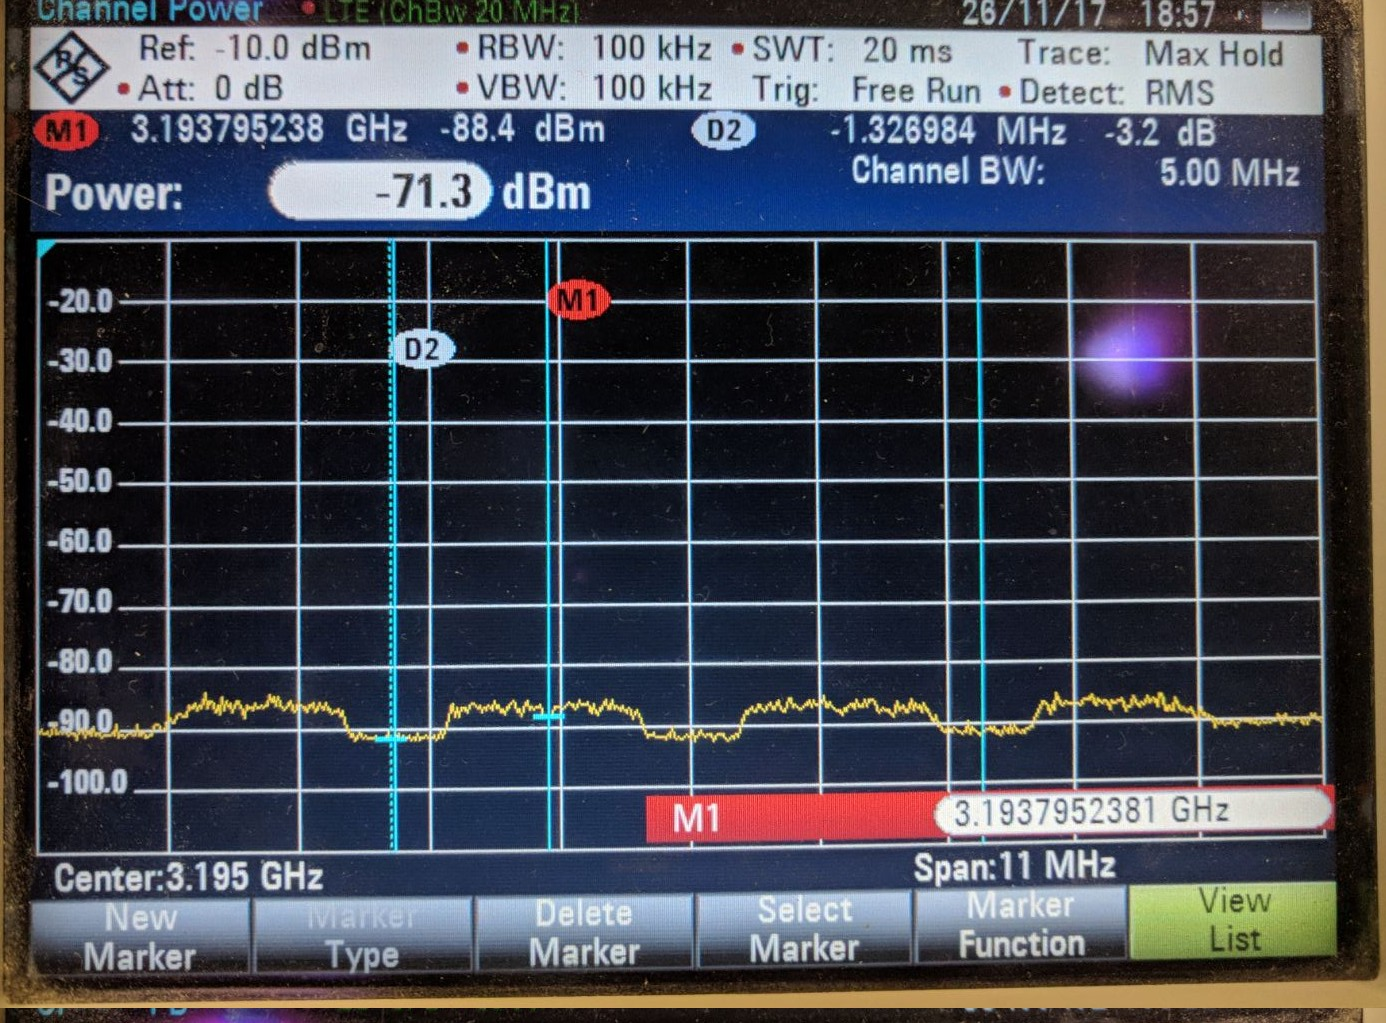
\includegraphics[width=\linewidth]{figures/snr_spec_5}
    \end{subfigure}
    \begin{subfigure}[htb]{0.45\textwidth}
        \centering
        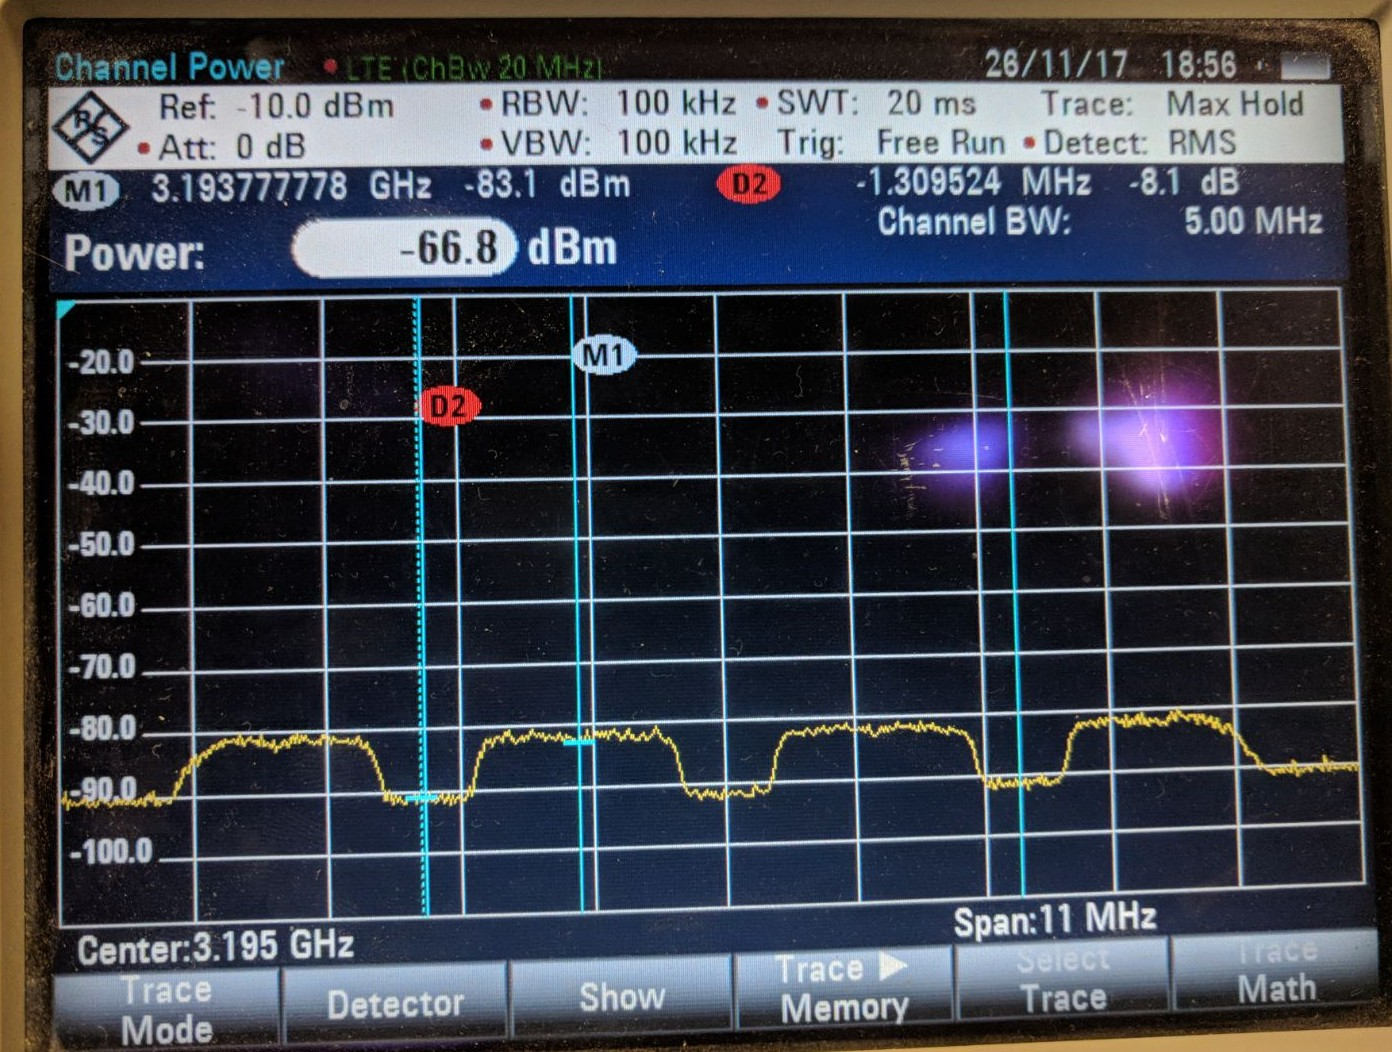
\includegraphics[width=\linewidth]{figures/snr_spec_10}
    \end{subfigure}
    \caption{Calibration of gain variation on PU transmitter (5dB variation)}
    \label{fig:snr_spec}
\end{figure}

\begin{figure}[!htb]
    \centering
    \begin{subfigure}[htb]{0.45\textwidth}
        \centering
        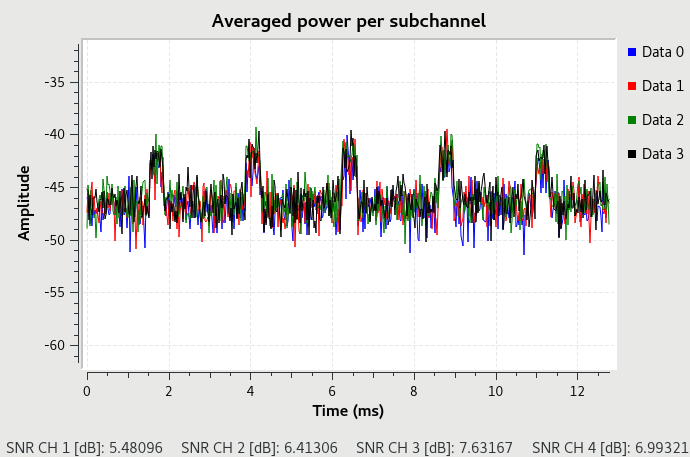
\includegraphics[width=\linewidth]{figures/snr_receiv_5}
        \caption{SNR={\raise.17ex\hbox{$\scriptstyle\sim$}}5dB}
    \end{subfigure}
    \begin{subfigure}[htb]{0.45\textwidth}
        \centering
        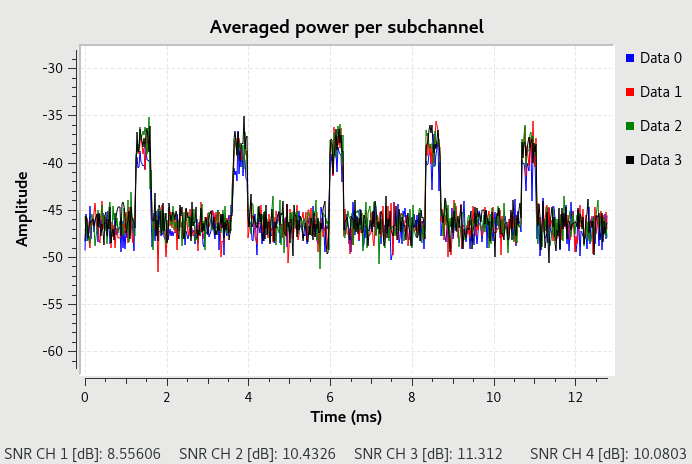
\includegraphics[width=\linewidth]{figures/snr_receiv_10}
        \caption{SNR={\raise.17ex\hbox{$\scriptstyle\sim$}}10dB}
    \end{subfigure}
    \caption{SNR display at receive side}
    \label{fig:snr_receiv}
\end{figure}

\subsection{Feature Engineering}\label{ch:features}
Having recorded the raw I/Q samples, it is required to apply signal processing techniques in order to extract features that this data could contain and that would be representative to identify the scenario that the \ac{PU} transmission is describing. For this, the implementation that was used in \cite{Wunsch2017} was used. The flowgraph that serves the purpose of feature extraction is shown in the Fig~\ref{fig:feature_extraction}. In Fig~\ref{fig:ed}, the files recorded from the \ac{PU} transmission are passed through an \ac{FFT}, and then the "Energy Detection" block is in charge of determining which channel has a measure of energy greater than the given threshold, which can be set as a block parameter. This block has 8 outputs: the top four provide the average power per subchannel, useful for plotting. Fig.~\ref{fig:snr_receiv} was plotted using these outputs. The bottom four send simply ones when the channel is identified as occupied, and zeros if the channel is identified as free.

\begin{figure}[!htb]
    \centering
    \begin{subfigure}[htb]{\textwidth}
        \centering
        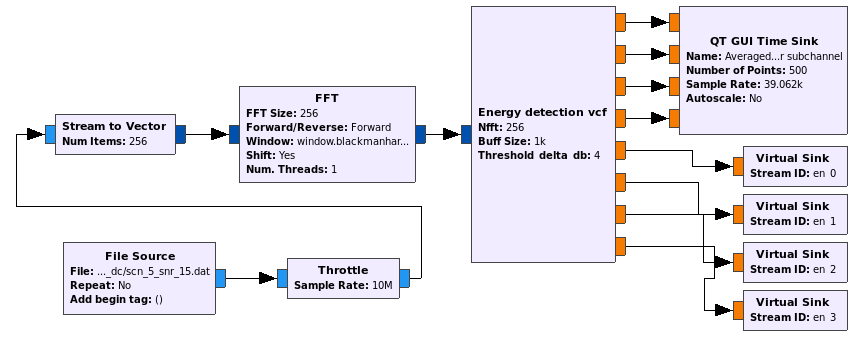
\includegraphics[width=\linewidth]{figures/feature_extraction_1}
        \caption{Energy Detection}
        \label{fig:ed}
    \end{subfigure}
    \begin{subfigure}[htb]{\textwidth}
        \centering
        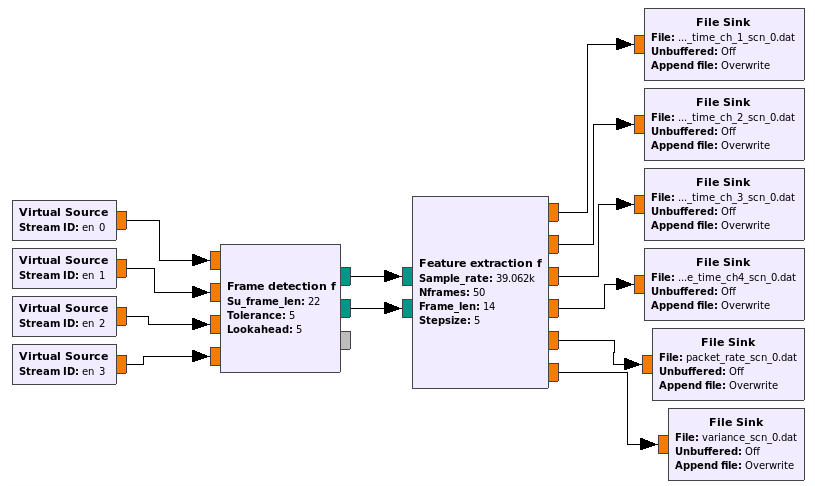
\includegraphics[width=\linewidth]{figures/feature_extraction_2}
        \caption{Frame Events detection and write features to file}
        \label{fig:frame_events}
    \end{subfigure}
    \caption{GNU Radio Flowgraph for feature extraction}
    \label{fig:feature_extraction}
\end{figure}

The second part of the flowgraph, shown in Fig~\ref{fig:frame_events} uses the boolean-like output from the "energy detection" block and analyzes them as \emph{frame events}, identifying the frames over the air and categorizing them as \ac{PU} frames or \ac{SU} frames based on its length, and generating these frame events if the analyzed frame per channel corresponds to the \ac{PU}.  Then, these events are taken to the "Feature Extraction" block, which generates three main features based on its inputs:

\begin{itemize}
    \item the average interframe time, i.e. the time delay between \ac{PU} frames.
    \item the packet rate, meaning the number of packets/frames that are passing through per second.
    \item the variance of the interframe time, which intends to determine if this interframe time is deterministic or stochastic and, if the later, with which variation.
\end{itemize}

Although these are effectively only three features, the interframe time is analyzed per channel, which explains the 6 outputs of the "feature extraction" block. This information is then written to disk in different files. This procedure is repeated for all the files saved during the process described in section ~\ref{ch:measure}, generating a total of:

\begin{equation}
    \text{10 scenarios} \cdot \text{ 7 SNR levels } \cdot \text{6 feature files } = \text{ 420 files }
\end{equation}

These files are provided in the final dataset product of this work, and a convenient script that automates the process of the feature extraction is provided at \cite{repo:cognitive_radio_ml}. As stated at the beginning of the chapter, these features are used for supervised learning, and the results are recorded in chapter~\ref{ch:evaluation}

\subsection{Spectrogram generation}\label{ch:spectrogram}

The feature extraction process is convenient and works well as seen in \cite{Wunsch2017}. However, it depends on a good \ac{PU} power level in order for the frame events to be generated. A way to go about this limitation is applying a different technology, such as image recognition using \ac{ConvNet}. The idea is to generate images that describe the unique characteristics of each scenario, and feed them to an image classificator. The images that better suit this need are the spectrograms. Based on the work of \cite{Paisana2017}, spectrograms were generated using the GNU Radio flowgraph shown in Fig~\ref{fig:specgram_generation}

\begin{figure}[!htb]
    \centering
    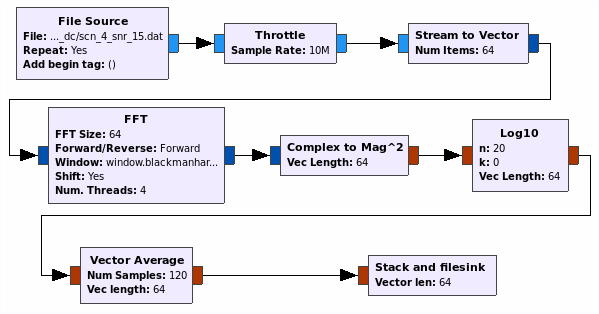
\includegraphics[width=\textwidth]{figures/specgram_generation}
    \caption{GNU Radio Flowgraph for spectrogram generation}
    \label{fig:specgram_generation}
\end{figure}

Most of the procedure is rather straightforward: the I/Q data files are read and the signal stream is fed into a vector for the \ac{FFT} calculation. The target images have a 64x64 pixels dimension, so that sets as well the FFT size to 64, and the blocks that follow calculate the power of the signal in dB. The last two blocks require a more detailed explanation.
The "Vector average" block calculates the arithmetic mean over a certain amount of vectors, as seen in Fig~\ref{fig:vectoravg}. For the sake of clarity, it can be assumed that this block operates on a matrix (or a 2-dimensional array) of dimensions NxM, being M the length of the input vectors, set in the block via the parameter "vector length" and set to 64 in this specific case, and N the number of vectors to operate, set in the block via the parameter "Num Samples" and set to 120. \\

\begin{figure}[!htb]
    \centering
    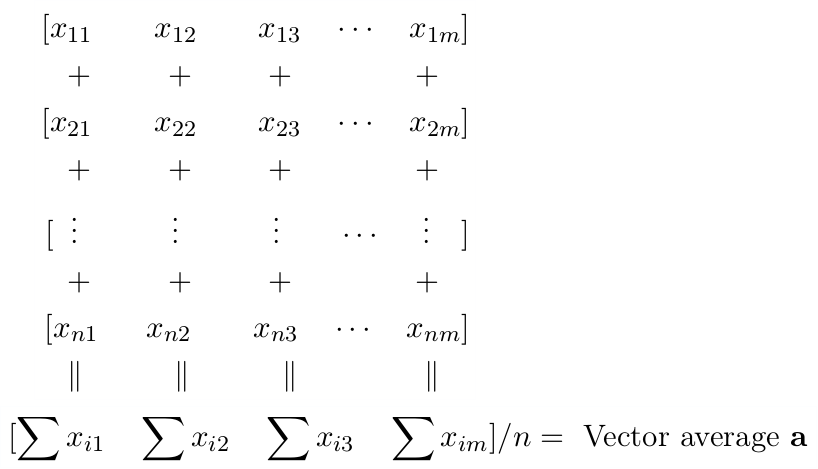
\includegraphics[width=0.7\textwidth]{figures/vectoravg}
    \caption{Operations made in "Vector Average" block}
    \label{fig:vectoravg}
\end{figure}

%\begin{align*}
    %[x_{11}\quad \quad x_{12} \quad \quad x_{13}\quad \cdots\quad x_{1m}] \\
       %+   \qquad \;  + \qquad \; +  \quad \quad \quad \quad + \quad     \\
    %[x_{21}\quad \quad x_{22} \quad \quad x_{23}\quad \cdots\quad x_{2m}] \\
       %+   \qquad \;  + \qquad \; +  \quad \quad \quad \quad + \quad     \\
    %[\; \; \vdots \qquad \quad \vdots \qquad \quad \vdots \quad  \; \; \; \cdots \quad \; \vdots \quad] \\
       %+   \qquad \;  + \qquad \; +  \quad \quad \quad \quad + \quad     \\
    %[x_{n1} \quad \; \; x_{n2} \qquad x_{n3}\quad \cdots\quad x_{nm}] \\
    %\; \; \; \parallel \qquad \quad \parallel \qquad \quad \parallel \quad  \; \; \;  \qquad \; \parallel \quad \\
%\end{align*}
%\[
    %[\sum{x_{i1}} \quad \sum{x_{i2}} \quad \sum{x_{i3}} \quad \sum{x_{im}}] / n = \text{ Vector average }\mathbf{a}
%\]
%\[
%\begin{bmatrix}
    %a_{11} & a_{12} & a_{13} & \dots  & a_{1m} \\
    %a_{21} & a_{22} & a_{23} & \dots  & a_{2m} \\
    %\vdots & \vdots & \vdots & \ddots & \vdots \\
    %a_{m1} & a_{m2} & a_{m3} & \dots  & a_{mm}
%\end{bmatrix}
%\]
%\begin{align*}
    %[a_{11}\quad \quad a_{12} \quad \quad a_{13}\quad \cdots\quad a_{1m}] \\
    %[a_{21}\quad \quad a_{22} \quad \quad a_{23}\quad \cdots\quad a_{2m}] \\
    %[\; \; \vdots \qquad \;\;\; \vdots \qquad \quad \vdots \quad  \; \; \; \cdots \quad \; \vdots \quad] \\
    %[a_{m1} \; \quad a_{m2} \qquad a_{m3} \;\;\;  \cdots \;\; a_{mm}] \\
%\end{align*}

\begin{figure}[!htb]
    \centering
    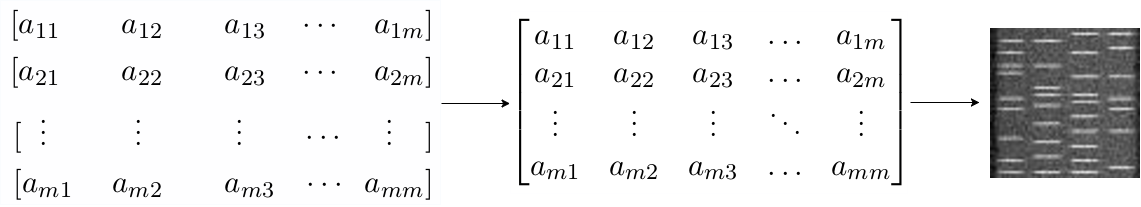
\includegraphics[width=\textwidth]{figures/stack_n_save}
    \caption{Operations made in "Stack and File sink" block}
    \label{fig:stacknsave}
\end{figure}

The block takes 120 vectors and presents at its output the arithmetic mean according to the matrix. After that, the block "Stack and file sink" takes 64 averaged vectors, stacks them vertically and generates an image object that is later saved as a JPEG image to disk, as seen in Fig~\ref{fig:stacknsave}. Given the sample rate of the system set to 10Msps, this means that each spectrogram image will contain the information equivalent to 0.768 x 64 = 49.2ms of data. These images are then used for the image classification. From the files recorded using the procedure described in section~\ref{ch:measure}, a total of 84700 pictures is generated, from which 90\% is used for training the \ac{ConvNet} and 10\% is used as testing set.


  \acresetall
\chapter{Evaluation and Results}\label{ch:evaluation}
In this chapter, a benchmark of the analyzed algorithms is presented, based on dataset size and complexity. For the first part, the algorithms used for supervised learning are presented, for which an analysis of the different complexities used is made. From the benchmark, the trained models with the best performance are saved and then used in the live implementation presented in chapter~\ref{ch:live}. The process of saving trained models for later use is called \emph{model persistence}.

\section{Performance metrics}\label{ch:performance}

The impact of the dataset size on the algorithm performance is of special interest. Given that the data recorded using the procedure described in section~\ref{ch:measure} has a fixed size, this analysis was performed by slicing the resulting feature extraction files to emulate different dataset sizes. It is important to notice that only "slicing", in order to emulate smaller datasets, and not "repeating samples", for emulation of bigger datasets, has a significant impact on the performance, as noted in section~\ref{ch:size}. This is due to the fact that repeated samples present no new information to the model, and there is nothing new to learn from them.

The dataset is, then, sliced into four different sizes:

\begin{itemize}
    \item Small dataset (S): is one fourth (1/4) of the original dataset
    \item Medium dataset (M): is one third (1/3) of the original dataset
    \item Large dataset (L): is half (1/2) of the original dataset
    \item Extra Large dataset (XL): the whole set of features extracted as recorded from the signals over the air.
\end{itemize}

Furthermore, a benchmark of the learning algorithms is made based on variations on their complexities. Each algorithm has different ways to represent its own complexity, and this has a significant impact on its overall performance. The \ac{ML} algorithms used in this analysis are K-nearest neighbors, \ac{SVM} and binary tree classification. Their complexities are set as follows:

\begin{itemize}
    \item K-nearest neighbors: the complexity of this algorithm is set by the amount of neighbors that are considered in order to make a classification decision. For the benchmark, different models were trained using from 1 neighbor up to 200 neighbors
    \item \ac{SVM}: this algorithm allows the designer to select the type of kernel that is used during the learning process. The function of the kernel is to generate internally non-linear transformations over the input data while still behaving as a linear classificator. For this work, the \ac{RBF} is used as a kernel because of its known good performance on multiclass classification problems at the cost of longer training times. The complexity of this model is then set by providing different values to the '\(\gamma\)' parameter of this \ac{RBF} kernel, whose kernel function is:
        \begin{equation}
            \text{exp}(-\gamma || x - x'||^2
        \end{equation}
        For this work, values of \(\gamma=2^{-15}, 2^{-13}, 2^{-11}, 2^{-9}, 2^{-7}, 2^{-5}, 2^{-3}, 2^{-1}, 2^{1} \text{ and }2^{3} \) are used.


    \item Decision Trees: in this model, the complexity is ruled by the depth of the decision branch. Here, depths from 1 up to 500 are used.
\end{itemize}

Moreover, it is also interesting to determine how the models behave when the features have been scaled. A first glance at the impact of a scaler is presented by using the StandardScaler() from SKlearn, which simply removes the mean of the features and scales them to unit variance. A side-by-side comparison of model performance when trained with unscaled features vs.scaled features is shown as a result of the benchmark. The results are depicted in Figs~\ref{fig:knn}, \ref{fig:dtc} and \ref{fig:svc}.

\begin{figure}[!htb]
    \centering
    \begin{subfigure}[t]{0.49\textwidth}
        \centering
        \begin{tikzpicture}[scale=0.8]
            \begin{axis}[
                xlabel={\# of Neighbors},
                ylabel={Accuracy},
                legend style={at={(1.2,1.20)},
                    anchor=north,legend columns=-1},
                  ]
                \addplot[color=blue] table [x=N, y=S, col sep=comma, mark=none] {data/knn_accs.csv};
                \addplot[color=red] table [x=N, y=M, col sep=comma, mark=none] {data/knn_accs.csv};
                \addplot[color=green] table [x=N, y=L, col sep=comma, mark=none] {data/knn_accs.csv};
                \addplot[color=orange] table [x=N, y=XL, col sep=comma, mark=none] {data/knn_accs.csv};
                \legend{Dataset S, Dataset M, Dataset L, Dataset XL}
        \end{axis}
        \end{tikzpicture}
        \caption{Accuracy with unscaled features}
        \label{fig:knn_accs_scaled}
    \end{subfigure}
        \hfill
    \begin{subfigure}[t]{0.49\textwidth}
        \centering
        \begin{tikzpicture}[scale=0.8]
            \begin{axis}[
                xlabel={\# of Neighbors},
                ylabel={Accuracy},
                  ]
                \addplot[color=blue] table [x=N, y=S, col sep=comma, mark=none] {data/knn_accs_scaled.csv};
                \addplot[color=red] table [x=N, y=M, col sep=comma, mark=none] {data/knn_accs_scaled.csv};
                \addplot[color=green] table [x=N, y=L, col sep=comma, mark=none] {data/knn_accs_scaled.csv};
                \addplot[color=orange] table [x=N, y=XL, col sep=comma, mark=none] {data/knn_accs_scaled.csv};
        \end{axis}
        \end{tikzpicture}
        \caption{Accuracy with scaled features}
        \label{fig:knn_accs_scaled}
    \end{subfigure}
    \begin{subfigure}[t]{0.49\textwidth}
        \centering
        \begin{tikzpicture}[scale=0.8]
            \begin{axis}[
                xlabel={\# of Neighbors},
                ylabel={Training time (s)},
                  ]
                \addplot[color=blue]table [x=N, y=S, col sep=comma, mark=none] {data/knn_fit_times.csv};
                \addplot[color=red] table [x=N, y=M, col sep=comma, mark=none] {data/knn_fit_times.csv};
                \addplot[color=green] table [x=N, y=L, col sep=comma, mark=none] {data/knn_fit_times.csv};
                \addplot[color=orange] table [x=N, y=XL, col sep=comma, mark=none] {data/knn_fit_times.csv};
        \end{axis}
        \end{tikzpicture}
        \caption{Training times with unscaled features}
        \label{fig:knn_fit_times}
    \end{subfigure}
    \centering
        \hfill
    \begin{subfigure}[t]{0.49\textwidth}
        \centering
        \begin{tikzpicture}[scale=0.8]
            \begin{axis}[
                xlabel={\# of Neighbors},
                ylabel={Training time (s)},
                  ]
                \addplot[color=blue]table [x=N, y=S, col sep=comma, mark=none] {data/knn_fit_times_scaled.csv};
                \addplot[color=red] table [x=N, y=M, col sep=comma, mark=none] {data/knn_fit_times_scaled.csv};
                \addplot[color=green] table [x=N, y=L, col sep=comma, mark=none] {data/knn_fit_times_scaled.csv};
                \addplot[color=orange] table [x=N, y=XL, col sep=comma, mark=none] {data/knn_fit_times_scaled.csv};
        \end{axis}
        \end{tikzpicture}
        \caption{Training times with scaled features}
        \label{fig:knn_fit_times_scaled}
    \end{subfigure}
    \begin{subfigure}[t]{0.49\textwidth}
        \centering
        \begin{tikzpicture}[scale=0.8]
            \begin{axis}[
                xlabel={\# of Neighbors},
                ylabel={Prediction time (s)},
                  ]
                \addplot[color=blue]table [x=N, y=S, col sep=comma, mark=none] {data/knn_pred_times.csv};
                \addplot[color=red] table [x=N, y=M, col sep=comma, mark=none] {data/knn_pred_times.csv};
                \addplot[color=green] table [x=N, y=L, col sep=comma, mark=none] {data/knn_pred_times.csv};
                \addplot[color=orange] table [x=N, y=XL, col sep=comma, mark=none] {data/knn_pred_times.csv};
        \end{axis}
        \end{tikzpicture}
        \caption{Prediction times with unscaled features}
        \label{fig:knn_pred_times}
    \end{subfigure}
    \centering
        \hfill
    \begin{subfigure}[t]{0.49\textwidth}
        \centering
        \begin{tikzpicture}[scale=0.8]
            \begin{axis}[
                xlabel={\# of Neighbors},
                ylabel={Prediction time (s)},
                  ]
                \addplot[color=blue]table [x=N, y=S, col sep=comma, mark=none] {data/knn_pred_times_scaled.csv};
                \addplot[color=red] table [x=N, y=M, col sep=comma, mark=none] {data/knn_pred_times_scaled.csv};
                \addplot[color=green] table [x=N, y=L, col sep=comma, mark=none] {data/knn_pred_times_scaled.csv};
                \addplot[color=orange] table [x=N, y=XL, col sep=comma, mark=none] {data/knn_pred_times_scaled.csv};
        \end{axis}
        \end{tikzpicture}
        \caption{Prediction times with scaled features}
        \label{fig:knn_pred_times}
    \end{subfigure}
    \caption{Metrics for K-Nearest Neighbors}
    \label{fig:knn}
\end{figure}

\begin{figure}[!htb]
    \centering
    \begin{subfigure}[t]{0.49\textwidth}
        \centering
        \begin{tikzpicture}[scale=0.8]
            \begin{axis}[
                xlabel={Tree depth},
                ylabel={Accuracy},
                legend style={at={(1.2,1.20)},
                    anchor=north,legend columns=-1},
                  ]
                \addplot[color=blue] table [x=N, y=S, col sep=comma, mark=none] {data/dtc_accs.csv};
                \addplot[color=red] table [x=N, y=M, col sep=comma, mark=none] {data/dtc_accs.csv};
                \addplot[color=green] table [x=N, y=L, col sep=comma, mark=none] {data/dtc_accs.csv};
                \addplot[color=orange] table [x=N, y=XL, col sep=comma, mark=none] {data/dtc_accs.csv};
                \legend{Dataset S, Dataset M, Dataset L, Dataset XL}
        \end{axis}
        \end{tikzpicture}
        \caption{Accuracy with unscaled features}
        \label{fig:dtc_accs_scaled}
    \end{subfigure}
        \hfill
    \begin{subfigure}[t]{0.49\textwidth}
        \centering
        \begin{tikzpicture}[scale=0.8]
            \begin{axis}[
                xlabel={Tree depth},
                ylabel={Accuracy},
                  ]
                \addplot[color=blue] table [x=N, y=S, col sep=comma, mark=none] {data/dtc_accs_scaled.csv};
                \addplot[color=red] table [x=N, y=M, col sep=comma, mark=none] {data/dtc_accs_scaled.csv};
                \addplot[color=green] table [x=N, y=L, col sep=comma, mark=none] {data/dtc_accs_scaled.csv};
                \addplot[color=orange] table [x=N, y=XL, col sep=comma, mark=none] {data/dtc_accs_scaled.csv};
        \end{axis}
        \end{tikzpicture}
        \caption{Accuracy with scaled features}
        \label{fig:dtc_accs_scaled}
    \end{subfigure}
    \begin{subfigure}[t]{0.49\textwidth}
        \centering
        \begin{tikzpicture}[scale=0.8]
            \begin{axis}[
                xlabel={Tree depth},
                ylabel={Training time (s)},
                  ]
                \addplot[color=blue]table [x=N, y=S, col sep=comma, mark=none] {data/dtc_fit_times.csv};
                \addplot[color=red] table [x=N, y=M, col sep=comma, mark=none] {data/dtc_fit_times.csv};
                \addplot[color=green] table [x=N, y=L, col sep=comma, mark=none] {data/dtc_fit_times.csv};
                \addplot[color=orange] table [x=N, y=XL, col sep=comma, mark=none] {data/dtc_fit_times.csv};
        \end{axis}
        \end{tikzpicture}
        \caption{Training times with unscaled features}
        \label{fig:dtc_fit_times}
    \end{subfigure}
    \centering
        \hfill
    \begin{subfigure}[t]{0.49\textwidth}
        \centering
        \begin{tikzpicture}[scale=0.8]
            \begin{axis}[
                xlabel={Tree depth},
                ylabel={Training time (s)},
                  ]
                \addplot[color=blue]table [x=N, y=S, col sep=comma, mark=none] {data/dtc_fit_times_scaled.csv};
                \addplot[color=red] table [x=N, y=M, col sep=comma, mark=none] {data/dtc_fit_times_scaled.csv};
                \addplot[color=green] table [x=N, y=L, col sep=comma, mark=none] {data/dtc_fit_times_scaled.csv};
                \addplot[color=orange] table [x=N, y=XL, col sep=comma, mark=none] {data/dtc_fit_times_scaled.csv};
        \end{axis}
        \end{tikzpicture}
        \caption{Training times with scaled features}
        \label{fig:dtc_fit_times_scaled}
    \end{subfigure}
    \begin{subfigure}[t]{0.49\textwidth}
        \centering
        \begin{tikzpicture}[scale=0.8]
            \begin{axis}[
                xlabel={Tree depth},
                ylabel={Prediction time (s)},
                  ]
                \addplot[color=blue]table [x=N, y=S, col sep=comma, mark=none] {data/dtc_pred_times.csv};
                \addplot[color=red] table [x=N, y=M, col sep=comma, mark=none] {data/dtc_pred_times.csv};
                \addplot[color=green] table [x=N, y=L, col sep=comma, mark=none] {data/dtc_pred_times.csv};
                \addplot[color=orange] table [x=N, y=XL, col sep=comma, mark=none] {data/dtc_pred_times.csv};
        \end{axis}
        \end{tikzpicture}
        \caption{Prediction times with unscaled features}
        \label{fig:dtc_pred_times}
    \end{subfigure}
    \centering
        \hfill
    \begin{subfigure}[t]{0.49\textwidth}
        \centering
        \begin{tikzpicture}[scale=0.8]
            \begin{axis}[
                xlabel={Tree depth},
                ylabel={Prediction time (s)},
                  ]
                \addplot[color=blue]table [x=N, y=S, col sep=comma, mark=none] {data/dtc_pred_times_scaled.csv};
                \addplot[color=red] table [x=N, y=M, col sep=comma, mark=none] {data/dtc_pred_times_scaled.csv};
                \addplot[color=green] table [x=N, y=L, col sep=comma, mark=none] {data/dtc_pred_times_scaled.csv};
                \addplot[color=orange] table [x=N, y=XL, col sep=comma, mark=none] {data/dtc_pred_times_scaled.csv};
        \end{axis}
        \end{tikzpicture}
        \caption{Prediction times with scaled features}
        \label{fig:dtc_pred_times}
    \end{subfigure}
    \caption{Metrics for the decision tree classifier}
    \label{fig:dtc}
\end{figure}



\begin{figure}[!htb]
    \centering
    \begin{subfigure}[t]{0.49\textwidth}
        \centering
        \begin{tikzpicture}[scale=0.8]
            \begin{axis}[
                    xlabel={\(\gamma\) for \ac{RBF} kernel - \ac{SVM}},
                ylabel={Accuracy},
                legend style={at={(1.2,1.20)},
                    anchor=north,legend columns=-1},
                  ]
                \addplot[color=blue] table [x=N, y=S, col sep=comma, mark=none] {data/svc_accs.csv};
                \addplot[color=red] table [x=N, y=M, col sep=comma, mark=none] {data/svc_accs.csv};
                \addplot[color=green] table [x=N, y=L, col sep=comma, mark=none] {data/svc_accs.csv};
                \addplot[color=orange] table [x=N, y=XL, col sep=comma, mark=none] {data/svc_accs.csv};
                \legend{Dataset S, Dataset M, Dataset L, Dataset XL}
        \end{axis}
        \end{tikzpicture}
        \caption{Accuracy with unscaled features}
        \label{fig:svc_accs_scaled}
    \end{subfigure}
        \hfill
    \begin{subfigure}[t]{0.49\textwidth}
        \centering
        \begin{tikzpicture}[scale=0.8]
            \begin{axis}[
                    xlabel={\(\gamma\) for \ac{RBF} kernel - \ac{SVM}},
                ylabel={Accuracy},
                  ]
                \addplot[color=blue] table [x=N, y=S, col sep=comma, mark=none] {data/svc_accs_scaled.csv};
                \addplot[color=red] table [x=N, y=M, col sep=comma, mark=none] {data/svc_accs_scaled.csv};
                \addplot[color=green] table [x=N, y=L, col sep=comma, mark=none] {data/svc_accs_scaled.csv};
                \addplot[color=orange] table [x=N, y=XL, col sep=comma, mark=none] {data/svc_accs_scaled.csv};
        \end{axis}
        \end{tikzpicture}
        \caption{Accuracy with scaled features}
        \label{fig:svc_accs_scaled}
    \end{subfigure}
    \begin{subfigure}[t]{0.49\textwidth}
        \centering
        \begin{tikzpicture}[scale=0.8]
            \begin{axis}[
                    xlabel={\(\gamma\) for \ac{RBF} kernel - \ac{SVM}},
                ylabel={Training time (s)},
                  ]
                \addplot[color=blue]table [x=N, y=S, col sep=comma, mark=none] {data/svc_fit_times.csv};
                \addplot[color=red] table [x=N, y=M, col sep=comma, mark=none] {data/svc_fit_times.csv};
                \addplot[color=green] table [x=N, y=L, col sep=comma, mark=none] {data/svc_fit_times.csv};
                \addplot[color=orange] table [x=N, y=XL, col sep=comma, mark=none] {data/svc_fit_times.csv};
        \end{axis}
        \end{tikzpicture}
        \caption{Training times with unscaled features}
        \label{fig:svc_fit_times}
    \end{subfigure}
    \centering
        \hfill
    \begin{subfigure}[t]{0.49\textwidth}
        \centering
        \begin{tikzpicture}[scale=0.8]
            \begin{axis}[
                    xlabel={\(\gamma\) for \ac{RBF} kernel - \ac{SVM}},
                ylabel={Training time (s)},
                  ]
                \addplot[color=blue]table [x=N, y=S, col sep=comma, mark=none] {data/svc_fit_times_scaled.csv};
                \addplot[color=red] table [x=N, y=M, col sep=comma, mark=none] {data/svc_fit_times_scaled.csv};
                \addplot[color=green] table [x=N, y=L, col sep=comma, mark=none] {data/svc_fit_times_scaled.csv};
                \addplot[color=orange] table [x=N, y=XL, col sep=comma, mark=none] {data/svc_fit_times_scaled.csv};
        \end{axis}
        \end{tikzpicture}
        \caption{Training times with scaled features}
        \label{fig:svc_fit_times_scaled}
    \end{subfigure}
    \begin{subfigure}[t]{0.49\textwidth}
        \centering
        \begin{tikzpicture}[scale=0.8]
            \begin{axis}[
                    xlabel={\(\gamma\) for \ac{RBF} kernel - \ac{SVM}},
                ylabel={Prediction time (s)},
                  ]
                \addplot[color=blue]table [x=N, y=S, col sep=comma, mark=none] {data/svc_pred_times.csv};
                \addplot[color=red] table [x=N, y=M, col sep=comma, mark=none] {data/svc_pred_times.csv};
                \addplot[color=green] table [x=N, y=L, col sep=comma, mark=none] {data/svc_pred_times.csv};
                \addplot[color=orange] table [x=N, y=XL, col sep=comma, mark=none] {data/svc_pred_times.csv};
        \end{axis}
        \end{tikzpicture}
        \caption{Prediction times with unscaled features}
        \label{fig:svc_pred_times}
    \end{subfigure}
    \centering
        \hfill
    \begin{subfigure}[t]{0.49\textwidth}
        \centering
        \begin{tikzpicture}[scale=0.8]
            \begin{axis}[
                    xlabel={\(\gamma\) for \ac{RBF} kernel - \ac{SVM}},
                ylabel={Prediction time (s)},
                  ]
                \addplot[color=blue]table [x=N, y=S, col sep=comma, mark=none] {data/svc_pred_times_scaled.csv};
                \addplot[color=red] table [x=N, y=M, col sep=comma, mark=none] {data/svc_pred_times_scaled.csv};
                \addplot[color=green] table [x=N, y=L, col sep=comma, mark=none] {data/svc_pred_times_scaled.csv};
                \addplot[color=orange] table [x=N, y=XL, col sep=comma, mark=none] {data/svc_pred_times_scaled.csv};
        \end{axis}
        \end{tikzpicture}
        \caption{Prediction times with scaled features}
        \label{fig:svc_pred_times}
    \end{subfigure}
    \caption{Metrics for \ac{SVM}}
    \label{fig:svc}
\end{figure}




%\begin{figure}[!htb]
    %\centering
    %\begin{subfigure}[htb]{0.49\textwidth}
        %\centering
        %\includestandalone[width=\linewidth]{figures/knn_accs}
        %\label{fig:knn_accs}
    %\end{subfigure}
    %\begin{subfigure}[htb]{0.49\textwidth}
        %\centering
        %\includestandalone[width=\linewidth]{figures/knn_accs_scaled}
        %\caption{Accuracy with scaled features}
        %\label{fig:knn_accs_scaled}
    %\end{subfigure}\\
    %\begin{subfigure}[htb]{0.49\textwidth}
        %\centering
        %\includestandalone[width=\linewidth]{figures/knn_fit_times}
        %\caption{Training times with unscaled features}
        %\label{fig:knn_fit_times}
    %\end{subfigure}
    %\begin{subfigure}[htb]{0.49\textwidth}
        %\centering
        %\includestandalone[width=\linewidth]{figures/knn_fit_times_scaled}
        %\caption{Training times with scaled features}
        %\label{fig:knn_fit_times_scaled}
    %\end{subfigure}\\
    %\begin{subfigure}[htb]{0.49\textwidth}
        %\centering
        %\includestandalone[width=\linewidth]{figures/knn_pred_times}
        %\caption{Prediction times with unscaled features}
        %\label{fig:knn_pred_times}
    %\end{subfigure}
    %\begin{subfigure}[htb]{0.49\textwidth}
        %\centering
        %\includestandalone[width=\linewidth]{figures/knn_pred_times_scaled}
        %\caption{Prediction times with scaled features}
        %\label{fig:knn_pred_times_scaled}
    %\end{subfigure}
    %\caption{K-nearest Neighbors}
    %\label{fig:knn}
%\end{figure}

%\begin{figure}[!htb]
    %\centering
    %\begin{subfigure}[htb]{0.49\textwidth}
        %\centering
        %\includestandalone[width=\linewidth]{figures/dtc_accs}
        %\caption{Accuracy with unscaled features}
        %\label{fig:dtc_accs}
    %\end{subfigure}
    %\begin{subfigure}[htb]{0.49\textwidth}
        %\centering
        %\includestandalone[width=\linewidth]{figures/dtc_accs_scaled}
        %\caption{Accuracy with scaled features}
        %\label{fig:dtc_accs_scaled}
    %\end{subfigure}
    %\begin{subfigure}[htb]{0.49\textwidth}
        %\centering
        %\includestandalone[width=\linewidth]{figures/dtc_fit_times}
        %\caption{Training times with unscaled features}
        %\label{fig:dtc_fit_times}
    %\end{subfigure}
    %\begin{subfigure}[htb]{0.49\textwidth}
        %\centering
        %\includestandalone[width=\linewidth]{figures/dtc_fit_times_scaled}
        %\caption{Training times with scaled features}
        %\label{fig:dtc_fit_times_scaled}
    %\end{subfigure}
    %\begin{subfigure}[htb]{0.49\textwidth}
        %\centering
        %\includestandalone[width=\linewidth]{figures/dtc_pred_times}
        %\caption{Prediction times with unscaled features}
        %\label{fig:dtc_pred_times}
    %\end{subfigure}
    %\begin{subfigure}[htb]{0.49\textwidth}
        %\centering
        %\includestandalone[width=\linewidth]{figures/dtc_pred_times_scaled}
        %\caption{Prediction times with scaled features}
        %\label{fig:dtc_pred_times_scaled}
    %\end{subfigure}
    %\caption{Decision Trees}
    %\label{fig:dtc}
%\end{figure}

%\begin{figure}
    %\centering
    %\begin{subfigure}[htb]{0.49\textwidth}
        %\centering
        %\includestandalone[width=\linewidth]{figures/svc_accs}
        %\caption{Accuracy with unscaled features}
        %\label{fig:svc_accs}
    %\end{subfigure}
    %\begin{subfigure}[htb]{0.49\textwidth}
        %\centering
        %\includestandalone[width=\linewidth]{figures/svc_accs_scaled}
        %\caption{Accuracy with scaled features}
        %\label{fig:svc_accs_scaled}
    %\end{subfigure}
    %\begin{subfigure}[b]{0.49\textwidth}
        %\centering
        %\includestandalone[width=\linewidth]{figures/svc_fit_times}
        %\caption{Training times with unscaled features}
        %\label{fig:svc_fit_times}
    %\end{subfigure}
    %\begin{subfigure}[b]{0.49\textwidth}
        %\centering
        %\includestandalone[width=\linewidth]{figures/svc_fit_times_scaled}
        %\caption{Training times with scaled features}
        %\label{fig:svc_fit_times_scaled}
    %\end{subfigure}
    %\begin{subfigure}[b]{0.49\textwidth}
        %\centering
        %\includestandalone[width=\linewidth]{figures/svc_pred_times}
        %\caption{Prediction times with unscaled features}
        %\label{fig:svc_pred_times}
    %\end{subfigure}
    %\begin{subfigure}[b]{0.49\textwidth}
        %\centering
        %\includestandalone[width=\linewidth]{figures/svc_pred_times_scaled}
        %\caption{Prediction times with scaled features}
        %\label{fig:dtc_pred_times_scaled}
    %\end{subfigure}
    %\caption{Support Vector Machines}
    %\label{fig:svc}
%\end{figure}

From Figs~\ref{fig:knn}, \ref{fig:dtc} and \ref{fig:svc} a couple of conclusions can be extracted. First, it is seen that the accuracy of the model increases as more data is taken into consideration, which is well according to the theory and serves as a catalyst for applying the same implementation with more data as proposed in chapter~\ref{ch:conclusions}. Furthermore, three different behaviors are appreciated:

\begin{itemize}
    \item As complexity increases, the K-nearest neighbors algorithm shows a decrease on its overall accuracy, which is an indication that the model is over-generalizing, and suggests that with such a complexity (above few neighbors), the model is starting to loosely classify scenarios, allowing more samples to be misclassified, and is set to perform badly if unknown samples are feed to it, as its capabilities for generalization are in decay. Moreover, the prediction times for the highest level of complexity are already about two times greater than the second highest, making high K-nearest neighbors complexity not suitable for live implementations. Furthermore, this model shows both a reduction in accuracy and an increase on prediction time when the features have been scaled, which simply states that the model performs well without further data preprocessing right after the feature extraction.
    \item The decision tree model shows a steady increase on its accuracy as complexity increases, without reaching a clear overfitting state. Complexity has a clear effect on the training times, but it is still in the range of the milliseconds - being a process done only once, this does not affect dramatically the model selection and does not close the possibility of increasing the complexity for this specific use case. This can also be backed by the fact that the prediction times seem to stay constant with this increase. Interestingly, not only the training times are reduced after scaling, but also the prediction times are drastically improved, reaching about 10x faster predictions using the standard scaler. With comparable accuracy, scaling the features seems like a prospect procedure when this model is used in time demanding or live implementations.
        The low accuracy of this model when a depth=2 does not come as a surprise. As the classification is done based on \emph{if-then} steps, having such a short depth can only provide four possible predicted values, as it can be seen in the extracted tree shown in Fig~\ref{fig:dt_2}. This model is generated as an experimental exercise to show this behavior, and to make the statement that the depth of the tree has to be able to generate at least as many answers as classes of the problem, which in this specific use case is achieved with a depth=\(2^4 > 10\). Graphical representations of complex decision trees are easily generated, but they become overwhelming for them to be shown in this print. The procedure to generate these trees is explained in the development notebook of this thesis \cite{repo:cognitive_radio_ml}.

\begin{figure}[!htb]
    \centering
      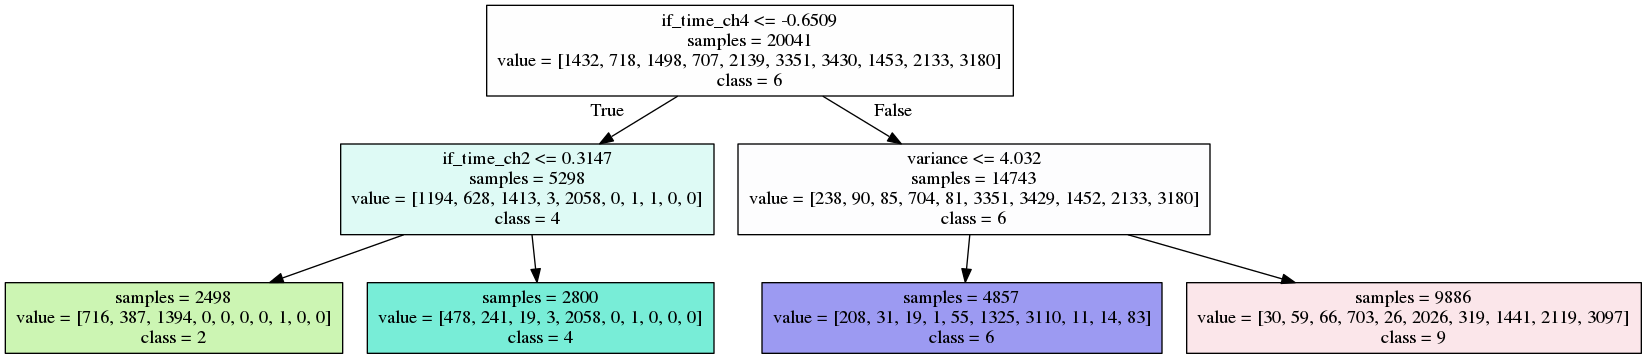
\includegraphics[width=\textwidth]{figures/dt_2}
      \caption{Extracted representation of a trained decision tree with depth=2}
      \label{fig:dt_2}
\end{figure}

    \item the \ac{SVM} show a clear tendency to improve as complexity is increased only if the data has been scaled, which indicates the sensitivity of this model to unscaled data.  However, the best accuracy of this model is still below the accuracies of the other models regarded in this benchmark. Additionally, the training and prediction times exceed dramatically the times achieved with the other models, being about 8000 times longer for training and around 500 times longer for prediction. The fact that this model is that slow will definitely affect considerably the performance of real-time implementations, an aspect that is crucial in systems such as cognitive radio, and therefore would not be recommended for that type of implementations.
\end{itemize}

\section{Scenario Classification}
Besides of the general performance that the learning models have in regard to the whole testing set, it is paramount to determine how good they perform by classifying each of the specific scenarios of Table~\ref{table:scenarios}. To assess this, confusion matrices are used to determine the number of correctly classified scenarios, along with the false positives and false negatives. On this analysis, it is only of interest the number of correctly classified scenarios, and any misclassification affects the implementation equally, regardless of its type. Moreover, in section~\ref{ch:performance} can be seen that each algorithm behaves differently in terms not only of accuracy, but also in training time and prediction time. As the models are trained only once, the "training time" does not play a role in the model selection for this work, as it does not have any repercussion on the performance of the model when new values are applied to it. Therefore, "prediction time" and "accuracy" are metrics of quality that are considered for these models on its selection to be applied on real-time scenarios.\\

Confusion matrices show how each of the samples from the data set are classified for a given model. As a matter of illustration, a side by side comparison for the worst-performing vs. the best-performing model, with respect to accuracy, is given in Fig~\ref{fig:confusionknn}, \ref{fig:confusiondtc} and \ref{fig:confusionsvc}. The complete set of confusion matrices, corresponding to every trained model, can be found in the development notebook for this work \cite{repo:cognitive_radio_ml}.


\begin{figure}[!htb]
    \captionsetup[subfigure]{justification=centering}
    \centering
    \begin{subfigure}[htb]{0.49\textwidth}
        \centering
        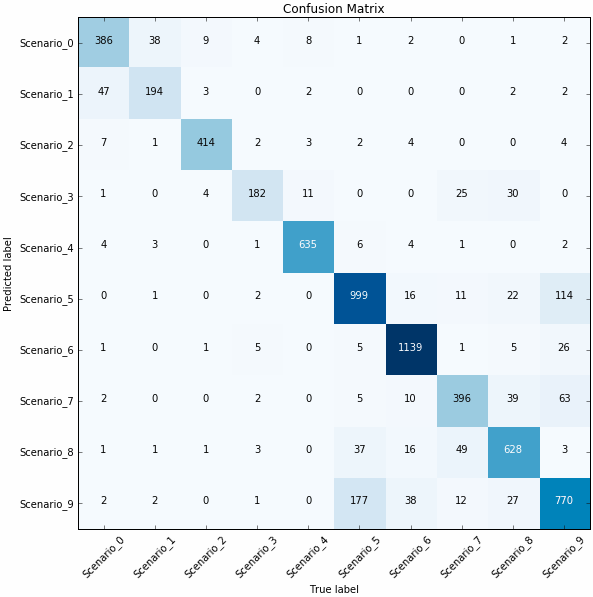
\includegraphics[width=\linewidth]{figures/knn_scaled_S_50}
        \caption{KNN-50 neighbors, StandardScaled, trained with small (S) dataset}
        \label{fig:knn_2}
    \end{subfigure}
    \begin{subfigure}[htb]{0.49\textwidth}
        \centering
        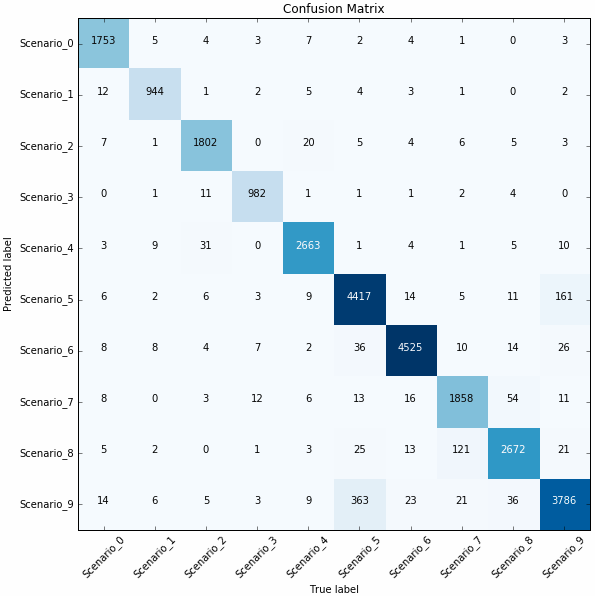
\includegraphics[width=\linewidth]{figures/knn_unscaled_XL_4}
        \caption{KNN-4 neighbors, unscaled, trained with whole (XL) dataset}
        \label{fig:knn_4}
    \end{subfigure}
    \caption{Confusion Matrixes for K-nearest Neighbor Models}
    \label{fig:confusionknn}
\end{figure}

\begin{figure}[!htb]
    \captionsetup[subfigure]{justification=centering}
    \centering
    \begin{subfigure}[htb]{0.49\textwidth}
        \centering
        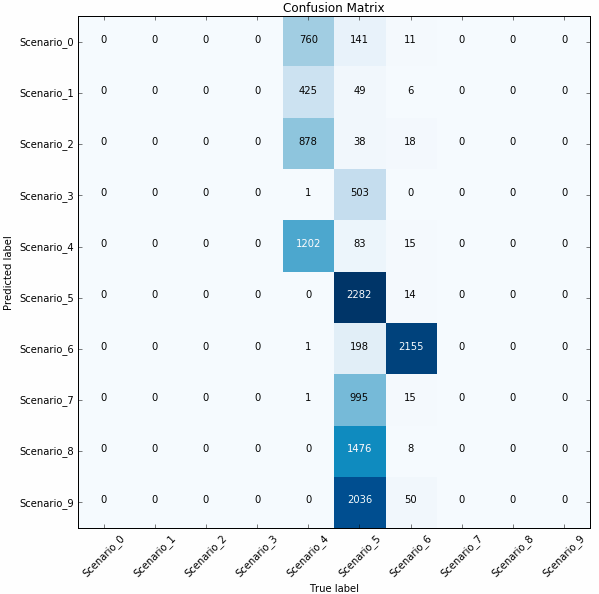
\includegraphics[width=\linewidth]{figures/dtc_unscaled_L_2}
        \caption{Decision Tree, unscaled, depth=2, trained with large (L) dataset}
        \label{fig:knn_2}
    \end{subfigure}
    \begin{subfigure}[htb]{0.49\textwidth}
        \centering
        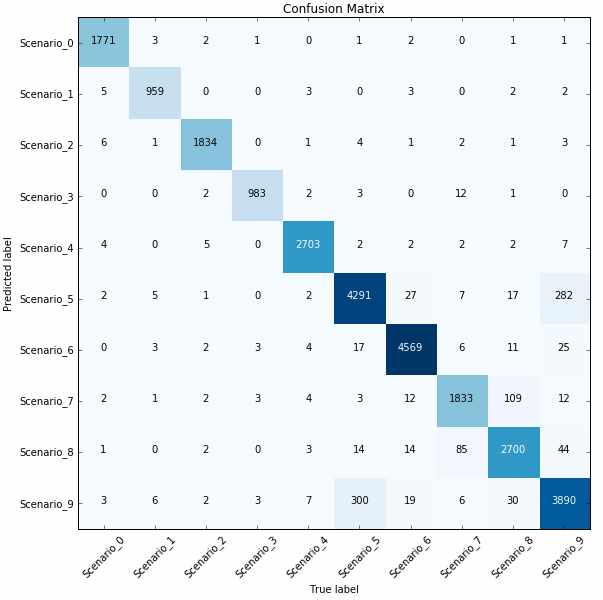
\includegraphics[width=\linewidth]{figures/dtc_unscaled_XL_50}
        \caption{Decision Tree, unscaled, depth=50, trained with whole (XL) dataset}
        \label{fig:knn_4}
    \end{subfigure}
    \caption{Confusion Matrixes for Decision Tree Models}
    \label{fig:confusiondtc}
\end{figure}
\begin{figure}[!htb]
    \captionsetup[subfigure]{justification=centering}
    \centering
    \begin{subfigure}[htb]{0.49\textwidth}
        \centering
        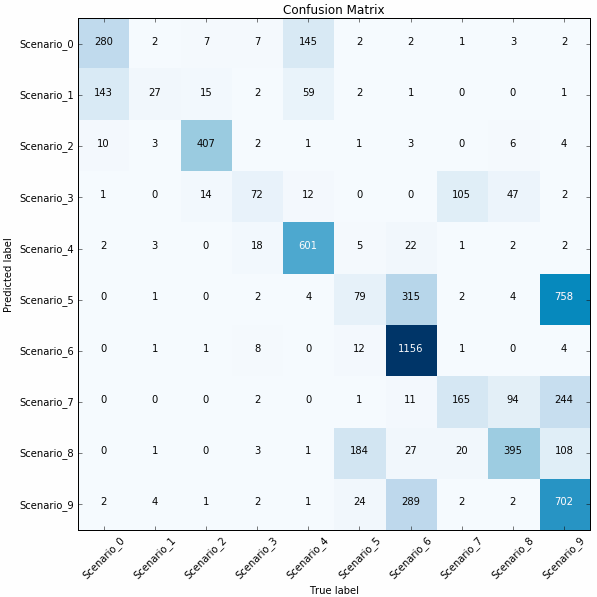
\includegraphics[width=\linewidth]{figures/svc_scaled_S_1}
        \caption{\ac{SVM}, StandardScaled, \(\gamma=2^{-9}\), trained with small (S) dataset}
        \label{fig:knn_2}
    \end{subfigure}
    \begin{subfigure}[htb]{0.49\textwidth}
        \centering
        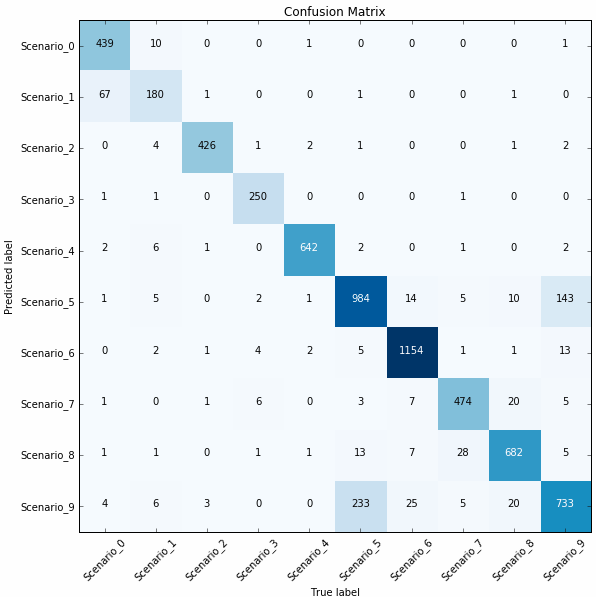
\includegraphics[width=\linewidth]{figures/svc_scaled_S_1e6}
        \caption{\ac{SVM}, StandardScaled, \(\gamma=2^3\), trained with small (S) dataset}
        \label{fig:knn_4}
    \end{subfigure}
    \caption{Confusion Matrixes for \ac{SVM} Models}
    \label{fig:confusionsvc}
\end{figure}
It is also important to notice the clear difference on the number of samples present for each scenario. This is due to the fact that the measurements performed in section~\ref{ch:measure} were based on runtime and not on number of generated samples, and the feature extraction algorithm described in section~\ref{ch:features} generates a different number of samples for each scenario, because of its dependence on the \emph{frame events} generation consequently of the channel occupation and interframe time of arrival itself. A different approach for feature extraction based on a number of features generated is proposed in chapter~\ref{ch:conclusions}.

From these matrices it can be clearly seen, at a first glance, that the K-Nearest algorithm and the decision trees perform quite well regardless of its configuration, having a more populated diagonal in its confusion matrix in comparison with the \ac{SVM} models. Additionally, just a small improvement in the classification accuracy is seen as the complexity and dataset size increases for this model. In general, it is safe to assert that the classification performs generally well for most of the scenarios except scenario 5, where a higher number of false positives, as well as false negatives, is seen for all models, being misclassified as scenario 9. This indicates that the extracted features for these specific scenarios have a noticeable correlation, which is not utterly surprising given that these scenarios share the channel occupation and interframe delay, being different only in the distribution with which the interframe delay is set: deterministic for scenario 5 and stochastic, with Poisson distribution, for scenario 9. This serves as an invitation to determine a feature that confidently sets a difference between them.
\subsection{Image Classification}\label{ch:image_classification}
For the image classification part of this work, a sequential model based on the work of \cite{Paisana2017} was implemented. The basic structure of this model is shown in Fig~\ref{fig:cnn}. As it can be seen, the model is composed of the connection of different layers, each of them with an specific functionality:

\begin{figure}[!htb]
    \centering
      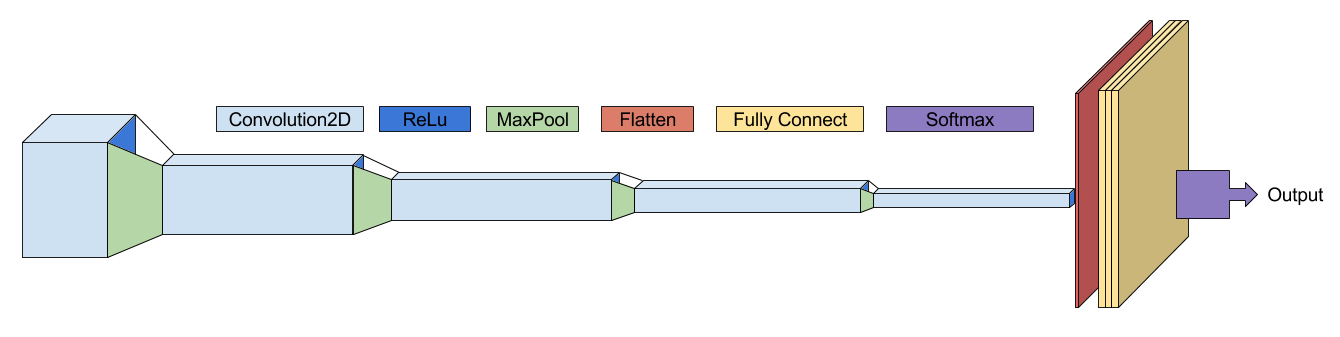
\includegraphics[width=\textwidth]{figures/cnn}
      \caption{Schema of the implemented CNN}
      \label{fig:cnn}
\end{figure}

\begin{itemize}
    \item Convolution2D: this comprises a convolutional kernel. It convolves the input to produce tensors at its output. This is the backbone of the \ac{ConvNet}, as it is the responsible for learning. Here, 2-Dimensional convolutional blocks of kernel size 2x2 are applied, as it is convolving over the area of the input images.
    \item MaxPool: this layer serves its purpose for dimension reduction, which is a form of downsampling. Briefly, it divides the input tensor into 2x2 non-overlapping squares and keeps the largest value present in each of these cells, effectively reducing the size of the representation, which in consequence reduces the number of parameters transitting the network. This has the effect of reducing the number of vector operations as well, making each layer of the network less processing-demandant. Additionally, as parameters are being dropped, this helps to avoid overfitting by disregarding eventual characteristics that are being "memorized". The principle of operation of such layers is shown in Fig~\ref{fig:maxpool}.
        \begin{figure}[!htb]
            \centering
              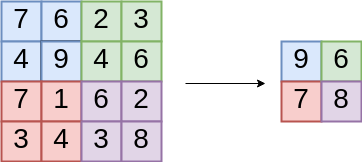
\includegraphics[width=0.4\textwidth]{figures/maxpool}
              \caption{2-D MaxPool}
              \label{fig:maxpool}
        \end{figure}
    \item \ac{ReLu}: this is an activation layer, i.e. a layer that applies a function that defines the type of output depending on its input. In the \ac{ReLu} case, the applied function is \(f(x) =\max(0,x) \), where x is the input of the neuron. Being a non-linear function, this activation increases the nonlinearity of the network without affecting the visual field, as there is no reduction of dimension.
        \begin{figure}[!htb]
            \centering
                \begin{tikzpicture}[scale=0.9]
                    \begin{axis}[
                        xlabel={$x$},
                        ylabel={$f(x)$},
                    ]
                        \addplot[domain=0.001:3,samples=201,purple,thick,smooth]{x};
                        \addplot[domain=-3:0.001,samples=201,purple,thick,smooth]{0};
                    \end{axis}
                \end{tikzpicture}
              \caption{ReLu activation function}
              \label{fig:maxpool}
        \end{figure}
    \item Fully connected layer: as the name states, this layer is connected to each one of the activations of the previous layers. These type of layers are the principle of operation of traditional neural networks, and is in charge of learning the non-linearities that have been propagated throughout the network.
    \item Softmax: this is also an activation layer. It takes vector q of dimension K and compress it together with values that add up to one. The function is given by
        \begin{equation}
            P(q)_i = \frac{e^{q_i}}{\sum_{k=1}^{K} \exp{q_j}}
        \end{equation}

        It can be easily understood that the dimension of the output from this softmax function is the number of labels to classify and that the value of each is the probability of the input sample to belong to that class. Consequently, the classification result is the \( \argmax \) of the function output.
\end{itemize}

The chosen layers and its disposition are strictly related to the input. In this case, the input picture has a 64x64 size, which describes then the height and width of the first layer. The depth is the number of filters that are used for each layer, and it is, to some extent, represented in the extension of the scale of Fig~\ref{fig:cnn}. 5 convolutional layers, with kernel dimensions 2x2, were used in this sequential model, with depths of 48, 128, 192, 192 and 128 filters correspondingly. At the end of the sequential model, 3 fully connected layers with depth 1024, 1024 and 10 were used. The succession of dimension changes of the sequential model and the number of parameters considered in each of the stages of the classification problem is summarized in Table~\ref{table:convnet_summary}. The number of parameters is the number of trainable weights that each layer contains. For a convolutional layer, this is calculated as \( \text{\# parameters} = \text{(depth of input tensor)}\cdot\text{(depth output tensor)}\cdot\text{height}_{kernel}\cdot \text{width}_{kernel} + \text{(depth output tensor)} \). As an example, the calculation for the first layer gives:
\begin{equation*}
    1 \cdot 48 \cdot 2 \cdot 2 + 48 = 240
\end{equation*}

\begin{table}[h!]
    \centering
    \begin{tabular}{|c|c|c|}
        \hline
        \textbf{Layer} & \textbf{Output Shape} & \textbf{\# Parameters} \\
        \hline\hline
        Convolution \# 1 & (63, 63, 48) & 240 \\\hline
        ReLu \# 1 & (63, 63, 48) & 0 \\\hline
        MaxPooling \# 1 & (31, 31, 48) & 0 \\\hline
        Convolution \# 2 & (30, 30, 128) & 24704 \\\hline
        ReLu \# 2 & (30, 30, 128) & 0 \\\hline
        MaxPooling \# 2 & (15, 15, 128) & 0 \\\hline
        Convolution \# 3 & (14, 14, 192) & 98496 \\\hline
        ReLu \# 3 & (14, 14, 192) & 0 \\\hline
        MaxPooling \# 3 & (7, 7, 192) & 0 \\\hline
        Convolution \# 4 & (6, 6, 192) & 147648 \\\hline
        ReLu \# 4 & (6,6, 192) & 0 \\\hline
        MaxPooling \# 4 & (3, 3, 192) & 0 \\\hline
        Convolution \# 5 & (2, 2, 128) & 98432 \\\hline
        ReLu \# 5 & (2,2, 128) & 0 \\\hline
        MaxPooling \# 5 & (1, 1, 128) & 0 \\\hline
        flatten & 128 & 0 \\\hline
        Fully Connected \#1 & 1024 & 132096 \\\hline
        Fully Connected \#2 & 1024 & 1049600 \\\hline
        Fully Connected \#3 & 10 & 10250 \\\hline
        Softmax & 10 & 0 \\\hline
        \hline
    \end{tabular}
    \caption{ConvNet dimensions and Number of Parameters}
    \label{table:convnet_summary}
\end{table}

The sequential model performs an optimization over its error function, for which the optimizer used can be selected. Keras provides a variety of these optimizers, using the approach of the steepest descent optimization over an objective function, \(J(\theta)\) with \(\theta \in \mathbb{R}^{d}\), being \(d\) the dimension of the objective function, by updating the parameters in the opposite direction of the gradient of \(J\), i.e.

\begin{equation}
    \nabla_\theta J(\theta) \text{  w.r.t } \theta, x, y
\end{equation}

A tunable parameter is the learning rate \(\eta\), that determines the size of the steps taken to reach the minimum. For this work, three different optimizers were used and analyzed based on the resulting accuracy of the classification over the test data, as well as its value for error during validation.

\begin{itemize}
    \item Stochastic gradient descent: this algorithm performs a parameter update after each training sample
        \begin{equation}
            \theta = \theta - \eta \cdot \nabla_\theta J(\theta;x^i;y^i)
        \end{equation}
        This optimizer was used in \cite{Paisana2017} and was used as a baseline. The learning rate \(\eta\) was decreased every one-fourth of the total iterations, which in this specific use case was set to 3000. Decreasing the learning rate increases the chance that this optimizer reaches a local minimum.
    \item Adadelta \cite{Zeiler2012a}: this optimizer is based on the Adagrad optimizer \cite{Duchi2011}, which adapts intrinsically its learning rate to the parameters, therefore doing bigger updates for infrequent parameters, and smaller updates for frequent ones. It is proven that this optimizer is more robust than the stochastic gradient descent \cite{Duchi2011} by storing all previous squared gradients and updating accordingly. Adadelta extends this robustness by restricting the amount of accumulated squared gradients to a fixed window, and using this accumulation for its updates.
    \item Adamax: based on the Adaptive Moment Estimation - Adam \cite{Kingma2014}, this optimizer also sets an adaptive learning rate based on the parameters of the objective function. Additionally, to set a fixed window of past squared decays as Adadelta, Adam also keeps an exponentially decaying average of past gradients, which is similar to a momentum \cite{Dahl2013}. Adamax extends Adam functionality by maximizing the norm of the update vector, which leads to a stable behavior.
\end{itemize}

The validation of the models was performed based on the accuracy that these optimizers have during training and testing, the loss factor during the same stages, which is a measure of the error provided by the optimization process. The results are shown in Figs~\ref{fig:sgd}, \ref{fig:adamax} and \ref{fig:adadelta}.

\begin{figure}[!htb]
    \centering
    \begin{subfigure}[htb]{0.49\textwidth}
        \centering
        \begin{tikzpicture}[scale=0.8]
            \begin{axis}[
                xlabel={Iterations},
                ylabel={Loss Factor},
                  ]
                \addplot table [x=epoch, y=loss, col sep=comma, mark=none] {data/sgd.csv};
                \addplot table [x=epoch, y=val_loss, col sep=comma, mark=none] {data/sgd.csv};
                \legend{Training loss, Validation loss}
        \end{axis}
        \end{tikzpicture}
    \end{subfigure}
        \hfill
    \begin{subfigure}[htb]{0.49\textwidth}
        \centering
        \begin{tikzpicture}[scale=0.8]
            \begin{axis}[legend pos=south east,
                xlabel={Iterations},
                ylabel={Accuracy},
                  ]
                \addplot table [x=epoch, y=acc, col sep=comma, mark=none] {data/sgd.csv};
                \addplot table [x=epoch, y=val_acc, col sep=comma, mark=none] {data/sgd.csv};
                \legend{Accuracy, Validation Accuracy}
        \end{axis}
        \end{tikzpicture}
    \end{subfigure}
    \caption{Metrics for Steepest Gradient descent Optimizer}
    \label{fig:sgd}
\end{figure}


\begin{figure}[!htb]
    \centering
    \begin{subfigure}[htb]{0.49\textwidth}
        \centering
        \begin{tikzpicture}[scale=0.8]
            \begin{axis}[
                xlabel={Iterations},
                ylabel={Loss Factor},
                  ]
                \addplot table [x=epoch, y=loss, col sep=comma, mark=none] {data/adamax.csv};
                \addplot table [x=epoch, y=val_loss, col sep=comma, mark=none] {data/adamax.csv};
                \legend{Training loss, Validation loss}
        \end{axis}
        \end{tikzpicture}
    \end{subfigure}
        \hfill
    \begin{subfigure}[htb]{0.49\textwidth}
        \centering
        \begin{tikzpicture}[scale=0.8]
            \begin{axis}[legend pos=south east,
                xlabel={Iterations},
                ylabel={Accuracy},
                  ]
                \addplot table [x=epoch, y=acc, col sep=comma, mark=none] {data/adamax.csv};
                \addplot table [x=epoch, y=val_acc, col sep=comma, mark=none] {data/adamax.csv};
                \legend{Accuracy, Validation Accuracy}
        \end{axis}
        \end{tikzpicture}
    \end{subfigure}
    \caption{Metrics for Adamax Optimizer}
    \label{fig:adamax}
\end{figure}

\begin{figure}[!htb]
    \centering
    \begin{subfigure}[htb]{0.49\textwidth}
        \centering
        \begin{tikzpicture}[scale=0.9]
            \begin{axis}[
                xlabel={Iterations},
                ylabel={Loss Factor},
                  ]
                \addplot table [x=epoch, y=loss, col sep=comma, mark=none] {data/adadelta.csv};
                \addplot table [x=epoch, y=val_loss, col sep=comma, mark=none] {data/adadelta.csv};
                \legend{Training loss, Validation loss}
        \end{axis}
        \end{tikzpicture}
    \end{subfigure}
    \hfill
    \begin{subfigure}[htb]{0.49\textwidth}
        \centering
        \begin{tikzpicture}[scale=0.9]
            \begin{axis}[legend pos=south east,
                xlabel={Iterations},
                ylabel={Accuracy},
                  ]
                \addplot table [x=epoch, y=acc, col sep=comma, mark=none] {data/adadelta.csv};
                \addplot table [x=epoch, y=val_acc, col sep=comma, mark=none] {data/adadelta.csv};
                \legend{Accuracy, Validation Accuracy}
        \end{axis}
        \end{tikzpicture}
    %}
    \end{subfigure}
    \caption{Metrics for Adadelta Optimizer}
    \label{fig:adadelta}
\end{figure}

From these plots, it can clearly be seen that SGD takes a greater number of iterations to reach its maximum accuracy as well as its minimum loss factor in comparison with Adamax and Adadelta. With respect to their comparative accuracies, it is not conclusive that one of the optimizers provide a better result. The maximum and final values of the accuracies of these models are shown in Table~\ref{table:convnet_accs}, whilst the minimum and final values for the loss factor is shown in Table~\ref{table:convnet_loss}.

\begin{table}[!ht]
  \centering
    \begin{tabular}{| >{\centering\arraybackslash}m{5em}| >{\centering\arraybackslash}m{7em}| >{\centering\arraybackslash}m{7em}| >{\centering\arraybackslash}m{7em}| >{\centering\arraybackslash}m{7em}|}
    \cline{2-5}
      \multicolumn{1}{c|}{} & Max Training Accuracy (Iter) & Final Training Accuracy & Max Validation Accuracy (iter) & Final Validation accuracy \\ \hline
      SGD & 99\% (2411)   & 98\%   & 90\% (981) & 81\%  \\ \hline
      Adamax & 92\% (2997)   & 88\%   & 87\% (2679) & 77\%  \\ \hline
      Adadelta & 100\%(2012)   & 99.6\%   & 89\% (489) & 85\%  \\ \hline
  \end{tabular}
    \caption{Maximum and Final Accuracies for ConvNets with various optimizers}
    \label{table:convnet_accs}
\end{table}


\begin{table}[!ht]
  \centering
    \begin{tabular}{| >{\centering\arraybackslash}m{5em}| >{\centering\arraybackslash}m{7em}| >{\centering\arraybackslash}m{7em}| >{\centering\arraybackslash}m{7em}| >{\centering\arraybackslash}m{7em}|}
    \cline{2-5}
      \multicolumn{1}{c|}{} & Min Training Loss (Iter) & Final Training Loss & Min Validation Loss (iter) & Final Validation Loss \\ \hline
  SGD & 0.625 (2866)   & 0.64   & 0.863 (861) & 1.134  \\ \hline
      Adamax & 0.24 (2997)   & 0.37   & 0.47 (1150) & 0.93  \\ \hline
      Adadelta & 0.03 (2998)   & 0.04   & 0.4 (297) & 0.74  \\ \hline
  \end{tabular}
    \caption{Maximum and Final Loss Factor for ConvNets with various optimizers}
    \label{table:convnet_loss}
\end{table}

The low values for losses as well as high values for accuracies in the training process do not come as a surprise, but it is the iteration where they are reached what is significant to be analyzed, as they state the rate of convergence of each of the optimizers. For the training phase, it is also expected that these values are constantly increasing along the whole process, as the model keeps learning from the data and fits to it. Therefore, it is of special interest to focus the attention to the validation part. Regarding the accuracy value, it is not conclusive to determine an algorithm that outperforms the others. Additionally, an accuracy greater than 87\% for all the optimizers is satisfactory, keeping in mind that these models are trained with spectrograms with SNR as low as -5dB, where the \ac{PU} signal is well below the noise level. It is clear that the rate of convergence of Adadelta surpasses the performance of the other optimizers, for both the maximum validation accuracy and the minimum validation loss, which states that using early stop techniques allows having a satisfactory model with short training time. More insights about the early stop techniques are given in the following chapter, where it will be clear why the maximum validation accuracy and minimum validation loss are important values to be considered.

Looking carefully at the loss factor plots for validation, a clear tendency of the increase of this parameter at the end of the iterative process can be seen for the Adamax and Adadelta optimizers, which is an indication of overfitting. Although not clear from the plots, SGD also shows overfitting behavior to some extent, as it can be seen in the noticeable difference on the maximum accuracy vs the final accuracy in table~\ref{table:convnet_accs}.


  \acresetall
\chapter{Live implementation in GNURadio}\label{chapter:live} \label{ch:live}

A live implementation of the scenario classification has been implemented using GNURadio. The models have been trained with the procedures explained in previous chapters and afterward its persistence is achieved using the sklearn library joblib for the feature-based learning and the library PyH5 for the spectrogram based learning.

The selection of the saved models is crucial for the good performance of the application. For the feature-based learning, the models with the best trade-off between validation accuracy and prediction time have been chosen. The selected models are:

\begin{itemize}
    \item K-nearest neighbors with 4 neighbors, trained with the whole (XL) unscaled dataset.
    \item A Decision tree with a tree depth=50, trained with the whole (XL) scaled dataset using a standard scaler.
    \item \ac{SVM} with an RBF complexity of \(\gamma=2^3\), trained with the medium (M) scaled dataset using a standard scaler.
\end{itemize}

For the spectrogram-based learning, an interesting technique is used for choosing the best fit for the real-time implementation. Keras provides routines for saving the model after the total of iterations is done, where one can assume that the model, after extensive training, will have an improving performance with increasing iteration number. However, a long training time can lead to overfitting of the model as seen at the end of section~\ref{ch:image_classification}. Two alternatives to avoid this are provided based on a constant callback of the accuracy and loss parameters. These alternatives are:

\begin{itemize}
    \item Early stopping: a monitored quantity can be selected from the accuracies or losses, and a range of improvement is set by the designer. Constantly, the selected value is checked, and everytime that it reaches a better performance a model's persistence is saved to disk. If there is no improvement in an arbitrary number of iterations thereafter, the process is stopped and the persistence of the model at the last iteration can also be saved to disk.
    \item Model Checkpoint: similarly to early stopping, a monitored quantity is selected, and the best model's persistence with respect to that quantity is saved to disk. However, the whole training process is run to completion, where the persistence of the model at the last iteration can also be saved to disk as well.
\end{itemize}

In this work model checkpoint was selected for model persistence, as it provides the capability of saving the best model with respect to a parameter as well as allowing the observation of the whole process by the cost of training times. The validation loss was selected as monitored quantity, as it represents how different was the predicted data to the training data, and considering that there is no significant improvement of accuracy after a couple hundreds of iterations for any of the models.

Simple blocks have been written to serve as a wrapper for the trained models, and a comparative setup with the implementation used at the DySpan Spectrum Challenge 2017 is carried out. As a first approach, the classification probabilities is extracted in real time. These probabilities state how certain is each of the algorithms at making a decision. For plotting, a modified "QT Time Raster" block is used, to see in the x-axis, ordinally, the possible scenarios from scenario 0 to 9, and the y-axis updates constantly to show outputs of the classifiers. It is important to notice that none of these axes reflect time directly, as it will become clear shortly. For testing, the \ac{PU} transmitter is set to send its packets using the scenarios increasingly for a duration of 2 seconds each. Additionally, different values of \ac{PU} transmission power have been used to determine the performance of the implemented machine learning algorithms facing different values of SNR. Fig~\ref{fig:prob_snr_15} shows these probability plots for an SNR=15dB.

\begin{figure}[!htb]
    \centering
      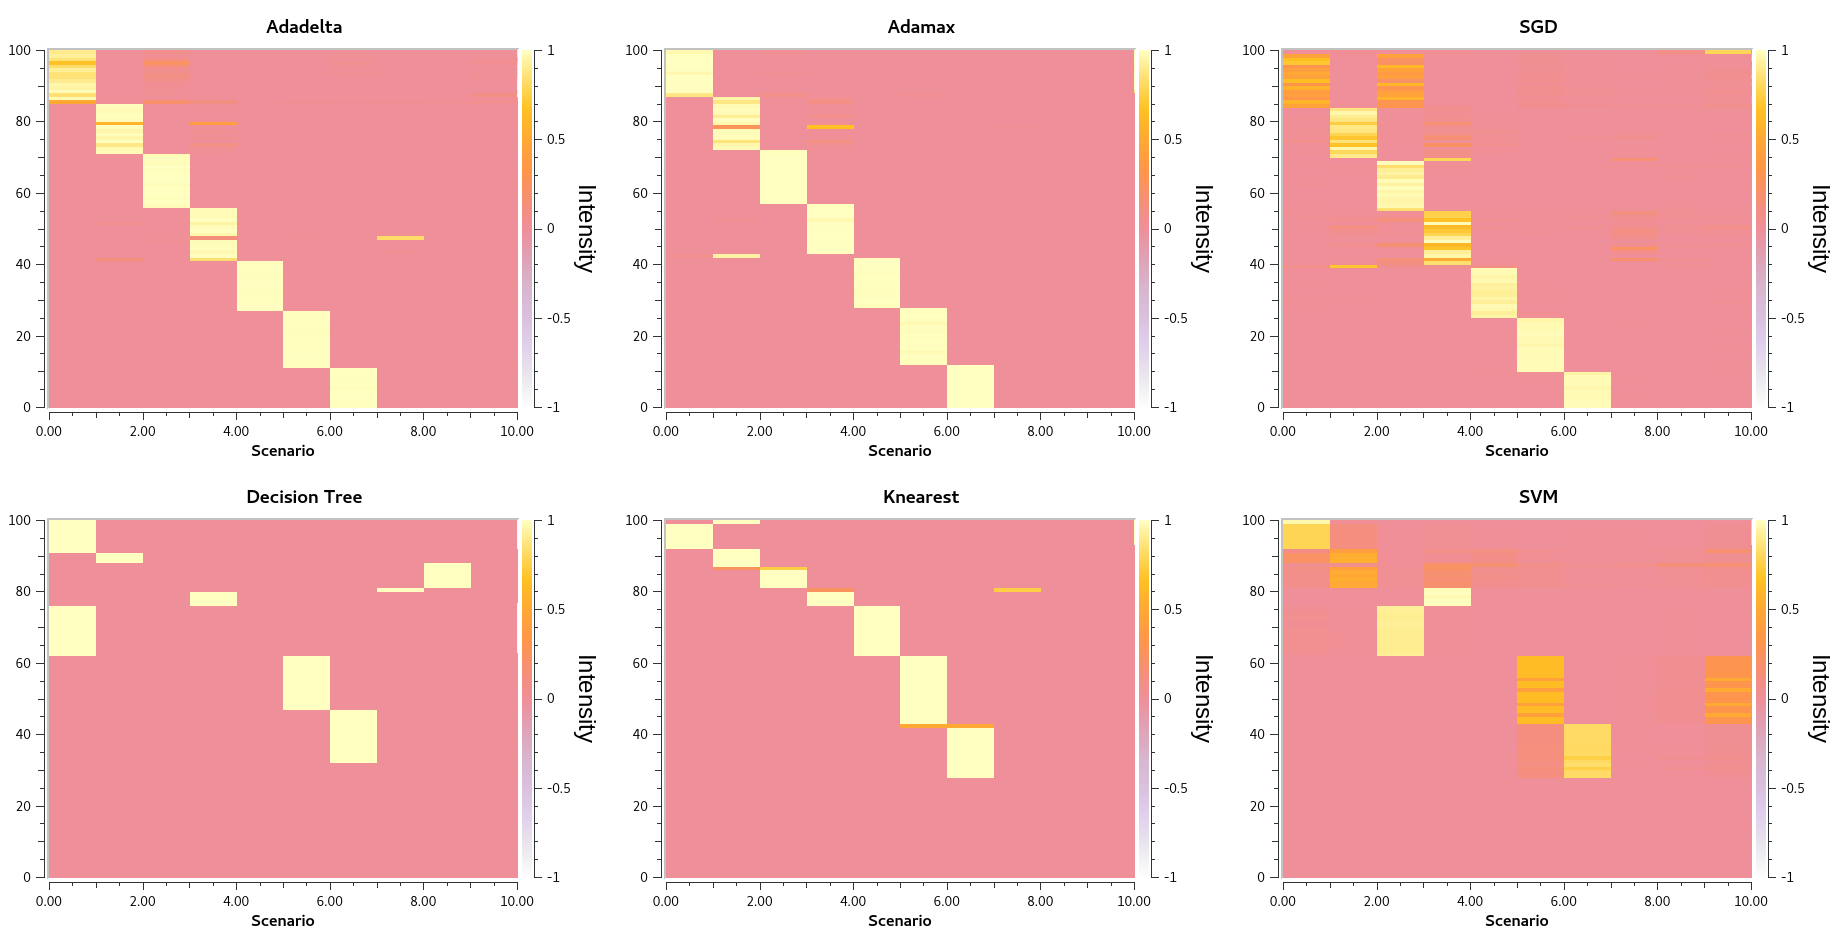
\includegraphics[width=\textwidth]{figures/prob_snr_15}
      \caption{Decision certainty for an SNR=15dB}
      \label{fig:prob_snr_15}
\end{figure}

The high intensity on these plots is represented with a lighter color and means a higher probability/certainty of a decision. In the top row the spectrogram-based algorithms are shown, and it can be seen that they show a consistent classification for each scenario every 2 seconds. Furthermore, the certainty of Adadelta and Adamax is clearer at the moment of making a decision vs. the certainty of SGD. However, this has little effect in the final result, as still the right scenario has a higher probability and is correctly classified, as seen in Fig~\ref{fig:scn_snr_15}. The row on the bottom shows the feature-based learning algorithms. On first instance it could be understood that they are not classifying correctly the scenarios, as a definite staircase-like fashion, as for the top row, is intuitively expected. However, it is important to notice that the nature of these classification models is different: it is feature based, while the top row is, so to say, sample based. What this means is that the top row classifies scenarios on the go based solely on the input data, whilst the bottom row classifies based on the frame events generated by the blocks described in Fig~\ref{fig:frame_events}. These frame events vary in quantity based on the number of frames that the \ac{PU} is transmitting, reason why in Fig~\ref{fig:scn_snr_15} the classified scenarios show to be longer for scenario 6 (high packet rate) than, for example, scenario 7 (low packet rate). This explains the difference on the output patterns.

\begin{figure}[!htb]
    \centering
      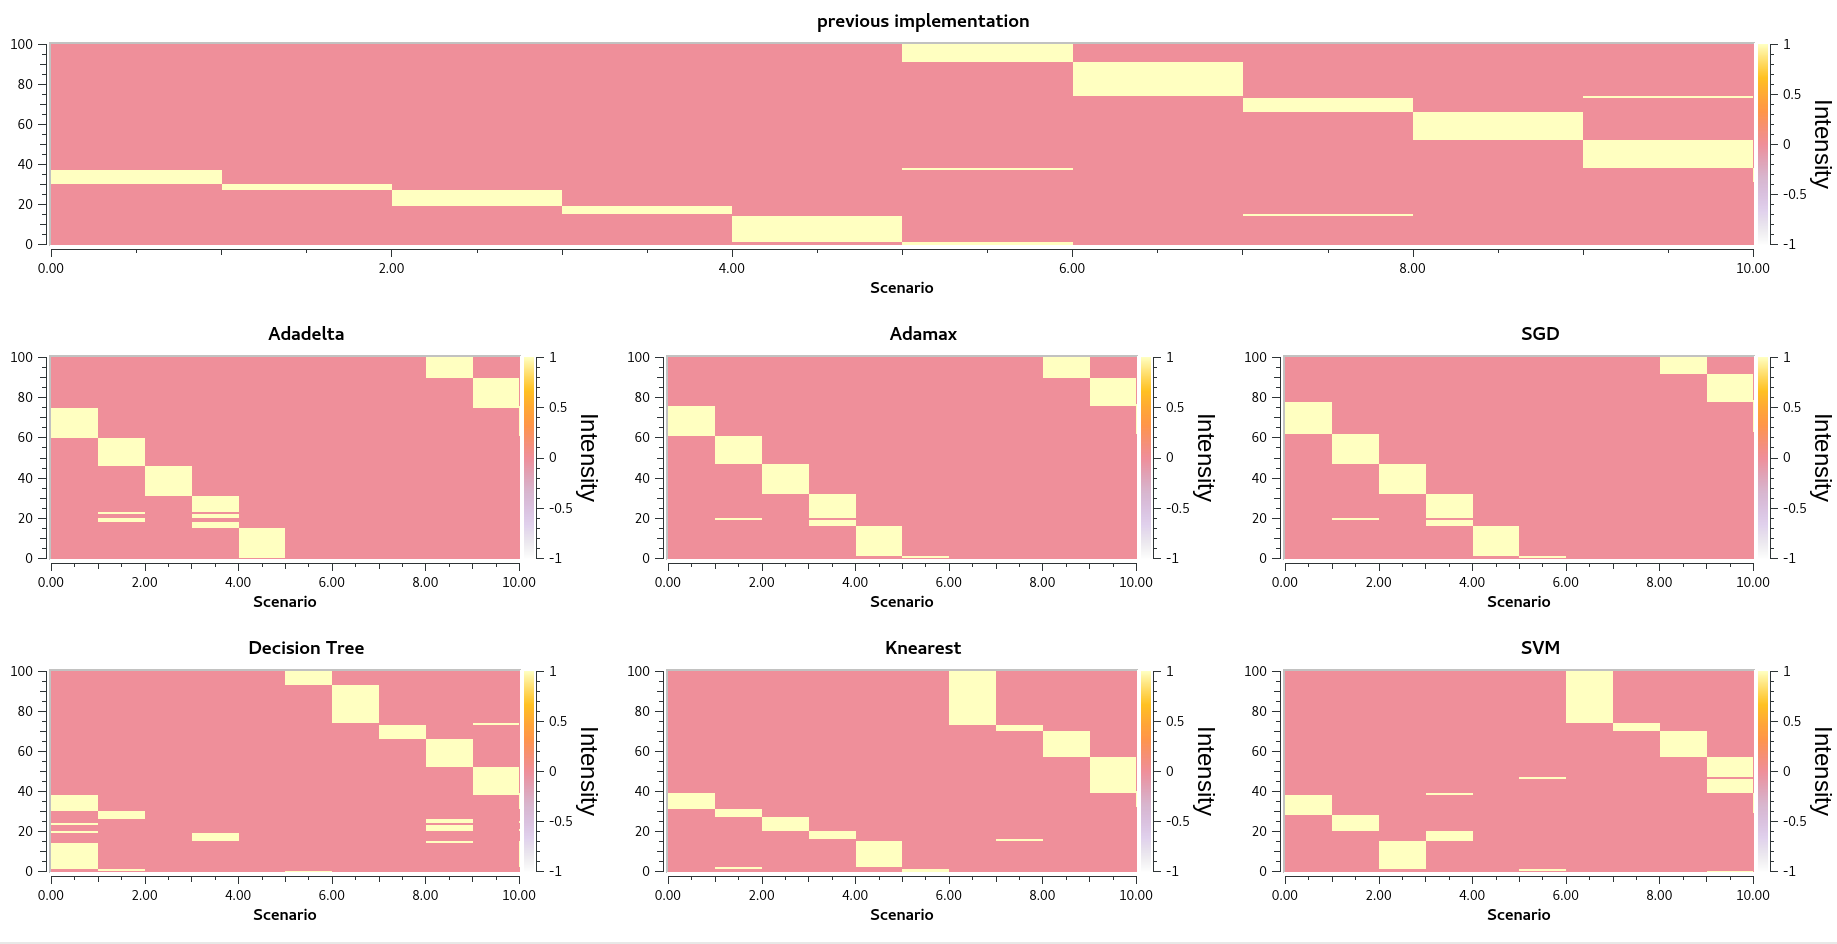
\includegraphics[width=\textwidth]{figures/scn_snr_15}
      \caption{Classified scenario for an SNR=15dB}
      \label{fig:scn_snr_15}
\end{figure}

In Fig~\ref{fig:scn_snr_15}, and in upcoming scenario classification figures, the implementation used in the DySpan Spectrum Challenge 2017 is plotted in the top row, moving the rows from Fig~\ref{fig:prob_snr_15} one position down. It can be seen that the pattern is alike to the feature-based classifiers, as they use the same features and frame events.

Additional plots for the decision probability and classified scenario are shown for SNR=10dB in Figs~\ref{fig:prob_snr_10}, \ref{fig:scn_snr_10}, SNR=5dB in Figs~\ref{fig:prob_snr_5}, ~\ref{fig:scn_snr_5} and SNR=0dB in Figs~\ref{fig:prob_snr_0}, \ref{fig:scn_snr_0}. An evident increase in the uncertainty can be seen with a decrease of the SNR, which is expected. Nevertheless, the spectrogram-based classifiers continue to have a remarkable performance even with low values of \ac{PU} transmit power. An important remark that cannot be seen in the pictures is that for SNR=5dB and below the frequency with which the frame events are generated decreases, given that they depend on detection of \ac{PU} energy. Because of this fact, all feature-based classifiers stop generating outputs consistently, until the point they just stop classifying (or generating outputs whatsoever). This sets a clear advantage for the spectrogram-based classifiers, as they are independent of the \ac{PU} transmission power.

\begin{figure}[!htb]
    \centering
      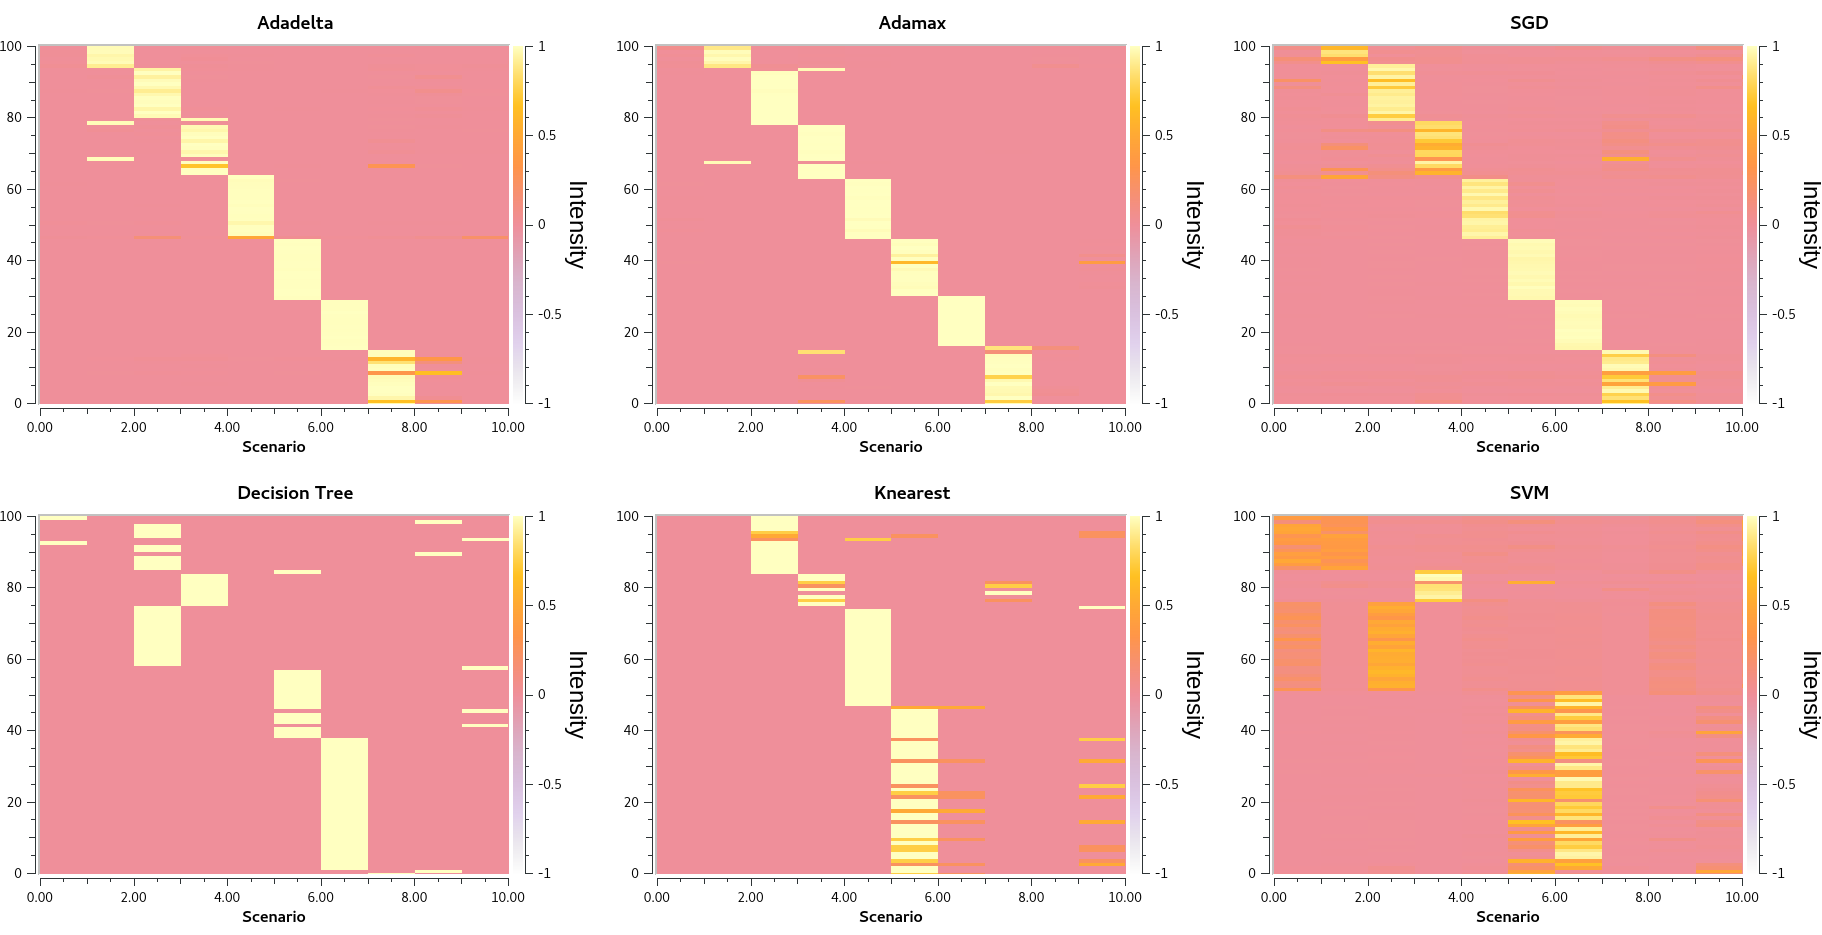
\includegraphics[width=\textwidth]{figures/prob_snr_10}
      \caption{Decision certainty for an SNR=10dB}
      \label{fig:prob_snr_10}
\end{figure}

\begin{figure}[!htb]
    \centering
      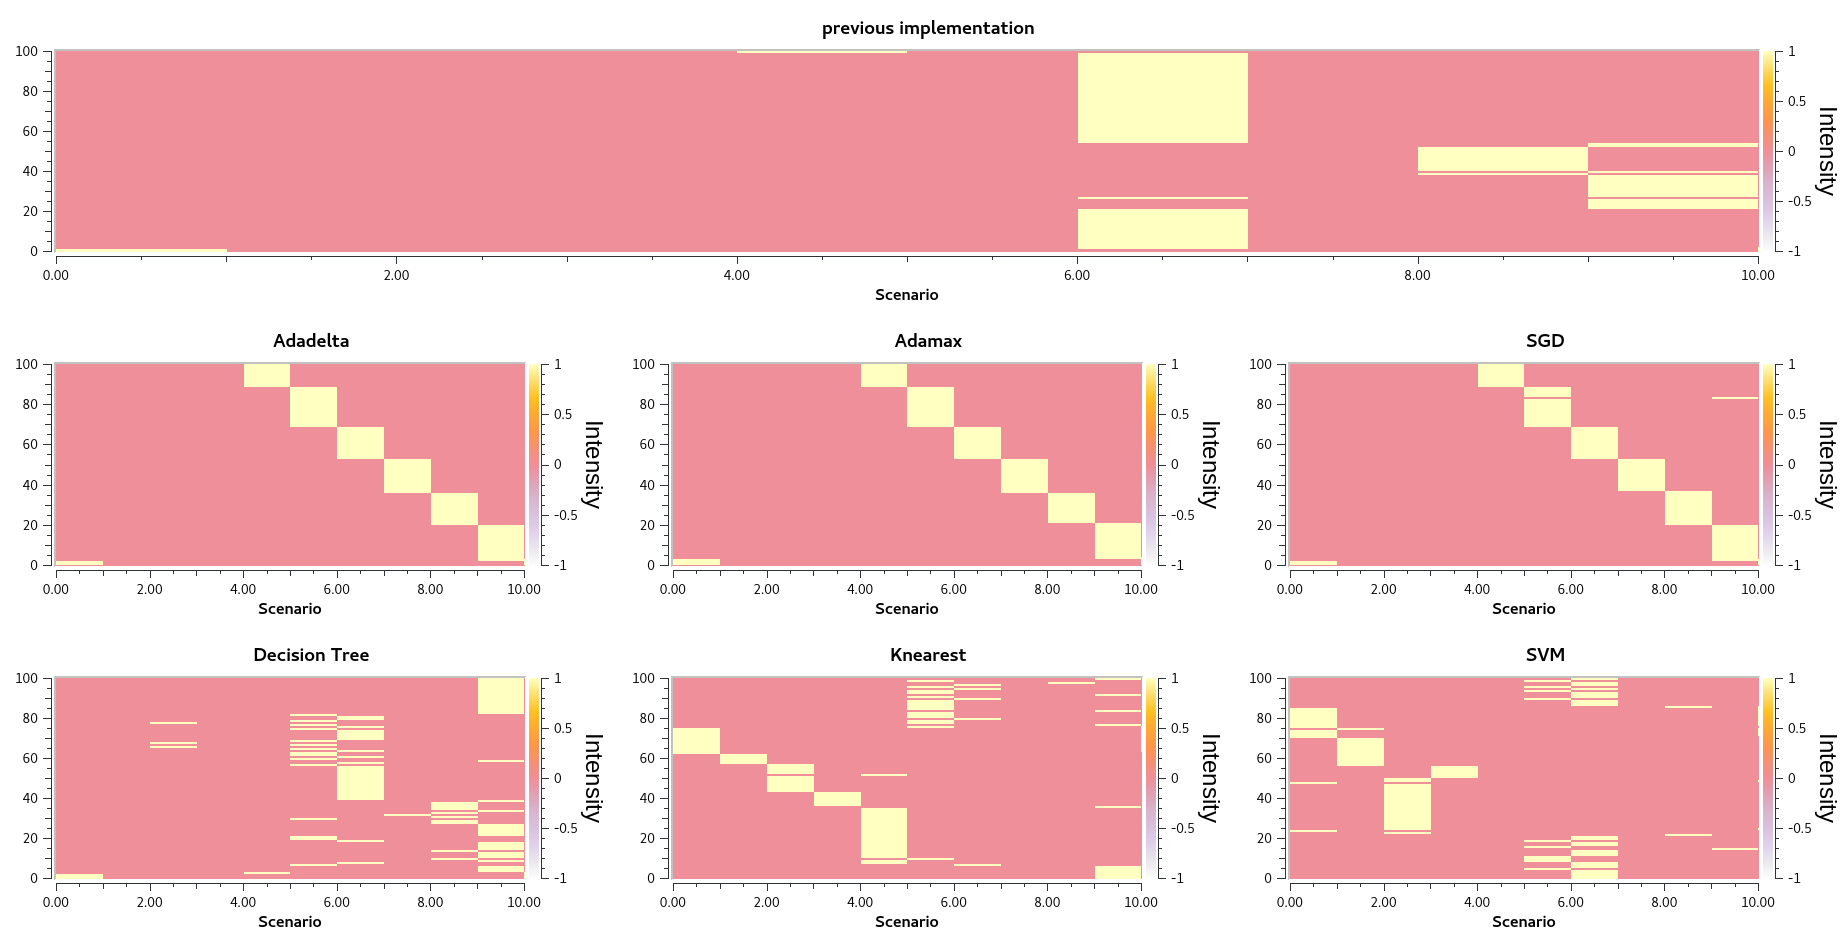
\includegraphics[width=\textwidth]{figures/scn_snr_10}
      \caption{Classified scenario for an SNR=10dB}
      \label{fig:scn_snr_10}
\end{figure}

\begin{figure}[!htb]
    \centering
      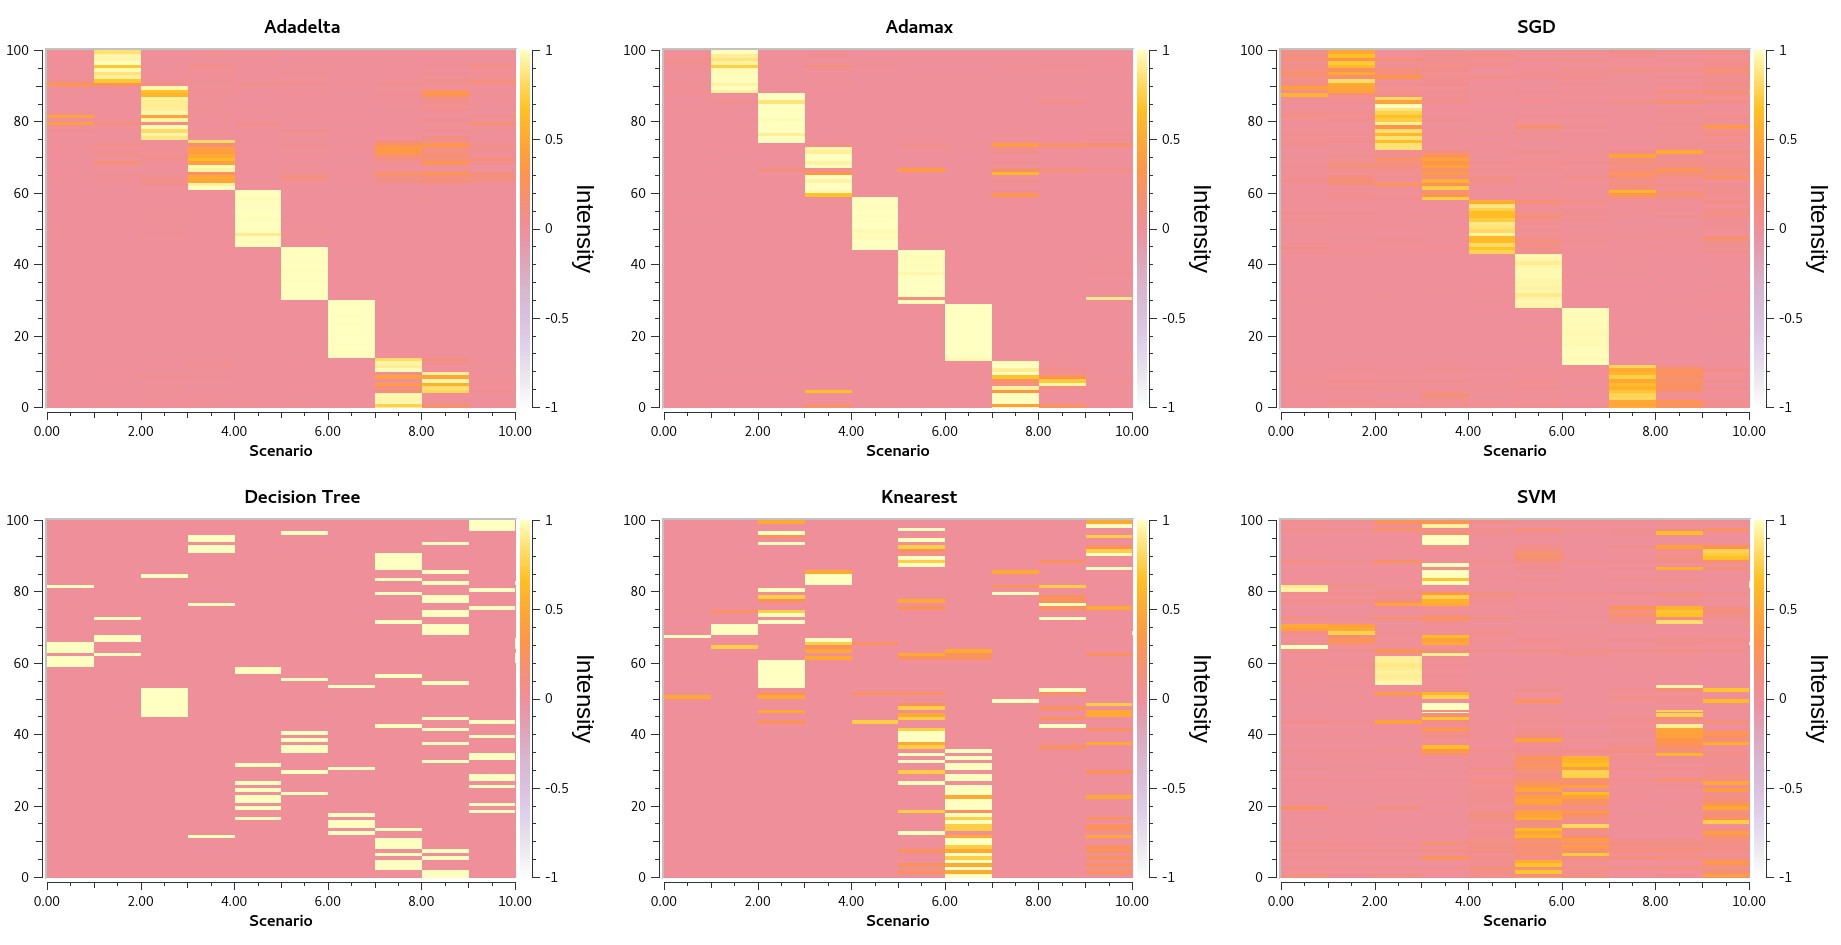
\includegraphics[width=\textwidth]{figures/prob_snr_5}
      \caption{Decision certainty for an SNR=5dB}
      \label{fig:prob_snr_5}
\end{figure}

\begin{figure}[!htb]
    \centering
      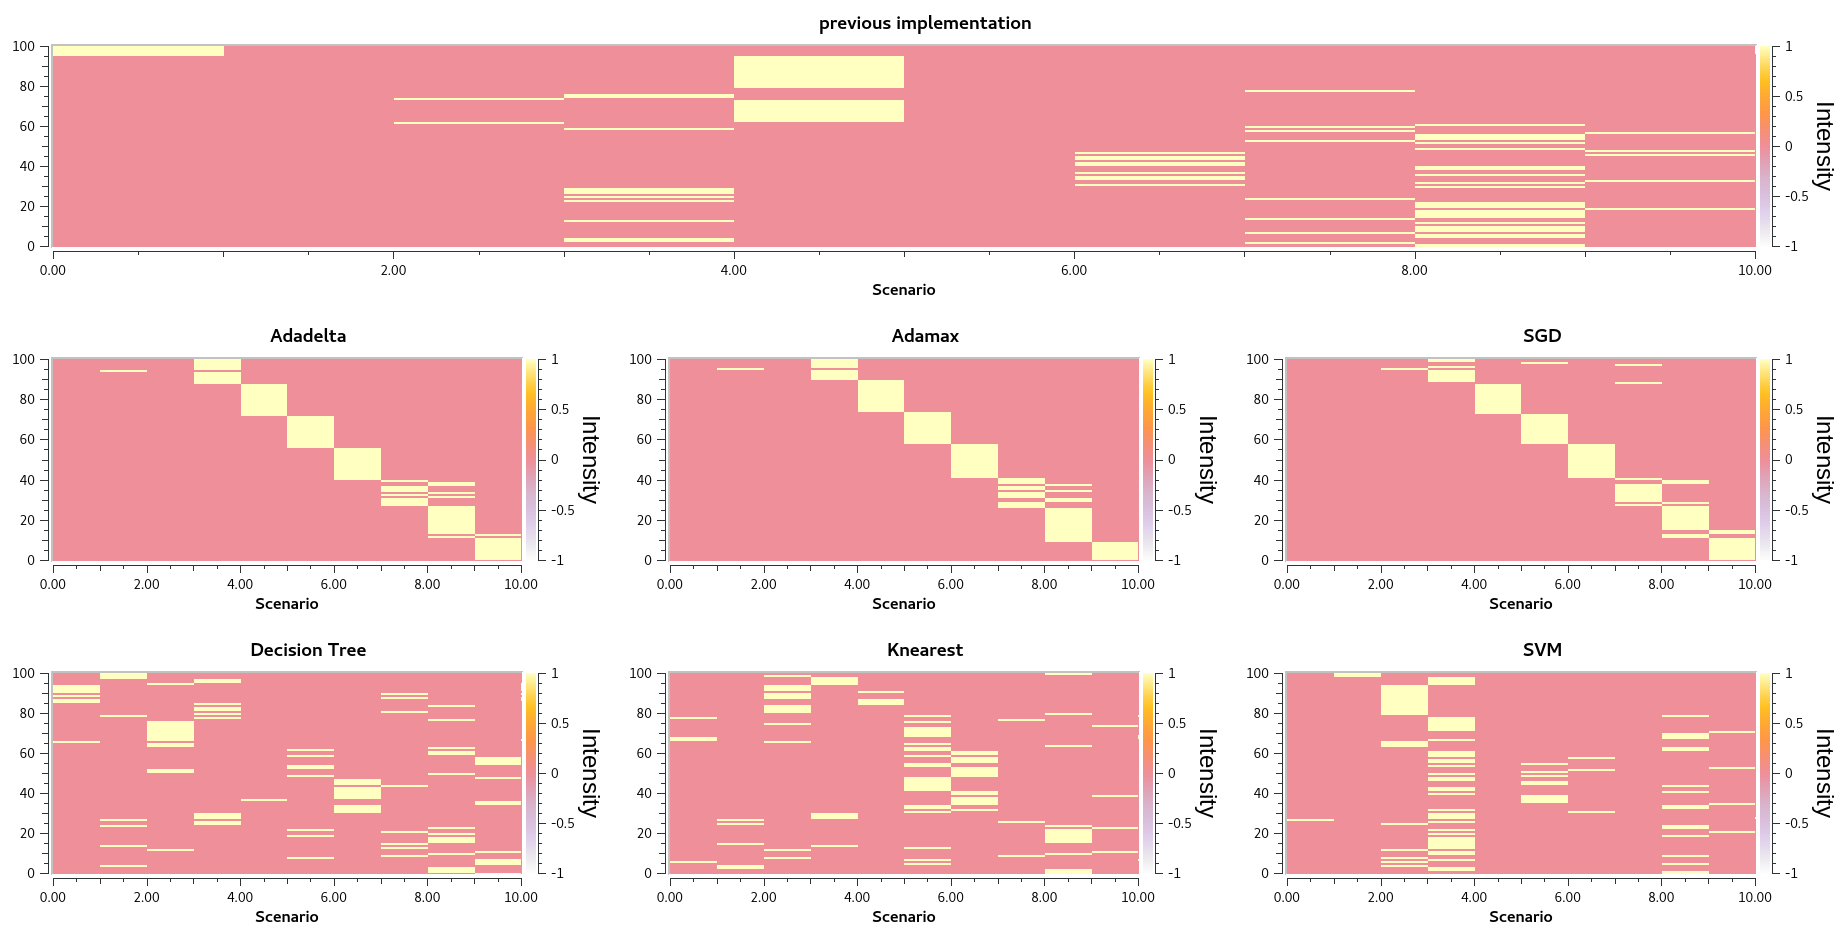
\includegraphics[width=\textwidth]{figures/scn_snr_5}
      \caption{Classified scenario for an SNR=5dB}
      \label{fig:scn_snr_5}
\end{figure}

\begin{figure}[!htb]
    \centering
      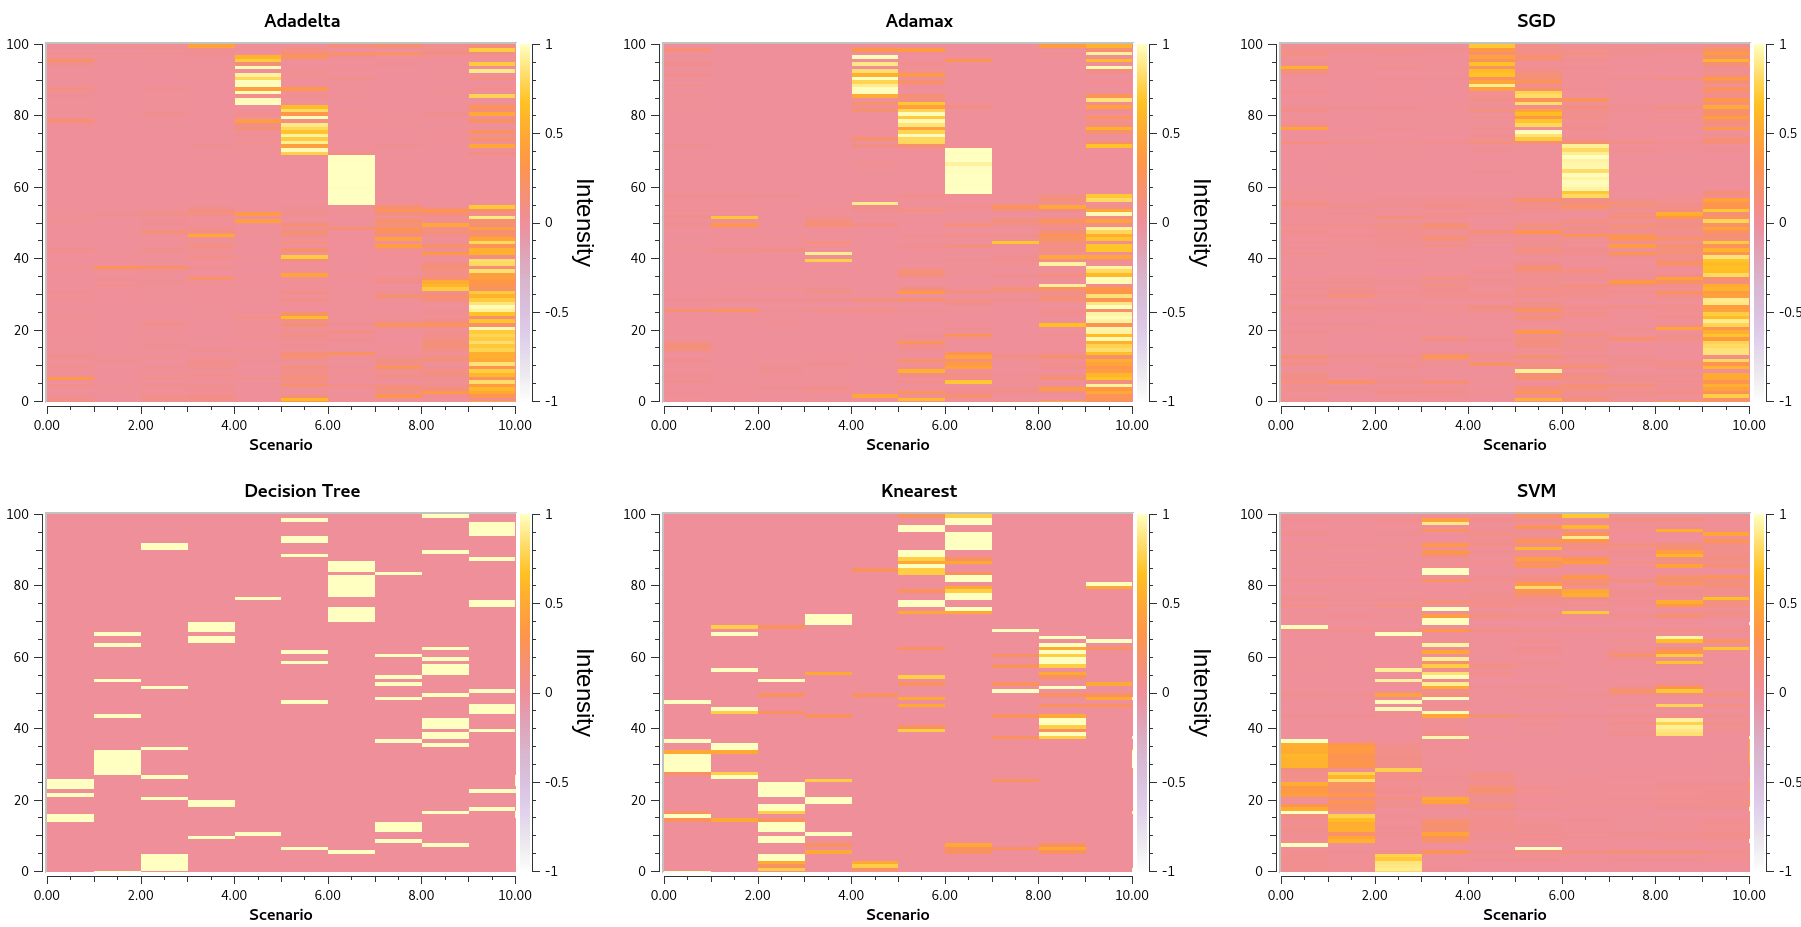
\includegraphics[width=\textwidth]{figures/prob_snr_0}
      \caption{Decision certainty for an SNR=0dB}
      \label{fig:prob_snr_0}
\end{figure}

\begin{figure}[!htb]
    \centering
      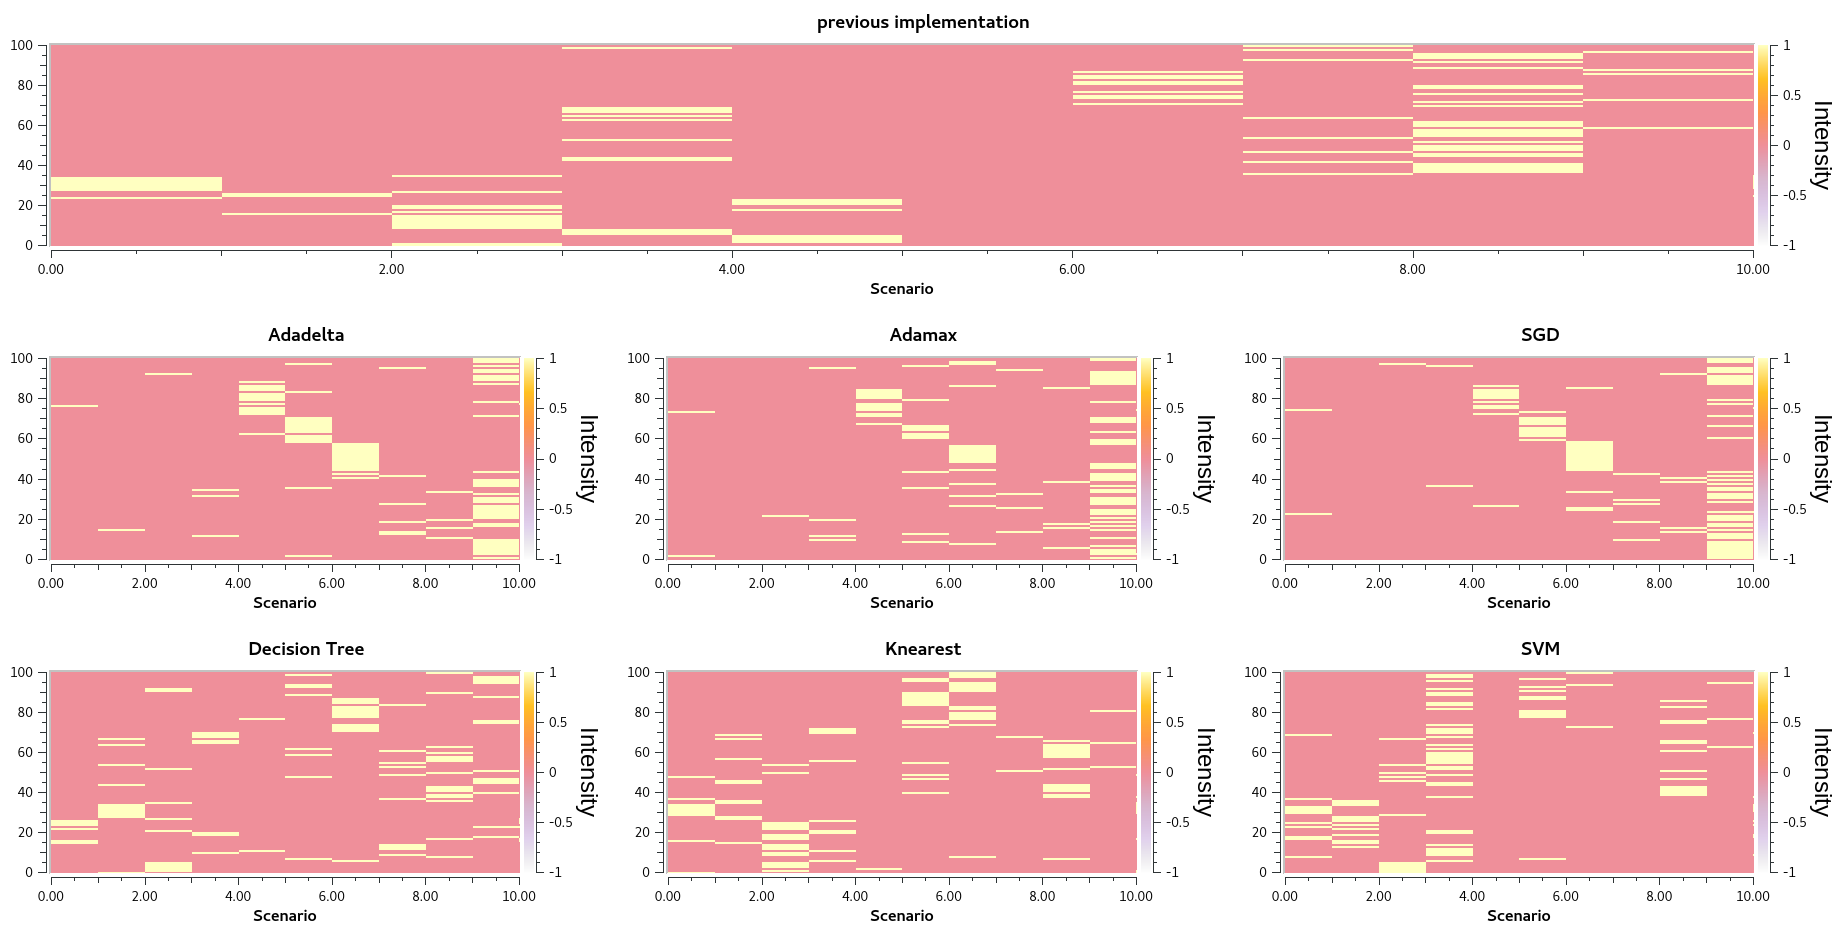
\includegraphics[width=\textwidth]{figures/scn_snr_0}
      \caption{Classified scenario for an SNR=0dB}
      \label{fig:scn_snr_0}
\end{figure}


%  \acresetall
% This is an example chapter from 'Polar Codes for Software Radio'. Do not use it but delete it! It serves as an example!
\chapter{System model}\label{chapter:systemmodel}
Polar codes are defined for a specific system model.
The objective of this chapter is to introduce the key concepts.
Notations are introduced and important terms are revisited in order to refer to them.

\section{Key channel coding concepts}
The system model used throughout this thesis follows the remarks in \cite{Richardson:2008:MCT} and \cite{polar:arikan09}.
It is intended to define the domain for which polar codes are developed.

The objective of channel coding is to transmit information from a source to a sink over a point-to-point connection with as few errors as possible.
A source wants to transmit binary data  $u \in \mathcal{U} = \{0, 1\}$ to a sink where $u$ represents one draw of a binary uniformly distributed random variable.
The source symbols are encoded, transmitted over a channel and decoded afterwards in order to pass an estimate $\hat{u}$ to a sink.

This thesis uses a common notation for vectors which is introduced here shortly.
A variable $x$ may assume any value in an alphabet $x \in \mathcal{X}$.
Multiple variables are combined into a vector $x^N = (x_0, \dots , x_{N-1})$ of size $N$ with its alphabet $x^N \in \mathcal{X}^N$.
A subvector of $x^N$ is denoted $x_i^j = (x_i, \dots, x_{j-1})$ where $0 \leq i \leq j \leq N$.
A vector where $i=j$ is an empty vector.
A vector $x^N$ may be split into even and odd subvectors which are denoted $x_{0,e}^{2n} = (x_0, x_2, \dots, x_{2n-2})$, $x_{0,o}^{2n} = (x_1, x_3, \dots, x_{2n-1})$.
This numbering convention is in accordance with \cite{dijkstra:zerocounting}, where the author makes a strong point for this exact notation and some papers on polar codes follow it too, e.g. \cite{polar:talvardy:howtoCC}.


\subsection{Encoder}
The encoder takes a frame $u^k$ and maps it to a binary codeword $x^N$, where $k$ and $N$ denote the vector sizes of a frame and a codeword respectively with $k \leq N$.
An ensemble of all valid codewords for an encoder is a code $\mathcal{C}$.
It should be noted that $|\mathcal{C}| = |\mathcal{X}^N|$ must hold in order for the code to be able to represent every possible frame.

Not all possible symbols from $\mathcal{X}^N$ are used for transmission.
The difference between all possible codewords $2^N$ and used codewords $2^k$ is called redundancy.
With those two values, the code rate is defined as $R = \frac{k}{N}$.
It is a measure of efficient channel usage.

The encoder is assumed to be linear and to perform a one-to-one mapping of frames to codewords.
A code is linear if $\alpha x + \alpha' x' \in \mathcal{C}$ for $\forall x, x' \in \mathcal{C}$ and $\forall \alpha, \alpha' \in \mathbb{F}$ hold.
It should be noted that all operations are done over the Galois field GF(2) or $\mathbb{F} = \{0, 1\}$ if not stated otherwise.
Then the expression can be simplified to 
\begin{equation}
 x + x' \in \mathcal{C} \quad \textrm{for} \quad \forall x, x' \in \mathcal{C}.
\end{equation}
A linear combination of two codewords must yield a codeword again.

For linear codes it is possible to find a generator matrix $G \in \mathbb{F}^{k \times N}$ and obtain a codeword from a frame with $x^N = u^k G^{k \times N}$.
All linear codes can be transformed into systematic form $G = I_k P$.
$I_k$ is a $k \times k$ dimensional identity matrix.
If $G$ is systematic, all elements of a frame $u^k$ are also elements of the codeword $x^N$.
Also, a parity check matrix $H = -P^T I_{N-k}$ with dimensions $(N-k) \times N$ can be calculated from $G$.
A parity check matrix satisfies $\forall x \in \mathcal{C}: H x^T = 0^T $.
Thus, a parity check matrix can be used to verify correct codeword reception and furthermore error correction may be performed.
Error correction with $H$ may be done, e.g. syndrome decoding.

A code can be characterized by the minimum distance between any two codewords.
In order to obtain this value we use the Hamming distance.
This distance $d(v^N,x^N)$ equals the number of positions in $v^N$ that differ from $x^N$.
Minimum distance of a code is than defined by $d(\mathcal{C}) = \min\{d(x,v): x,v \in \mathcal{C}, x \neq v\}$.
For linear codes this can be simplified to comparing all codewords to the zero codeword $d(\mathcal{C}) = \min\{d(x,0): x \in \mathcal{C}, x \neq 0\}$ which is called Hamming weight.

\subsection{Channel model}\label{sec:channel_model}
Channel coding relies on a generic channel model.
Its input is $x \in \mathcal{X}$ and its distorted output is $y \in \mathcal{Y}$.
A channel is denoted $W: \mathcal{X} \rightarrow \mathcal{Y}$ along with its transition probability $W(y|x), x \in \mathcal{X}, y \in \mathcal{Y}$.
A \ac{DMC} does not have memory, thus every symbol transmission is independent from any other.
Combined with a binary input alphabet it is called a \ac{BDMC}.
For a symmetric channel model, $P(y|1) = P(-y|-1)$ must hold for an output alphabet $y \in \mathcal{Y}, \mathcal{Y} \subset \mathbb{R}$ \cite{Richardson:2008:MCT}.
Assuming symmetry for a \ac{BDMC} leads to a symmetric \ac{BDMC}.
In Sec. \ref{theory:channels} several examples of such channels are discussed.

This channel concept may be extended to vector channels.
A vector channel $W^N$ corresponds to $N$ independent uses of a channel $W$ which is denoted as $W^N : \mathcal{X}^N \rightarrow \mathcal{Y}^N$.
Also, vector transition probabilities are denoted $W^N(y^N|x^N) = \prod_{i=0}^{N-1} W(y_i|x_i)$.

\subsection{Decoder}
A decoder receives a possibly erroneous codeword $y$ and checks its validity by asserting $H y^T = 0^T$, thus performing error detection.
A more sophisticated decoder tries to correct errors by using redundant information transmitted in a codeword.
An optimal decoder strategy is to maximize the a-posteriori probability.
Given the probability of each codeword $P(x)$ and the channel transition probability $P(y|x)$, the task at hand is to find the most likely transmitted codeword $x$ under the observation $y$, $P(x|y)$.
This is denoted
\begin{equation}
 \hat{x}^{MAP} = \argmax_{x \in \mathcal{C}} p(x|y) = \argmax_{x \in \mathcal{C}} p(y|x) \frac{p(x)}{p(y)} = \argmax_{x \in \mathcal{C}} p(y|x) p(x)
\end{equation}
with Bayes' rule.
Assume every codeword is transmitted with same probability $P(x^{(i)}) = P(x^{(j)}), \; \forall x^{(i)}, x^{(j)} \in \mathcal{C}$.
This simplifies the equation and yields a \ac{ML} decoder
\begin{equation}
 \hat{x} = \argmax_{x \in \mathcal{C}} p(y|x)
\end{equation}
which estimates the most likely codeword to be transmitted given a received possibly erroneous codeword \cite{Richardson:2008:MCT}.
This decoding principle could be employed in conjunction with the Hamming distance and thus yield $\hat{x} = \argmin_{x \in \mathcal{C}} d(x, y)$.
In conclusion the task at hand is to find a code which inserts redundancy intelligently, so a decoder can use this information to detect and correct transmission errors.

\subsection{Asymptotically good codes}\label{theory:repetition_code}
A repetition code is a very simple code which helps clarify certain key concepts in the channel coding domain.
Assume the encoder and decoder use a repetition code.
For example a repetition code with $k=1$ and $N = 3$ has two codewords $\mathcal{C} = \{000, 111\}$.
Thus in this example $R=\frac{1}{3}$.
We can also obtain its generator and parity check matrices.
\begin{equation}
 G = \begin{pmatrix} 1 & 1 & 1 \end{pmatrix},\qquad H = \begin{pmatrix} 1 & 1 & 0 \\ 1 & 0 & 1 \end{pmatrix}
\end{equation}
$H$ can be used to detect if a transmission error occurred by verifying if $H x^T = 0^T$.
In case an error occurred, a \ac{ML} decoder does a majority decision to estimate the most likely codeword.

Repetition codes shed light on a problem common to a lot of codes.
If reliability of a code needs to be improved, it comes at the expense of a lower code rate.
Increasing $N$ comes at the expense of decreasing $R = \frac{1}{N}$ because $k=1$ for all repetition codes.
Thus for a very reliable repetition code $\lim_{N \rightarrow \infty} R$ tends towards $0$.

The above results leads to the definition of asymptotically good codes $\mathcal{C}(N_s, k_s, d_s)$ \cite{Friedrichs:2010:error-control-coding}.
Two properties must hold for this class of codes,
\begin{equation}
 R = \lim_{s \rightarrow \infty} \frac{k_s}{N_s} > 0 \quad \textrm{and} \quad  \lim_{s \rightarrow \infty} \frac{d_s}{N_s} > 0.
\end{equation}
The code rate must be $>0$ for all codes which repetition codes do not satisfy.
And the distance between codewords must grow proportionally to the code block size.

\section{Channels}\label{theory:channels}
Several common channel models exist to describe the characteristics of a physical transmission.
Common properties were discussed in Section \ref{sec:channel_model} whereas in this Section the differences are targeted.
The three most important channel models for polar codes are presented, namely the \ac{BSC}, the \ac{BEC} and the \ac{AWGN} channel.

\subsection{AWGN channel}
An \ac{AWGN} channel as used in this thesis has a binary input alphabet and a continuous output alphabet $\mathcal{Y} = \mathbb{R}$.
Each input symbol is affected by Gaussian noise to derive an output symbol.
Its average corresponds to the input symbol value and the variance can be interpreted as a measure of noise.
Often the input is \ac{NRZ} encoded which turns a \ac{ML} decision for a symbol into a sign decision.

\subsection{Capacity and reliability}
Channels are often characterized by two important measures, capacity and reliability.
These measures are introduced in this Section.
Channel capacity for symmetric \ac{BDMC} can be calculated by
\begin{equation}
 I(W) = \frac{1}{2} \sum_{y \in \mathcal{Y}} \sum_{x \in \mathcal{X}} W(y|x) \log_2 \frac{W(y|x)}{\frac{1}{2} (W(y|0) + W(y|1))}.
\end{equation}
It defines the highest rate at which a reliable transmission over a channel $W$ can be conducted while the error probability may still tend towards $0$.
It is also called the Shannon capacity \cite{sha49} for symmetric channels.
The Bhattacharyya parameter
\begin{equation}
 Z(W) = \sum_{y \in \mathcal{Y}} \sqrt{W(y|0) W(y|1)}
\end{equation}
is used to quantify a channel's reliability where a lower value for $Z(W)$ indicates higher reliability.
It is also referred to as Z-parameter for obvious reasons.
Also, an upper \ac{ML} decision error bound is given by $Z(W)$ \cite{polar:arikan09}.
		% an example chapter
  \chapter{Conclusion}\label{chapter:conclusion} \label{ch:conclusions}
Using the setup of the DySpan Spectrum Challenge 2017, the identified need was to determine the transmission fashion that the \ac{PU} has, which switched randomly between ten different scenarios, each one with different characteristics. Although it represents a complex exercise to try to describe this behavior analyticallly, it was observed that each scenario had a clear pattern, and that this pattern could be recorded for further analysis, making this a suitable situation in which machine learning techniques could be applied, and it is shown in this work that these methods provide a satisfactory performance on providing spectrum awareness for interweave systems.

Two main learning techniques are proposed:

\begin{itemize}
    \item feature-based learning using K-nearest neighbors, decision trees and support vector machines classifiers
    \item spectrogram-based learning using convolutional neural networks and different optimizers such as stochastic gradient descent, adamax and adadelta.
\end{itemize}

The feature-based classifiers have a satisfactory performance, reaching up to 95\% of accuracy and representing an improvement over the implementation used in the DySpan Spectrum Challenge in the way that a comparable accuracy is obtained for high SNR values without having to describe the PU procedure analytically . However, they have the inherent limitation from the energy detection based feature extraction, which only allows these classifiers to make decisions in the presence of relatively high (>5dB) PU SNR. Additionally, it is seen that there is still a high correlation between the features for scenario 5 and scenario 9 (scenarios with full bandwidth occupation and same average interframe delay, varying solely in their interframe delay distribution: deterministic for the former, Poisson for the latter). This leads to misclassification even on situations where the \ac{PU} \ac{SNR} is high. This is an invitation to invest further effort on identifying a feature that separates these two scenarios with a higher confidence. Apart from this drawback, for situations where the \ac{PU} power is relatively high, very simple classifiers can be implemented with very small datasets and surprisingly low training and prediction times. K-nearest neighbors and decision trees are recommended for such situations, providing an accuracy up to 98\% with solely the equivalent of 2.5 minutes of recorded data, being able to generate a prediction in less than 200ms and 2ms respectively. Support vector machines, in the configuration that was analyzed in this work, are noticeable worse performing, taking several times longer to train and to predict. Furthermore, they are sensitive to scaling, which represents an additional step in data preprocessing, and therefore are less recommended for this specific use-case.


Spectrograms classifiers require a longer time to train than the feature-based classifiers. Nevertheless, using techniques as the model checkpoint, reliable models such as the Sequential model using Adadelta optimizer could be generated with a training as short as 297 iterations. In the consumer, off-the-shelf, laptop on which this model was trained, this represents a training as short as 30 minutes, being outstandingly accessible for fast implementations  providing superior results. For deep learning approaches, this sequential model with an Adadelta optimizer is recommended.
Furthermore, the need for dedicated hardware for image classification is gradually decreasing with the expanding number of cloud services for this type of procedures. Being able to use dedicated remote hardware could lead to a fast generation of convolutional networks which could potentiate experimentation and research.

As product of this work a reproducible testbed is generated, which serves as a kick-off point for fast experimentation using learning techniques in real communications systems. There are several other machine learning algorithms that are yet to be implemented, analyzed and benchmarked, for which this work serves as a reliable comparison framework. Moreover, although the recording of raw I/Q samples for this work required up to 300GB of hard disk space, the number of samples after preprocessing (around 80.000 features/label pairs and around 85.000 images for classification) are still considered a small dataset. With an improved file management, analysis of these training techniques with a bigger dataset is of special interest for future work. Besides, this work focused on keeping the configuration as loyal to the Spectrum Challenge as possible. However, a careful reduction of the sampling rate should not lead to any functionality difference, leading to less hard disk space needs and, consequently, allowing longer observations.

Also, the approach for the \ac{PU} measurements was based on fixed recording times which for the feature generation process leads to a different amount of samples depending on the scenario. Different approaches to achieve bigger datasets, such as counting generated features at the recording system might be worth further investigation.

Lastly, although satisfactory results are achieved on spectrum awareness, being able to confidently identify the way the \ac{PU} is accessing to the spectrum, it is paramount to extend the functionality of this awareness to the situation in which the \ac{SU} is able to effectively use the time and frequency slots available without interfering the ongoing communication link. Enhancing the results captured in this work to an adaption mechanism in which effective access to the spectrum is granted to the \ac{SU} transmitter would be a valuable step forward in the real implementation of interweave systems.
		% everything ends with a summary!


%% Appendix
\appendix
%  \listoffigures		% if you want, not usual
%  \listoftables		% if you want, not usual
  % This file provides Abbreviations
% Sorting them is a good idea because the acronym package won't!
\chapter{Abbreviations}
\begin{acronym}[TROLLLLL] % TROLLLL sets the column length
  \acro{AGC}[AGC]{Automatic Gain Control}
  \acro{AKF}[AKF]{Autokorrelationsfunktion}
  \acro{AI}[AI]{Artificial Intelligence}
  \acro{API}[API]{Application Program Interface}
  \acro{AWGN}[AWGN]{Additive White Gaussian Noise}
  \acro{AVX}[AVX]{Advanced Vector Extensions}

  \acro{BEC}[BEC]{Binary Erasure Channel}
  \acro{BER}[BER]{Bit-Error-Rate}
  \acro{BDMC}[BDMC]{binary \acs{DMC}}
  \acro{BP}[BP]{Belief Propagation}
  \acro{BSC}[BSC]{Binary Symmetric Channel}
  \acro{BW}[BW]{Bandwidth}

  \acro{CEL}[CEL]{Communications Engineering Lab}
  \acro{CGRAN}[CGRAN]{The Comprehensive GNU Radio Archive Network}
  \acro{ComSoc}[ComSoc]{IEEE Communications Society}
  \acro{ConvNet}[ConvNet]{Convolutional Neural Networks}
  \acro{CPU}[CPU]{Central Processing Unit}
  \acro{CR}[CR]{Cognitive Radio}

  \acro{DFT}[DFT]{Discrete Fourier Transform}
  \acro{DL}[DL]{Deep Learning}
  \acro{DMC}[DMC]{Discrete Memoryless Channel}
  \acro{dSNR}[dSNR]{design-\ac{SNR}}
  \acro{DSP}[DSP]{Digital Signal Processing}
  \acro{DySpan}[DySpan]{Dynamic Spectrum Access Networks}

  \acro{ESA}[ESA]{European Space Agency}
  \acro{EMC}[EMC]{IEEE Electromagnetic Compatibility Society}

  \acro{FER}[FER]{Frame Error Rate}
  \acro{FFT}[FFT]{Fast Fourier Transform}
  \acro{FCC}[FCC]{Federal Communications Commission (USA)}

  \acro{GPP}[GPP]{General Purpose Processor}
  \acro{GRC}[GRC]{GNU Radio Companion}
  \acro{GUI}[GUI]{Graphical User Interface}

  \acro{NASA}[NASA]{National Aeronautics and Space Administration}
  \acro{LDPC}[LDPC]{Low-Density Parity-Check}
  \acro{SIMD}[SIMD]{Single Instruction Multiple Data}
  \acro{VOLK}[VOLK]{Vector-Optimized Library of Kernels}

  \acro{IDFT}[IDFT]{Inverse Discrete Fourier Transform}
  \acro{ITU}[ITU]{International Telecommunications Union}
  \acro{IEEE}[IEEE]{Institute of Electrical and Electronics Engineers}

  \acro{KIT}[KIT]{Karlsruhe Institute of Technology}

  \acro{LR}[LR]{Likelihood Ratio}
  \acro{LLR}[LLR]{Log Likelihood Ratio}
  \acro{LTE}[LTE]{Long Term Evolution}

  \acro{MAP}[MAP]{Maximum A-Posteriori}
  \acro{ML}[ML]{Machine Learning}

  \acro{NRZ}[NRZ]{Non-Return-to-Zero}

  \acro{Ofcom}[OFCOM]{U.K. Offices of Communications}
  \acro{OFDM}[OFDM]{Orthogonal frequency division multiplexing}
  \acro{OOT}[OOT]{out of tree}

  \acro{PDU}[PDU]{Protocol data unit}
  \acro{pip}[pip]{Pip Installs Packages}
  \acro{PSK}[PSK]{Phase Shift Keying}
  \acro{PU}[PU]{Primary User}
  \acro{PyBOMBS}[PyBOMBS]{Python Build Overlay Managed Bundled System}

  \acro{RBF}[RBF]{Radial Basis Function}
  \acro{ReLu}[ReLu]{Rectified Linear Units}
  \acro{RV}[RV]{Random Variable}
  \acro{RF}[RF]{Radio Frequency}

  \acro{SC}[SC]{Successive Cancellation}
  \acro{SCC}[SCC41]{Standards Coordinating Committee 41}
  \acro{SCL}[SCL]{Successive Cancellation List}
  \acro{SDR}[SDR]{Software-Defined Radio}
  \acro{SNR}[SNR]{Signal-to-Noise-Ratio}
  \acro{SPC}[SPC]{Single-Parity-Check}
  \acro{SSE}[SSE]{Streaming SIMD Extensions}
  \acro{SU}[SU]{Secondary User}
  \acro{SVM}[SVM]{support vector machines}
  \acro{SWIG}[SWIG]{Simplified Wrapper and Interface Generator}

 \acro{UHD}[UHD]{\ac{USRP} Hardware Driver\texttrademark}
 \acro{UML}[UML]{Unified Modeling Language}
 \acro{USRP}[USRP]{Universal Software Radio Peripheral}

 \acro{VOLK}[VOLK]{Vector Optimized Library of Kernels}
\end{acronym}
	% use the acronym package. Already include with the template.
  \bibliography{lib}	% include bibliography.bib and with formating etc.


\end{document}
